\documentclass[8pt,t,aspectratio=1610]{beamer} 

\usepackage[utf8]{inputenc}
\usepackage[T1]{fontenc}
\usepackage{svg}
\usepackage{amsmath}
\usepackage{bbm}            % mathbb vs mathds
% \usepackage{amsthm,amssymb}
\usepackage[numbers,sort&compress]{natbib}
\usepackage{bibentry}  % bibtex elements into text
\nobibliography*
% \usepackage{animate}

\usepackage{biolinum} % new font
\usepackage{booktabs}  % for \specialrule
\usepackage{pifont}  % symbols (like \ding)
\usepackage{tcolorbox}
% \usepackage{array}
\usepackage{tikz}
\usetikzlibrary{arrows}
\usetikzlibrary{decorations.pathreplacing}


% Template

\definecolor{myblue}{RGB}{31, 119, 180}
\definecolor{myorange}{RGB}{245, 117, 4}
\definecolor{mygreen}{RGB}{34, 150, 34}
\definecolor{myred}{RGB}{214, 39, 40}

\usecolortheme[named=myblue]{structure}
\setbeamercolor{itemize subitem}{fg=myorange}
\setbeamercolor{section in head/foot}{fg=white, bg=myblue}
\setbeamercolor{subsection in head/foot}{fg=white, bg=myblue}
\setbeamercolor{section in sidebar}{fg=black, bg=myblue}
\setbeamercolor{subsection in sidebar}{fg=black, bg=myblue}
\setbeamercolor{sidebar}{bg=myblue}

\setbeamertemplate{frametitle}[default][center]
\setbeamertemplate{navigation symbols}{}% remove navigation symbols

% ajoute les numero de slides
\addtobeamertemplate{navigation symbols}{}{%
    \usebeamerfont{footline}%
    \usebeamercolor[fg]{section title}%
    \hspace{1em}%
    \normalsize{\insertframenumber/\inserttotalframenumber}
}

% pour ne pas compter toutes les frames de biblio (Ref I, Ref II...)
\setbeamertemplate{frametitle continuation}{}
% Symbole devant chaque entree de la bilbio
\setbeamertemplate{bibliography item}[triangle]

% margins
\setbeamersize{text margin left=15mm,text margin right=15mm} % left and right
\addtobeamertemplate{frametitle}{\vspace*{2mm}}{\vspace*{0mm}} % top and bottom

% to have the section and subsection number in the table of contents
\setbeamertemplate{section in toc}[sections numbered]
% \setbeamertemplate{subsection in head/foot}[sections numbered]

% Add bar with outline
\setbeamertemplate{headline}{%
\leavevmode%
  \hbox{%
    \begin{beamercolorbox}[wd=\paperwidth,ht=0.78cm,dp=1.125ex]{section in head/foot}%
    \normalsize
%     \insertsectionnumber
    \insertsectionnavigationhorizontal{\paperwidth}{\hskip0pt plus1filll}{\hskip0pt plus1filll}
    \footnotesize
    \insertsubsectionnavigationhorizontal{\paperwidth}{\hskip0pt plus1filll}{\hskip0pt plus1filll}
    \vfill
    \end{beamercolorbox}
  }
}

% Parameters tcolorbox
\tcbset{colback=white!95!gray,colframe=gray!100,fonttitle=\bfseries,center title,boxrule=0.2pt}
% \newtcolorbox{mybox}[2][]{colback=white!95!gray,
% colframe=gray!95,fonttitle=\bfseries,
% colbacktitle=myblue!85!black,enhanced,
% attach boxed title to top center={yshift=-5},
% title=#2,#1}

% --------------------------------------------------------------------------------------------------
%Information to be included in the title page:
\title{Détection d'événements à partir de capteurs sols -- application au suivi de personnes fragiles}
\subtitle{Soutenance de thèse}
\author{Ludovic Minvielle\\[0.4cm]
        Thèse industrielle entre le Centre Borelli (ENS Paris-Saclay) et Tarkett
%     Co-encadrante: Mathilde Mougeot, Centre Borelli, ENS Paris-Saclay
    }
% \institute[VFU] % (optional)
% {
%     $^1$Centre Borelli, ENS Paris-Saclay\\
%     $^2$Tarkett
%         Thèse industrielle entre l'ENS Paris-Saclay et Tarkett
% }
\date{Mercredi 15 Juillet 2020}

\titlegraphic{
	
\includegraphics[height=6mm]{images/CMJNLogotype_Centre_Borelli_couleur_petit.png}\hspace{1em}%
	
\includegraphics[height=6mm]{images/LogoIDAML.jpg}\hspace{1em}%
    
\includegraphics[height=6mm]{images/ens-paris-saclay.png}\hspace{1em}%
	
\includegraphics[height=6mm]{images/ens-cachan.png}\hspace{1em}%
	
\includegraphics[height=6mm]{images/logo-cnrs.png}\hspace{1em}%
    
\includegraphics[height=5mm]{images/Tarkett-logo_red.jpg}\hspace{1em}%
}
% --------------------------------------------------------------------------------------------------     

% COMMANDS, SHORTUCTS
\newcommand{\myemph}[1]{\textcolor{myblue}{#1}}
\newcommand{\myemphtwo}[1]{\textcolor{myorange}{#1}}
\newcommand{\myemphthree}[1]{\textcolor{mygreen}{#1}}
\newcommand{\ratio}{0.5}
\newcommand{\ratiob}{0.5}
\newcommand{\algo}{{\textsc{NurseNet}}\ }
\newcommand{\subalgo}{{\small\textsc{SPN}}\ }
\newcommand{\lghline}{\arrayrulecolor{lgray}\hline}
\newcommand{\bfX}{\mathbf{X}}
\newcommand{\bfW}{\mathbf{W}}
\newcommand{\bfw}{\mathbf{w}}
\newcommand{\bfx}{\mathbf{x}}
\newcommand{\bfy}{\mathbf{y}}
\newcommand{\bfv}{\mathbf{v}}
\newcommand{\bft}{\mathbf{t}}
\newcommand{\bfu}{\mathbf{u}}
\newcommand{\bfz}{\mathbf{z}}
\newcommand{\bfs}{\mathbf{s}}
\newcommand{\bfS}{\mathbf{S}}
\newcommand{\bfd}{\mathbf{d}}
\newcommand{\bfD}{\mathbf{D}}
\newcommand{\bfI}{\mathbf{I}}
\newcommand{\bfind}{\mathbf{1}}
\newcommand{\bbmind}{\mathbbm{1}}
\newcommand\calX{\boldsymbol{\mathcal{X}}}
\newcommand{\iou}{\mathrm{IoU}}
\newcommand{\ie}            {i.e.\ }
\newcommand{\iid}           {i.i.d.\ }
\newcommand{\eg}            {e.g.\ }
\newcommand{\wrt}           {w.r.t.\ }
\newcommand{\cdf}           {c.d.f.\ }
\newcommand{\st}            {\mbox{s.t.\ }}
\DeclareMathOperator*{\argmin}{arg\,min}
\DeclareMathOperator*{\argmax}{arg\,max}
\newcommand\mymidrule{\specialrule{0.4pt}{1.5pt}{1.5pt}} % thiner midrule than original
\newcommand{\starw}{\ding{73}}%
\newcommand{\starb}{\ding{72}}%
\newcommand{\serr}{$\text{SER}_{\text{R}}$}
\newcommand{\serll}{$\text{SER}_{\text{LL}}$}
\newcommand{\strutnd}{$\text{STRUT}_{\text{IG}}$}
\newcommand{\struthi}{$\text{STRUT}_{\text{HI}}$}
\newcommand{\spm}{{\scriptsize $\pm$ }}  % smallesst +/- sign
\newcommand{\cRM}[1]{\MakeUppercase{\romannumeral #1}}  % chiffre romain Capital
\newcommand{\leaferr}{\varepsilon_{\text{leaf}}}  % leaf error
\newcommand{\sterr}{\varepsilon_{\text{subtree}}}  % subtree error
\newcommand{\IG}{\mathrm{IG}}
\newcommand{\DG}{\mathrm{DG}}
\newcommand{\JSD}{\mathrm{JSD}}
\newcommand{\KL}{\mathrm{KL}}
\newcommand{\TPR}{\mathrm{TPR}}
\newcommand{\TP}{\mathrm{TP}}
\newcommand{\FP}{\mathrm{FP}}
\newcommand{\TN}{\mathrm{TN}}
\newcommand{\FN}{\mathrm{FN}}
\newcommand{\FPR}{\mathrm{FPR}}
\newcommand{\Acc}{\mathrm{Accuracy}}
\newcommand{\AUC}{\mathrm{AUC}}
\newcommand{\RR}{\mathbb{R}} % espace réel
\newcommand{\XX}{\mathcal{X}}
\newcommand{\NN}{\mathbb{N}}






\begin{document}
\graphicspath{{./images/}}

\begingroup
\makeatletter
% \setlength{\hoffset}{-.5\sidebarwd}  % is sidebar
\makeatother
\setbeamertemplate{navigation symbols}{}  % remove page number within the group
\frame[noframenumbering, plain]{\titlepage}
\endgroup
% 


% Outline
\begingroup
\setbeamertemplate{navigation symbols}{}  % remove page number within the group
\setcounter{tocdepth}{1}
\begin{frame}[noframenumbering, plain]{Table of contents}
% \parbox[t]{.85\textwidth}{
    \begin{minipage}[c][0.65\textheight]{\textwidth}
    \centering
    \vspace{1.0cm}
    \large
    \tableofcontents
    \end{minipage}
% }
\end{frame}
\endgroup

\section{Introduction}
% Empty subsection to make a blank space in headline
\subsection{}

% \begingroup
% \setbeamertemplate{navigation symbols}{}  % remove page number within the group
% \begin{frame}[noframenumbering, plain]{\ }
% \hfill
% \parbox[t]{.85\textwidth}{
%   \begin{minipage}[c][0.65\textheight]{\textwidth}
%   \tableofcontents[currentsection, subsectionstyle=show/shaded/shaded]
%   \end{minipage}
% }
% \end{frame}
% \endgroup

\begin{frame}{Introduction}
\begin{minipage}[t]{\linewidth}
    \begin{minipage}[t]{0.5\linewidth}
        \textbf{Context}
        \begin{itemize}
            \item Elderly population is growing
            \item Higher levels of frailty globally
            \item Increasing demand for reliable monitoring devices
            \item Tarkett, French company with 12,500 employees, 13 industrial sites, sells 1.3 millions m$^2$ of flooring every day
            \item \emph{Floor in Motion}: a floor-based sensor for elderly care
            \item \textbf{Objective}: providing tools for elderly monitoring in nursing homes
        %     \cite{minvielle2019nursenet}
            \begin{itemize}
                \item First aimed application: fall detection
            \end{itemize}
        \end{itemize}
%         \centering
%         \myemph{First aimed application: fall detection}
    \end{minipage}
    \begin{minipage}[t]{0.5\linewidth}
%         \begin{figure}[h]
                \centering
                \vspace{1cm}
                \onslide<1->
\includegraphics[width=0.4\linewidth]{Tarkett-logo_red.jpg}\\[5pt]
                \onslide<1->
\includegraphics[width=0.4\linewidth]{FIM.jpg}\\[15pt]
                \onslide<1->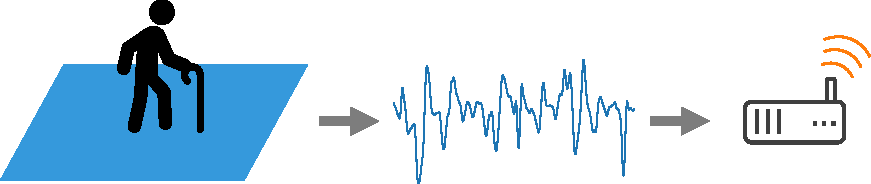
\includegraphics[width=0.95\linewidth]{schema_fall_detector.pdf}\\
        %         \onslide<1->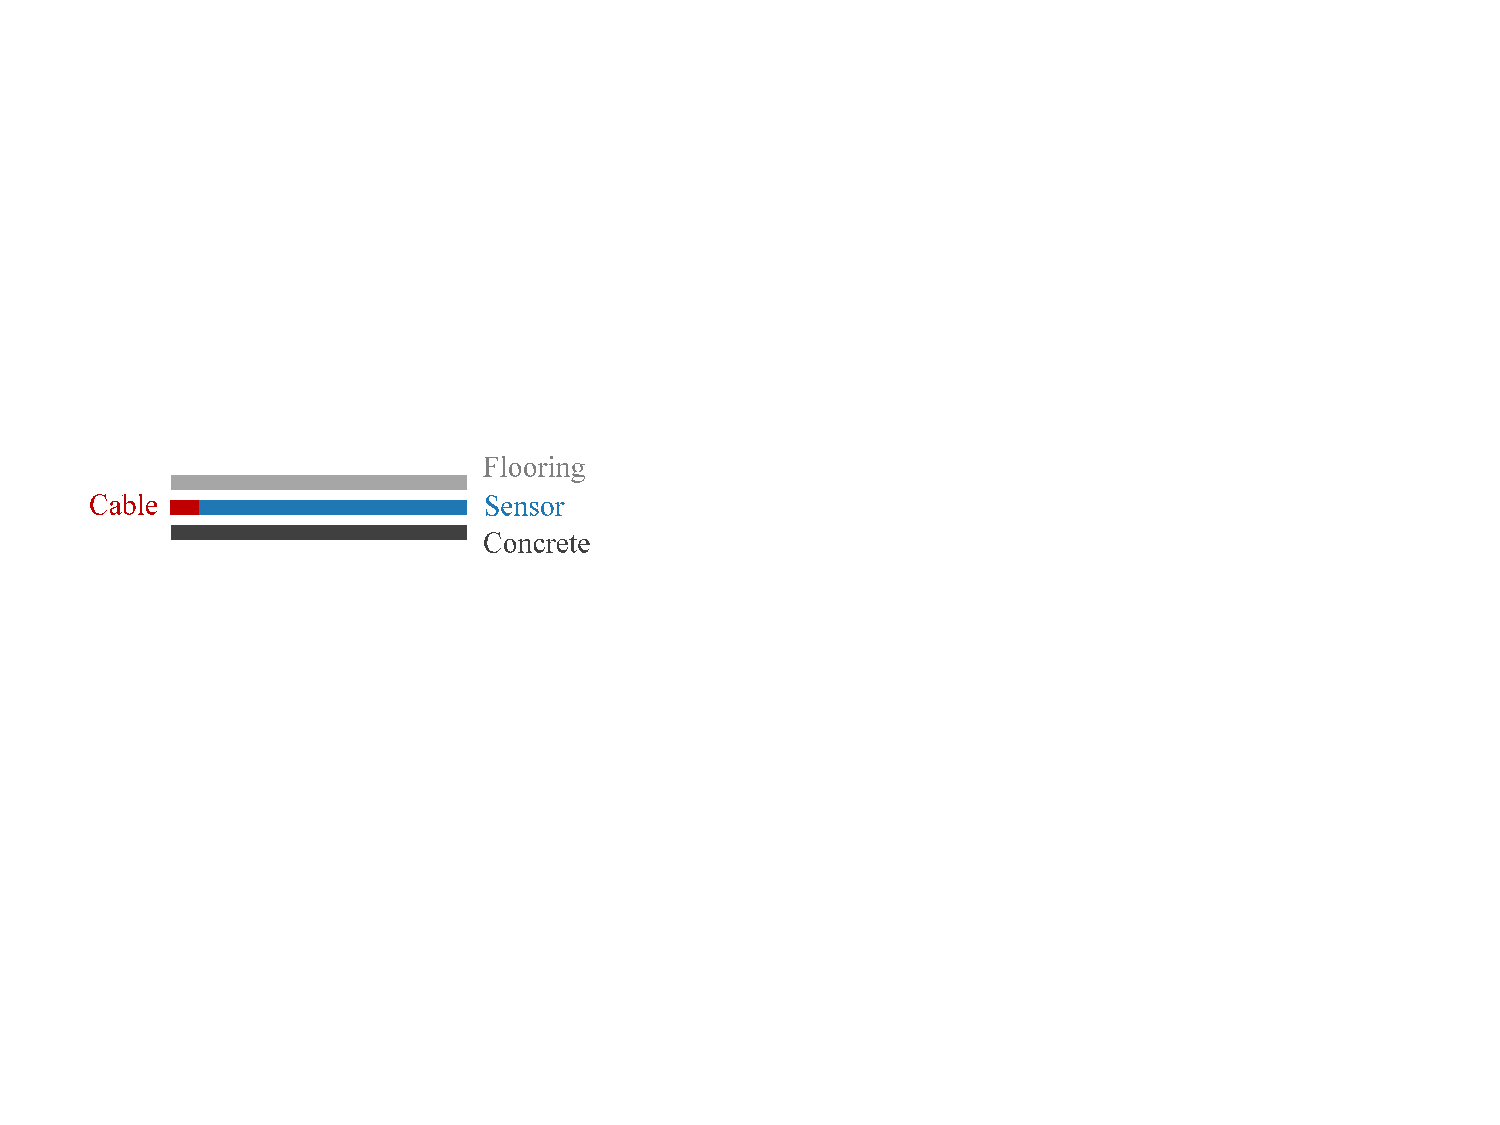
\includegraphics[width=0.4\linewidth, trim={20 230 430 200}, clip]{schema_sensor_installation_3.pdf}\\[5pt]
%                 \onslide<2->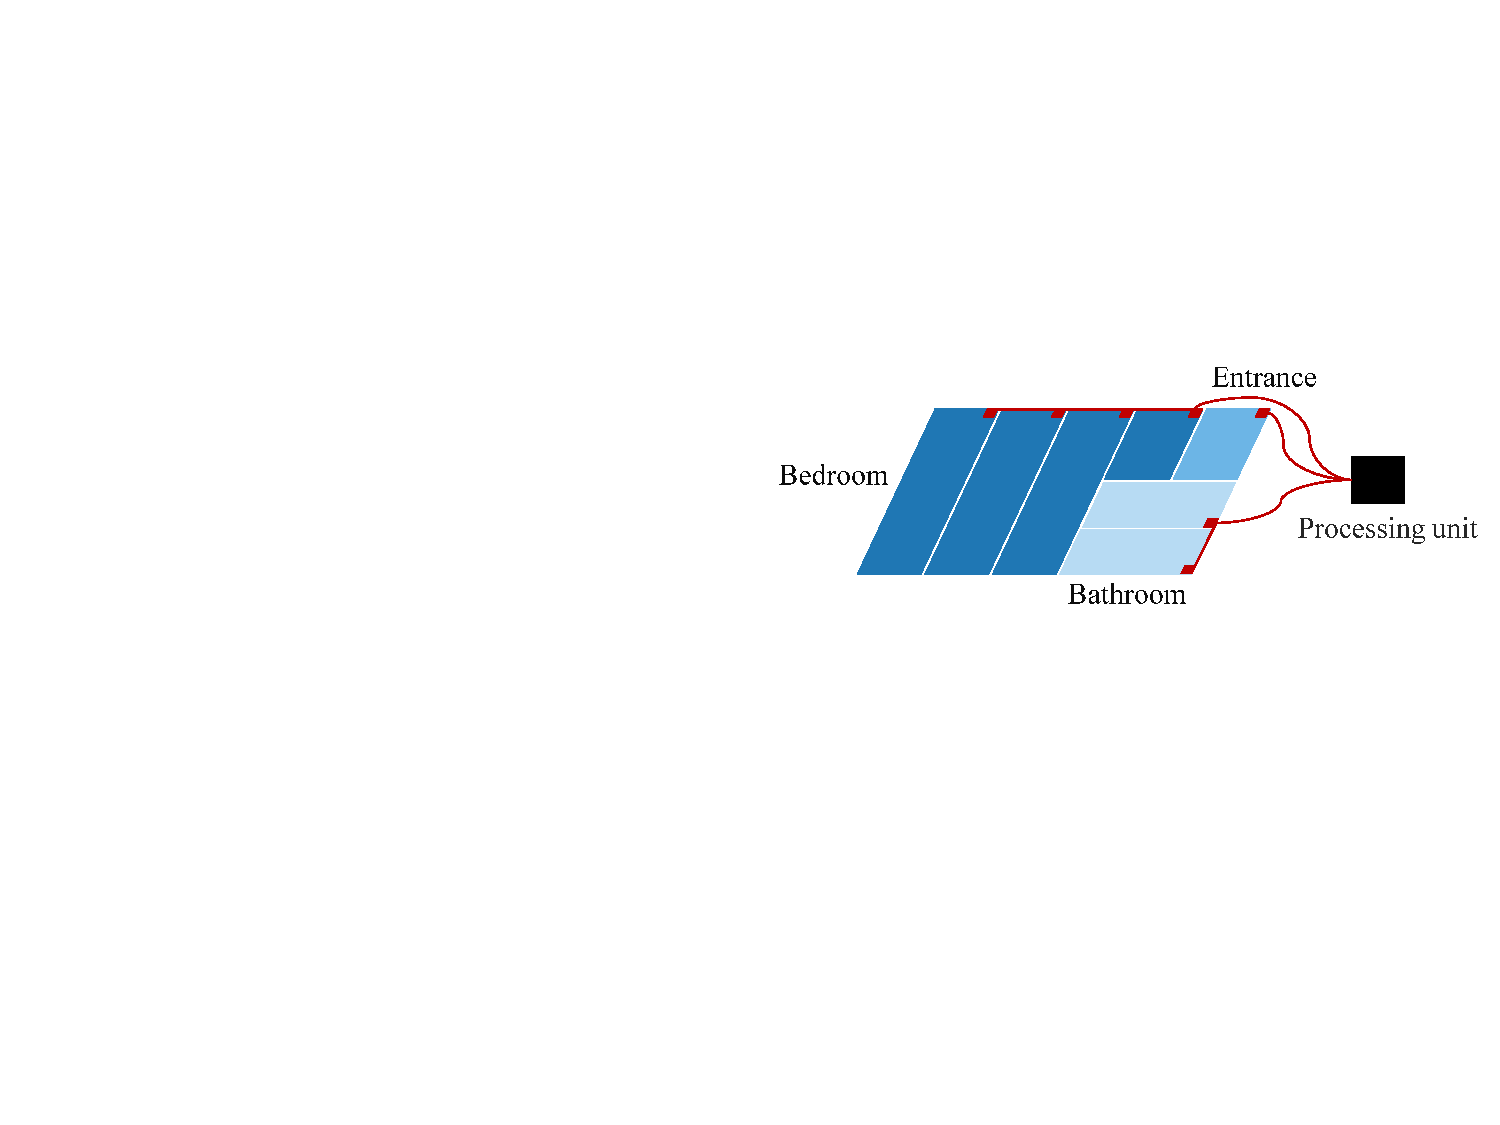
\includegraphics[width=0.4\linewidth, trim={360 230 5 160}, clip]{schema_sensor_installation_room_3.pdf}
        %         \onslide<2->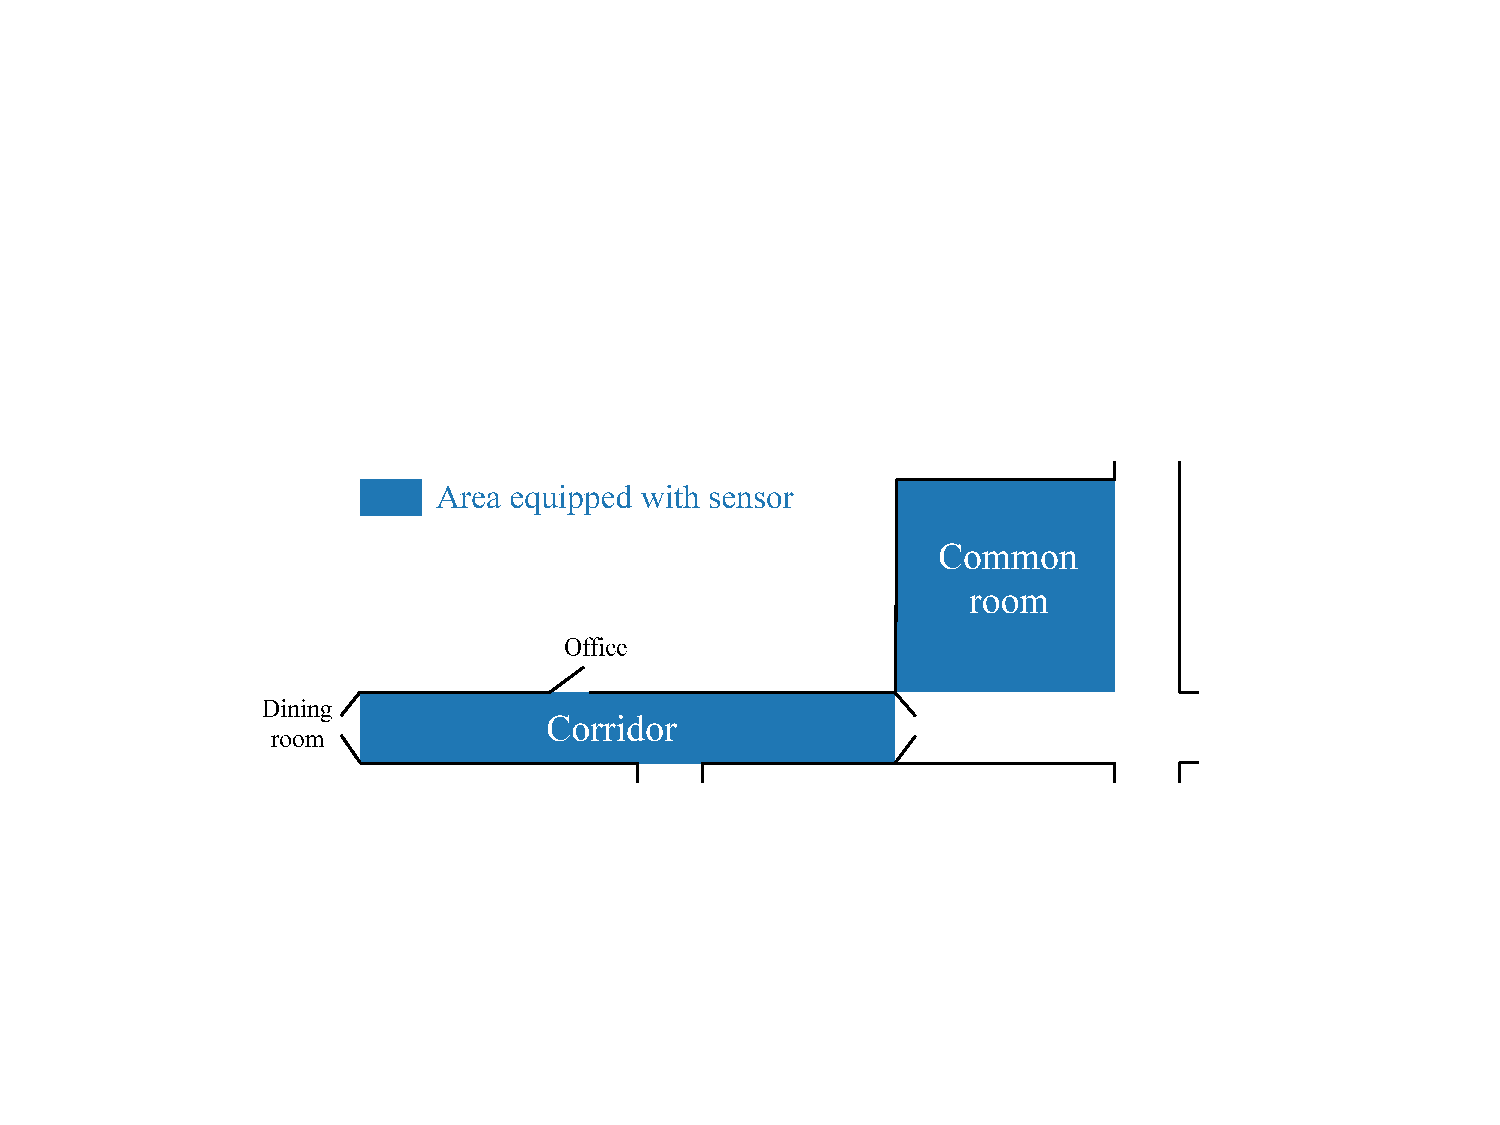
\includegraphics[width=0.6\linewidth, trim= 50 150 50 210, clip]{schema_couloir_plan_blue.pdf}
        %     \end{minipage}
        %     \caption{System installation in a nursing home.}
        %     \label{fig:schema_installation}
%         \end{figure}
    \end{minipage}
\end{minipage}
\end{frame}

\begin{frame}{Introduction}{}
% \hspace{4cm}
\begin{minipage}[t]{\linewidth}
%     \centering
    \textbf{Motivation}
    \begin{itemize}
        \item Processing and understanding time series
        \begin{itemize}
            \item Proliferation of sensor-based systems
            \item Redundancy, interpretability, external pertubations
        \end{itemize}
        \item Real world application
        \begin{itemize}
            \item Real-time processing in a limited system
            \item Convenient hypotheses not granted
        \end{itemize}
    \end{itemize}
\end{minipage}

\vspace{1cm}
\renewcommand{\ratio}{0.4}
% \begin{figure}[b]
    \centering
    \begin{minipage}{\linewidth}
        \centering
        \begin{minipage}{\ratio\linewidth}
            \centering
            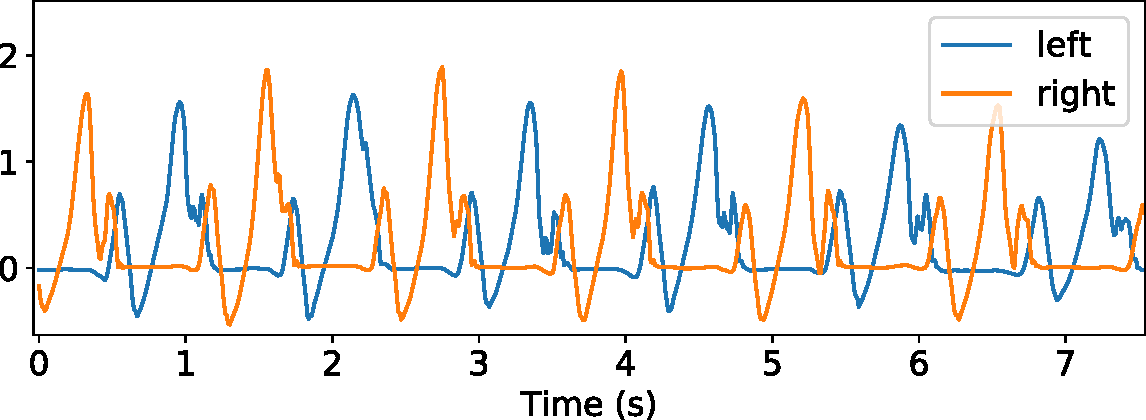
\includegraphics[width=0.91\linewidth]{signal_marche_accelerometre_left_right_epure.pdf}\\
            {\small Foot-attached accelerometer}
        \end{minipage}
        \begin{minipage}{\ratio\linewidth}
            \centering
            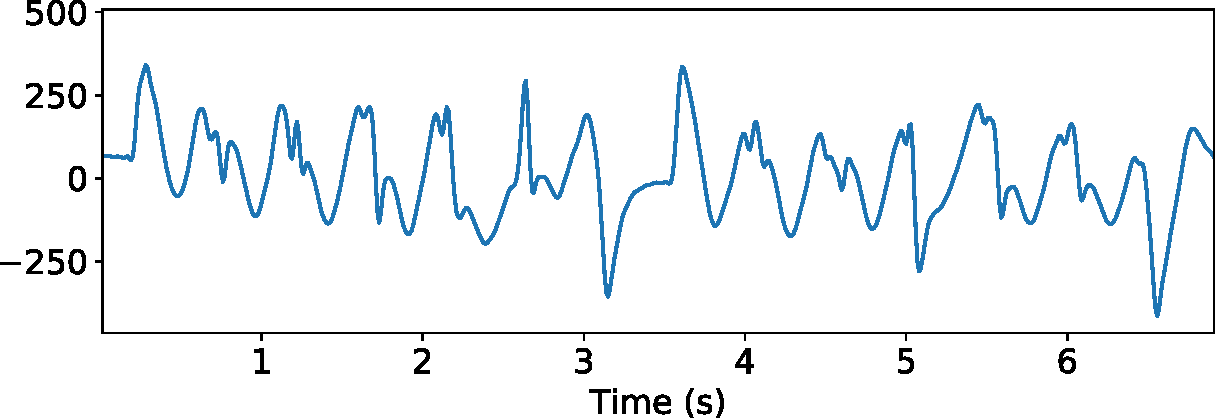
\includegraphics[width=\linewidth]{signal_marche_tarkett_epure.pdf}\\
            {\small Tarkett's floor sensor}
        \end{minipage}
    \end{minipage}
%     \caption{Example of walk signals from different sensors.}
%     \label{fig:introduction_signals_walk}
% \end{figure}

\end{frame}

\section{A tour of monitoring systems}
\subsection{Systems}
\begin{frame}{A tour of monitoring systems}{Systems}
    
    \begin{minipage}[t]{0.49\linewidth}
        \vspace{0pt}
What makes a good monitoring system ?
        \begin{itemize}
            \item coverage and occlusion
            \item intrusiveness
            \item signal quality / information
            \item robustness
            \item ease of installation / use
            \item scalability
        \end{itemize}

    \end{minipage}\hfill
    \begin{minipage}[t]{0.49\linewidth}
        \vspace{0pt}
        \begin{overprint}
            \onslide<2>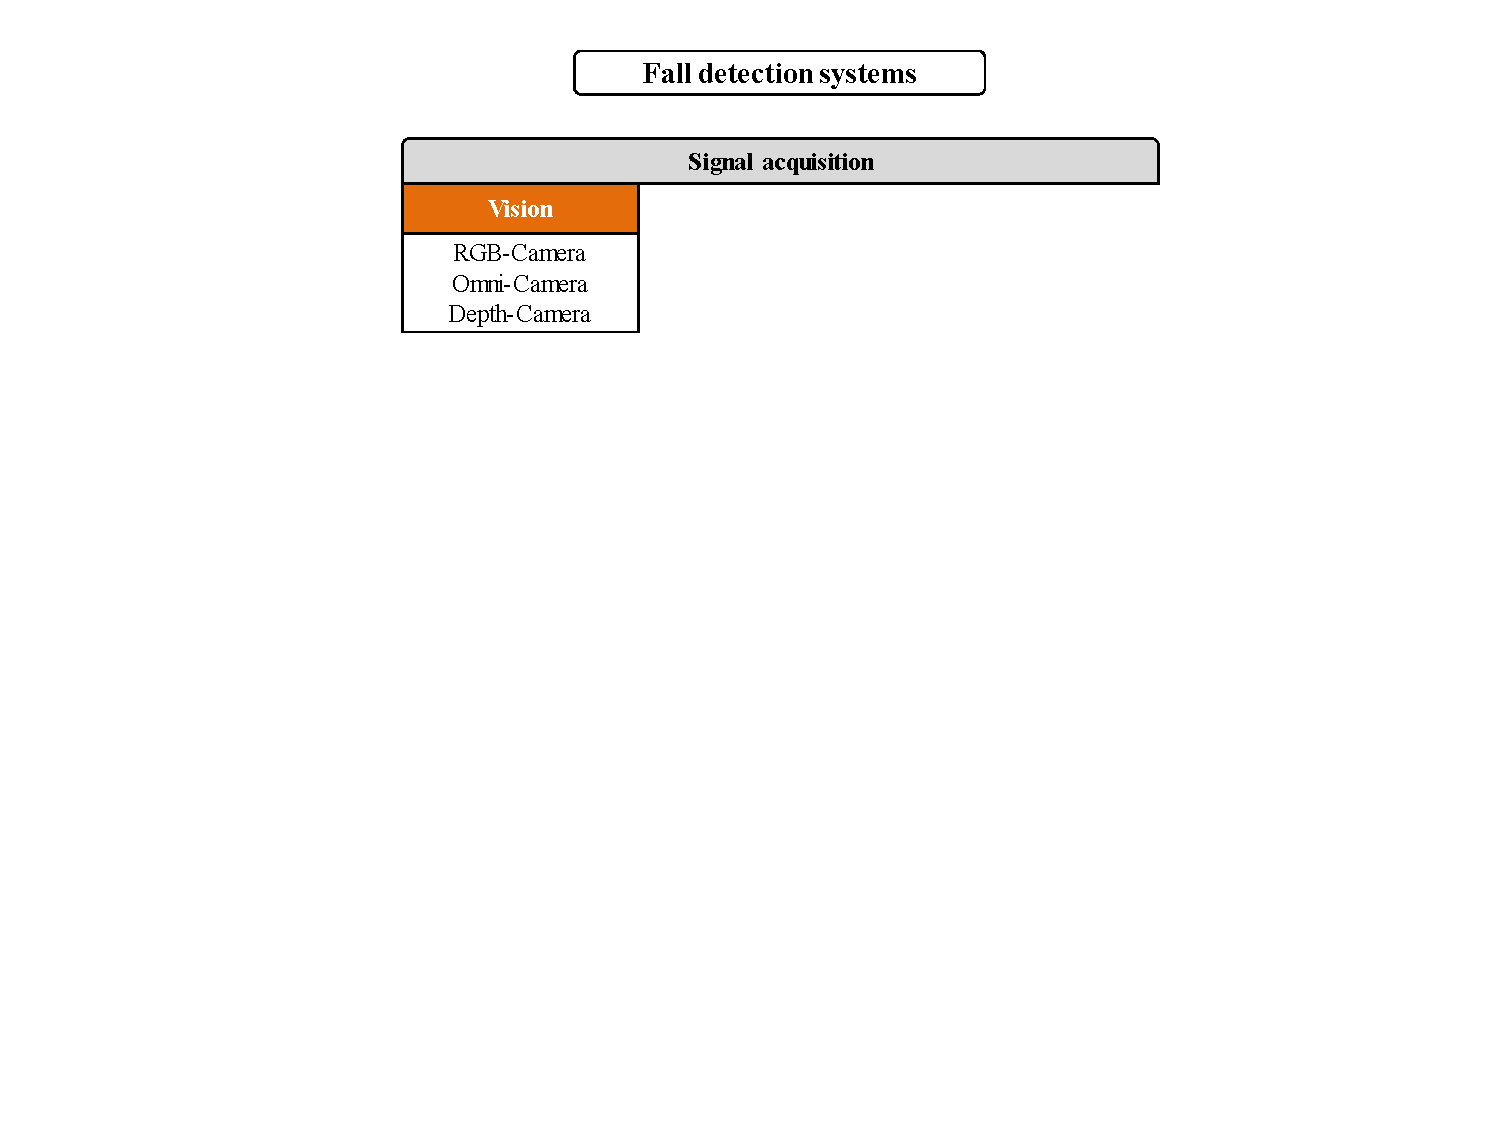
\includegraphics[width=\linewidth, trim={190 250 150 60}, clip]{fall_systems_1_1-14.pdf}
            \onslide<3>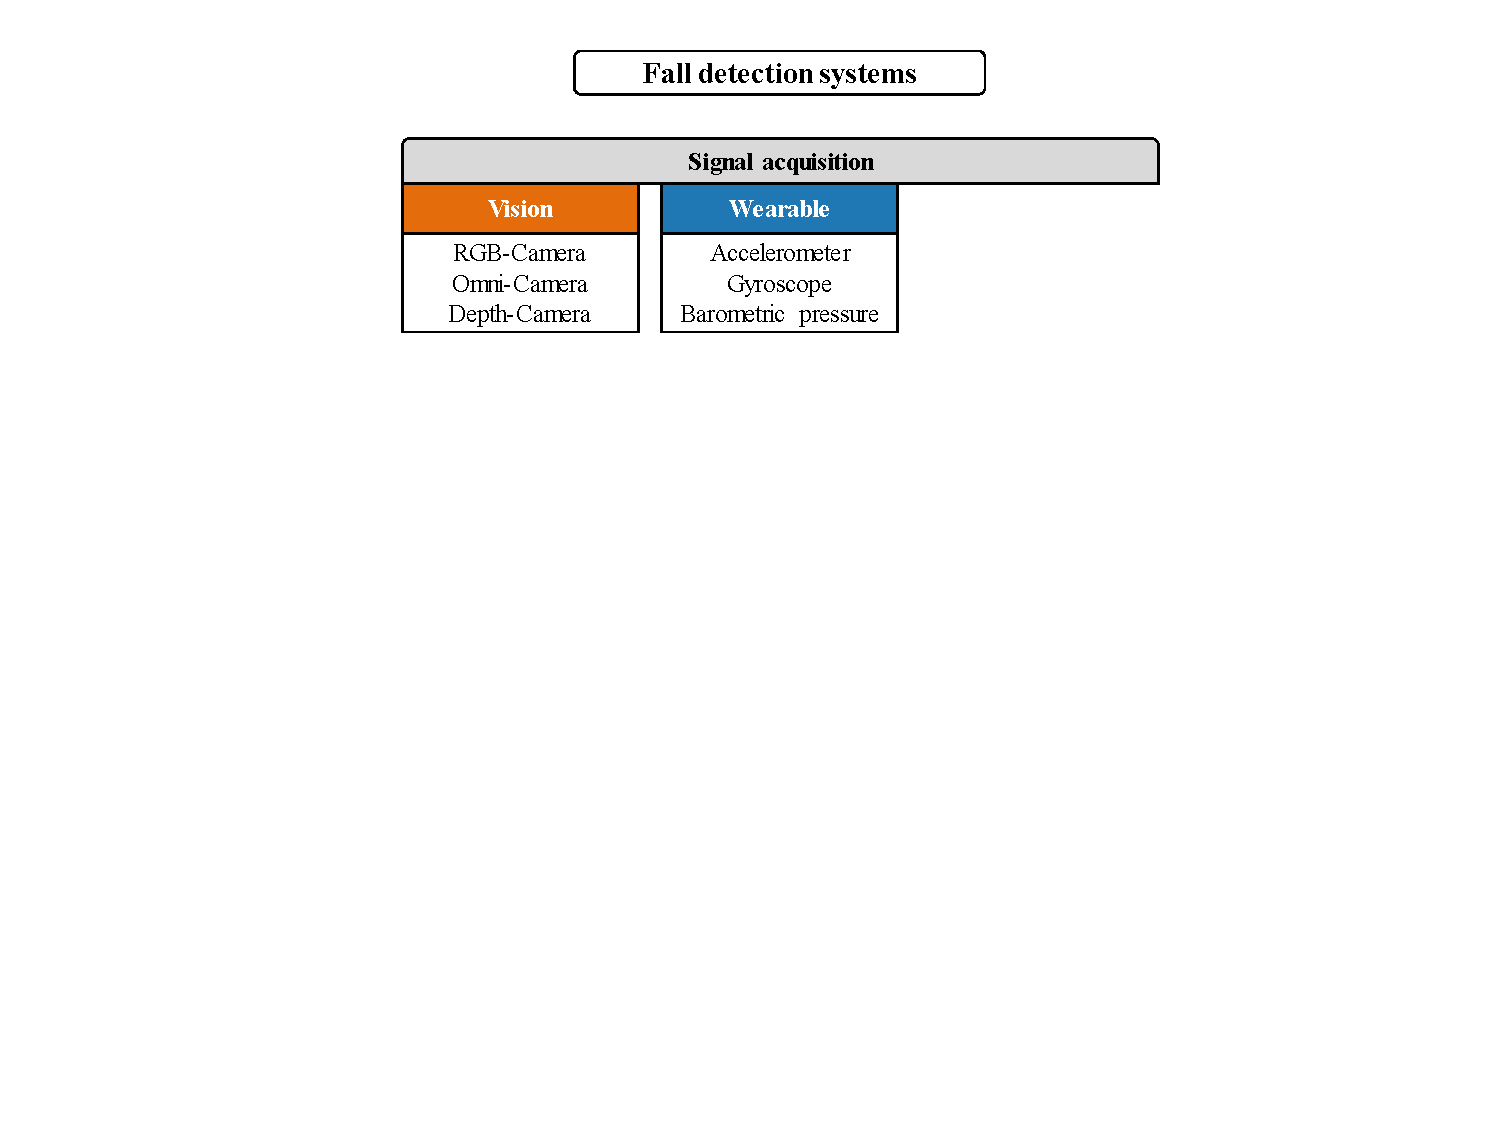
\includegraphics[width=\linewidth, trim={190 250 150 60}, clip]{fall_systems_1_2-14.pdf}
            \onslide<4>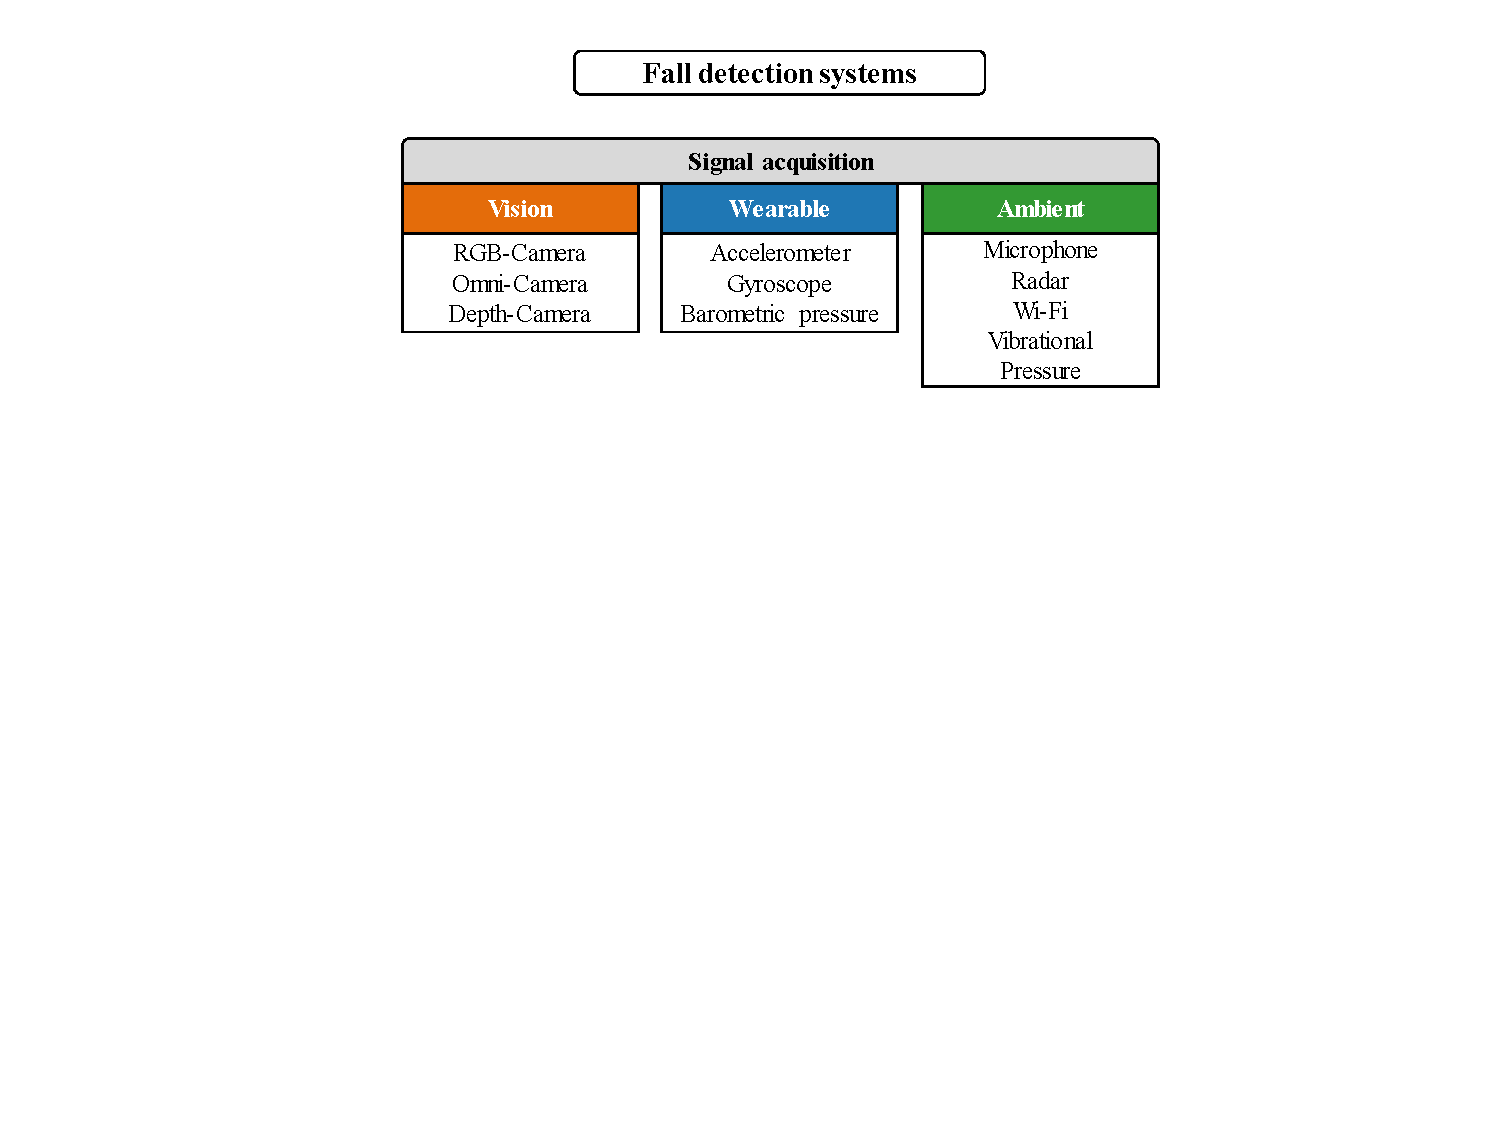
\includegraphics[width=\linewidth, trim={190 250 150 60}, clip]{fall_systems_1_3-14.pdf}
        \end{overprint}
    \end{minipage}
% \end{minipage}

\vspace{-0.8cm}
% \onslide<1>{
\renewcommand{\arraystretch}{1.1}
\newcommand{\myvar}{45}
\begin{table}[]
\centering
\footnotesize
% \small
    \begin{tabular}{l c c c c c c c}
%     \hline
    Criteria & \onslide<2->{\rotatebox{\myvar}{RGB cam} & \rotatebox{\myvar}{Depth cam}} & \onslide<3->{\rotatebox{\myvar}{Wearable}} & \onslide<4->{\rotatebox{\myvar}{Acoustic} & \rotatebox{\myvar}{Radar / Wi-Fi} & \rotatebox{\myvar}{Vibration} & \rotatebox{\myvar}{Floor}} \\
    \midrule
    Coverage/Occlusion & \onslide<2->{\starb\starw\starw & \starb\starw\starw} & \onslide<3->{\starb\starb\starb} & \onslide<4->{\starb\starb\starw & \starb\starw\starw & \starb\starb\starb & \starb\starb\starb} \\
    Intrusiveness & \onslide<2->{\starb\starw\starw & \starb\starw\starw} & \onslide<3->{\starb\starb\starw} & \onslide<4->{\starb\starw\starw & \starb\starb\starw & \starb\starb\starb & \starb\starb\starb} \\
    Signal quality / info &\onslide<2->{\starb\starb\starb & \starb\starb\starb} & \onslide<3->{\starb\starb\starw} & \onslide<4->{\starb\starb\starw & \starb\starw\starw & \starb\starb\starw & \starb\starb\starw} \\
    Robustness & \onslide<2->{\starb\starb\starw & \starb\starb\starb} & \onslide<3->{\starb\starb\starb} & \onslide<4->{\starb\starw\starw & \starb\starw\starw & \starb\starw\starw & \starb\starb\starw} \\
    Ease of instal. / use & \onslide<2->{\starb\starw\starw & \starb\starw\starw} & \onslide<3->{\starb\starb\starw} & \onslide<4->{\starb\starb\starw & \starb\starb\starw & \starb\starb\starb & \starb\starw\starw} \\
    Scalability & \onslide<2->{\starb\starw\starw & \starb\starw\starw} & \onslide<3->{\starb\starb\starb} & \onslide<4->{\starb\starb\starw & \starb\starw\starw & \starb\starb\starw & \starb\starb\starb} \\
    \midrule
    \end{tabular}
% \caption{Sensors evaluation over key criteria for patient monitoring systems.}
\label{tab:fall_detection_sensors_comparison}
\end{table}
\renewcommand{\arraystretch}{1.0}
% }

\end{frame}

\subsection{Information extraction}
\begin{frame}{A tour of monitoring systems}{Information extraction}

% \begin{minipage}[t]{\linewidth}
    \begin{minipage}[t]{0.49\linewidth}
    \vspace{0pt}
    How to process the inputs ?
    \begin{itemize}
        \item All systems use feature extraction
        \item The ``level'' of feature engineering depends on the complexity / dimensionality of the input signal
    \end{itemize}
    How to deal with processed signals ?
    \begin{tcolorbox}[title=Time series classification]
%         \textbf{Time series classification}\\[-5pt]
        \begin{enumerate}
            \item Series as \emph{sequences}
            \begin{itemize}
                \item Distance-based methods
            \end{itemize}
            \item Series as \emph{feature vectors}
            \begin{itemize}
                \item Computing several measures over a fixed size
                \item Classification models
                (Anomaly detection, classical supervised models...)
            \end{itemize}
        \end{enumerate}
    \end{tcolorbox}
%     \vfill
%     \vspace{10cm}
    \end{minipage}
    \hfill
    \begin{minipage}[t]{0.49\linewidth}
    \vspace{0pt}
        \begin{overprint}
%             \onslide<3>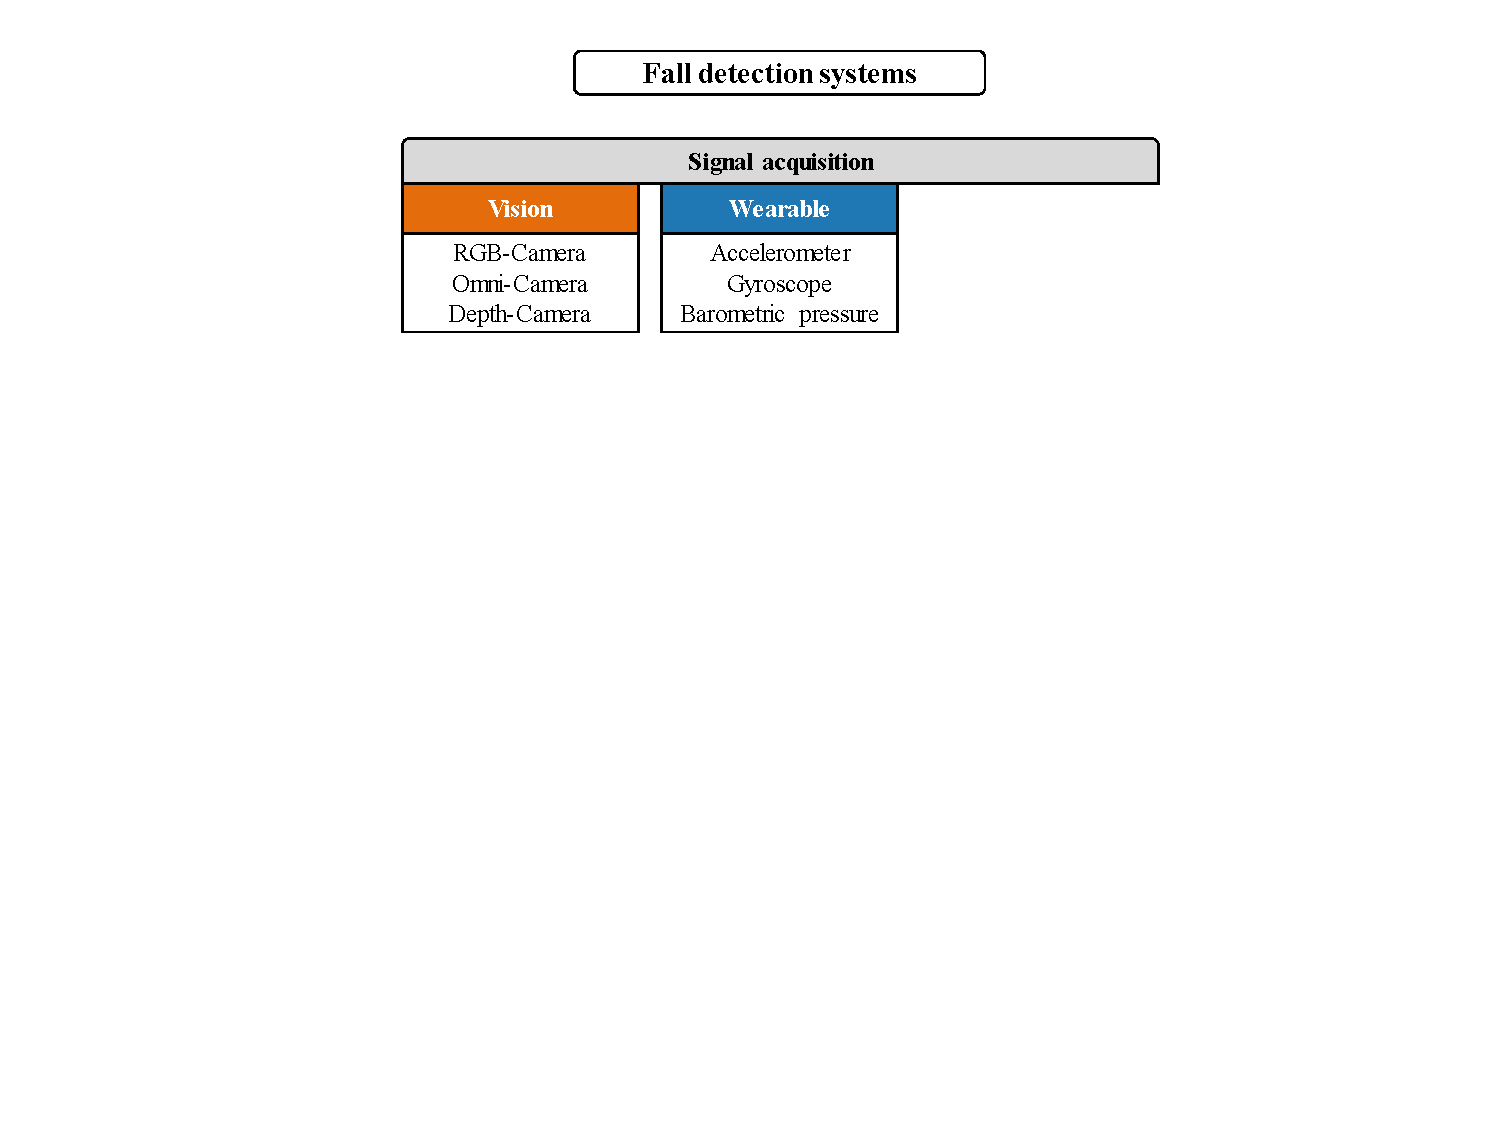
\includegraphics[width=\linewidth, trim={190 50 150 20}, clip]{fall_systems_1_2-14.pdf}
%             \onslide<4>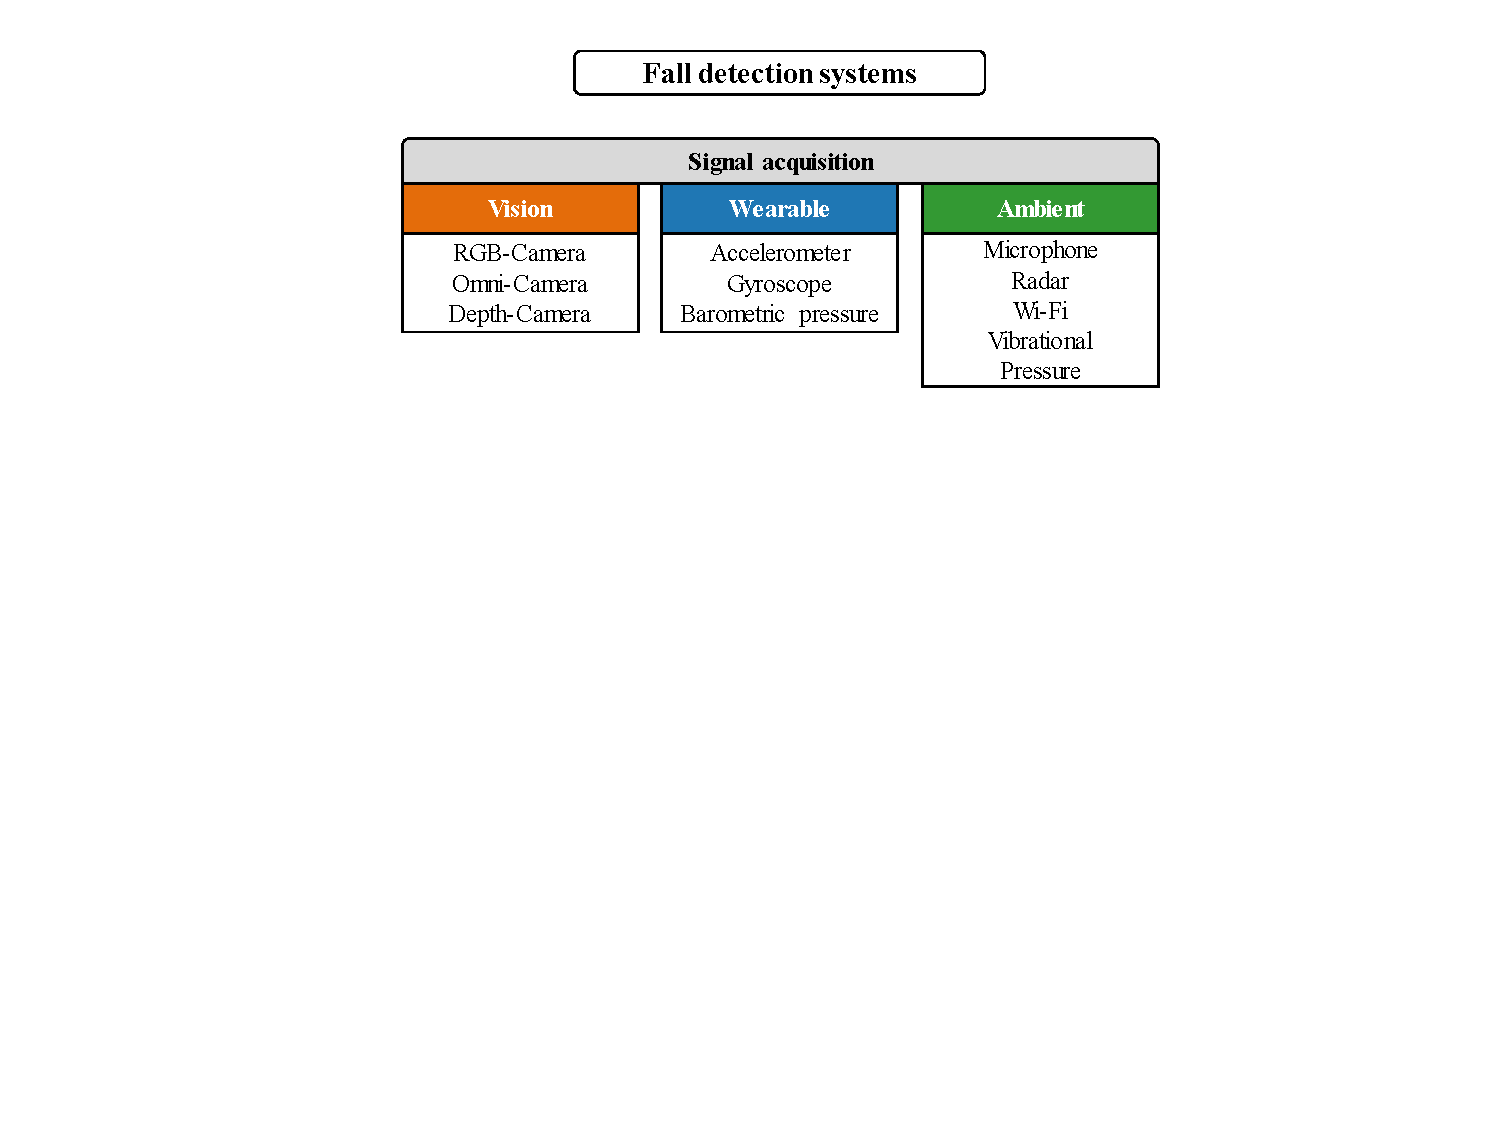
\includegraphics[width=\linewidth, trim={190 50 150 20}, clip]{fall_systems_1_3-14.pdf}
            \onslide<1>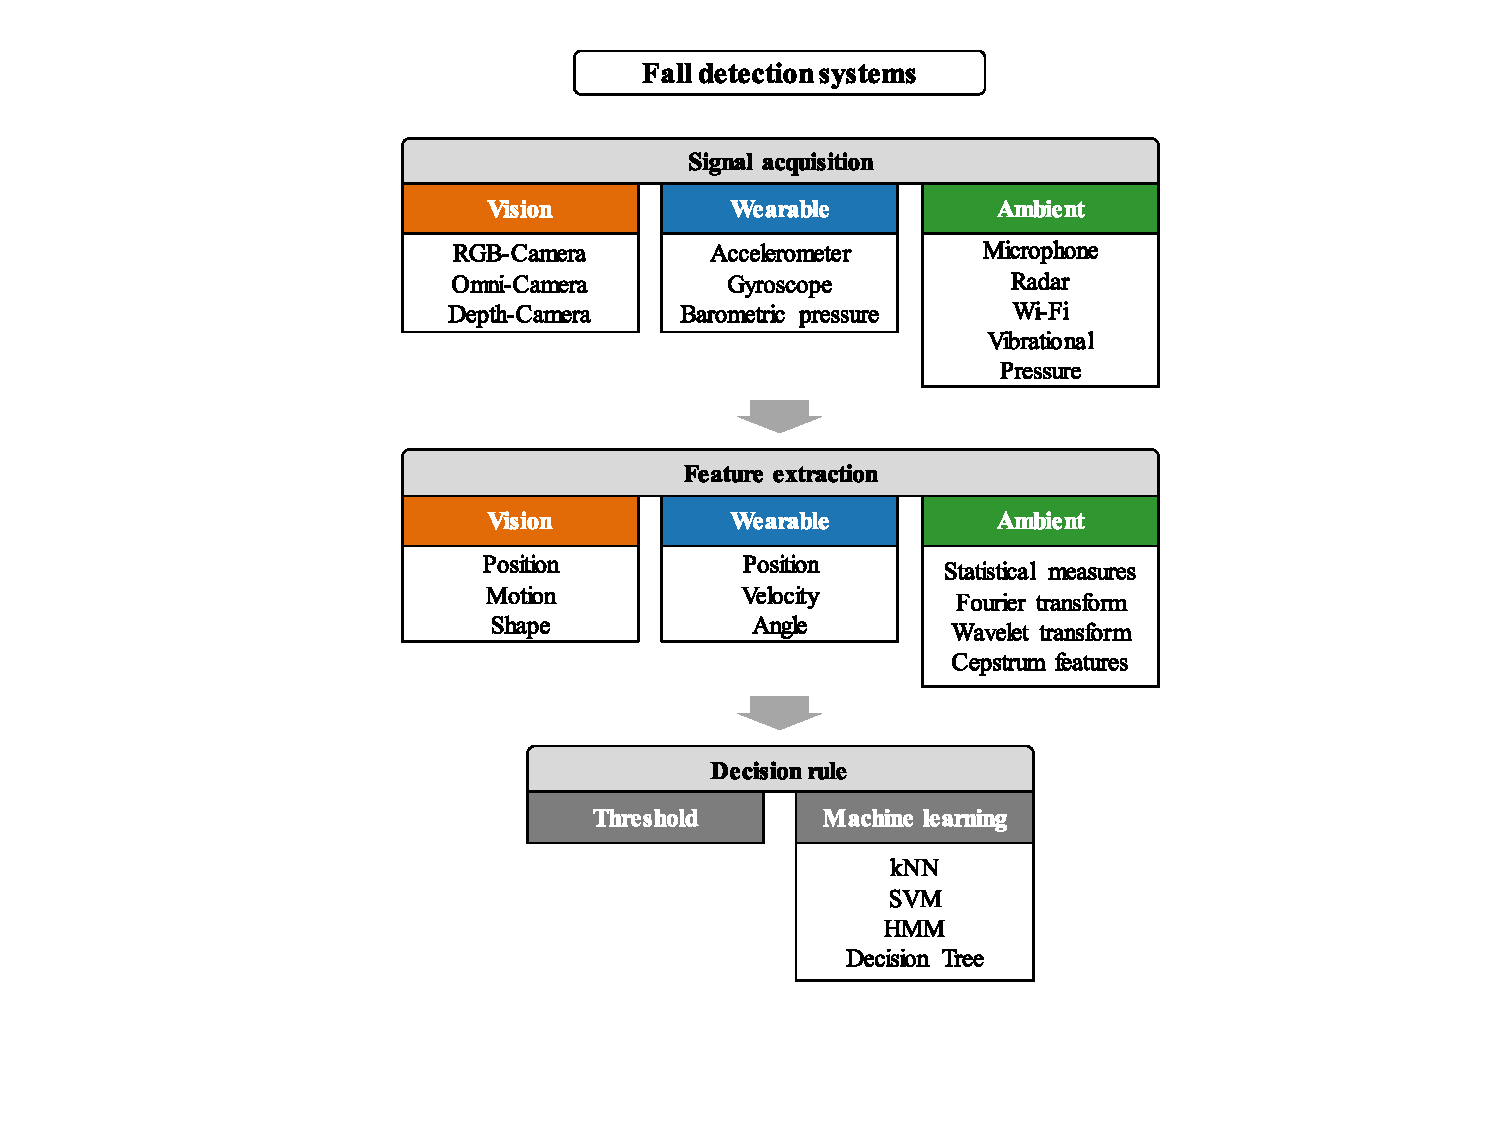
\includegraphics[width=\linewidth, trim={190 50 150 60}, clip]{fall_systems_3-14.pdf}
        \end{overprint}
    \end{minipage}
% \end{minipage}
\end{frame}

\subsection{Tarkett sensor}
\begin{frame}{A tour of monitoring systems}{Tarkett sensor}
% \begin{figure}[ht]
\begin{minipage}[t]{0.35\linewidth}
    \vspace{0pt}
    \begin{itemize}
        \item Piezoelectric principle: $$d = \frac{Q}{F}\;,$$ (simple version) with d the \emph{piezoelectric constant}.\\
        When stressed or squeezed, the material emits charges.\\
        \pause
        \item How does this look like ?\\
            0.3 mm thick and 60 cm wide roll with customizable length
        \pause
        \item How is it installed ?\\
            \begin{itemize}
                \item Under the flooring
                \item Several connected bands for each area, hence one area corresponds to one input
            \end{itemize}

    \end{itemize}
\end{minipage}\hfill
\begin{minipage}[t]{0.64\linewidth}
    \vspace{0pt}
% \begin{minipage}{\linewidth}
    \centering
    % left bottom right top
    \onslide<1->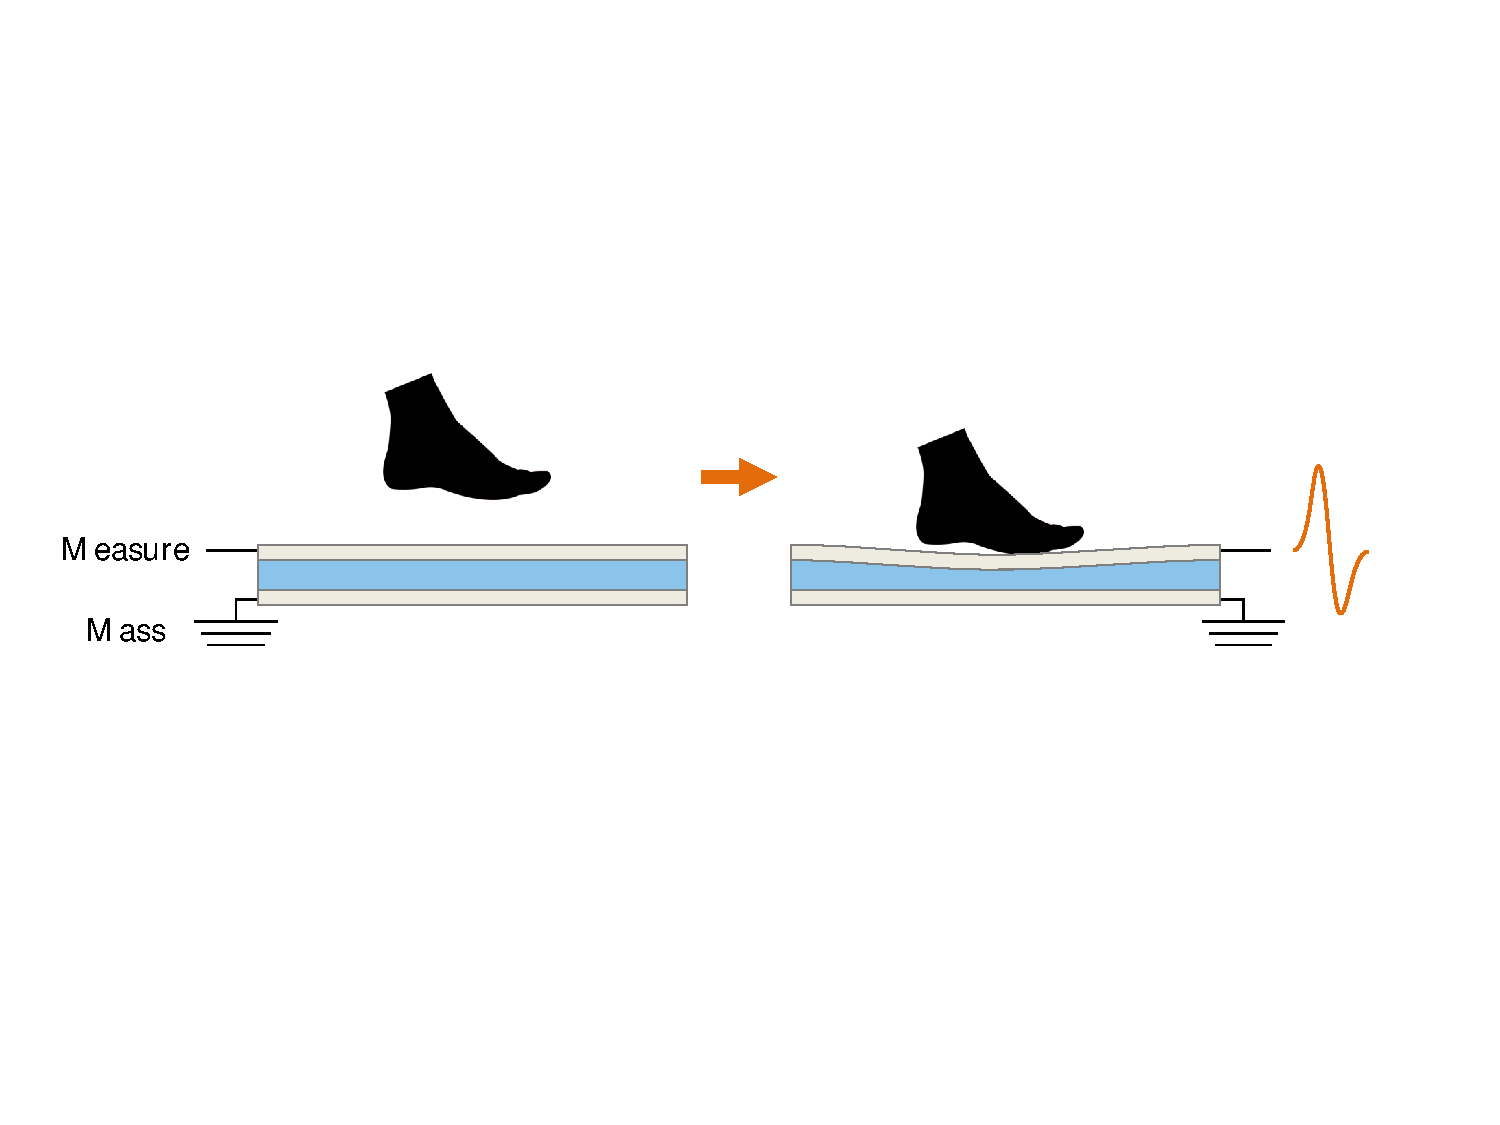
\includegraphics[width=0.9\linewidth, trim={20 220 60 170}, clip]{schema_piezo.pdf}\\
% \caption{Piezoelectric sensor principle.
%          When deformed, the piezoelectric material emits charges, hence a current can be measured in output.
%          }
% \label{fig:schema_piezoelectric}
% \end{figure}
%     \renewcommand{\ratio}{0.4}
    \begin{minipage}[t]{0.49\linewidth}
        \centering
        \onslide<2->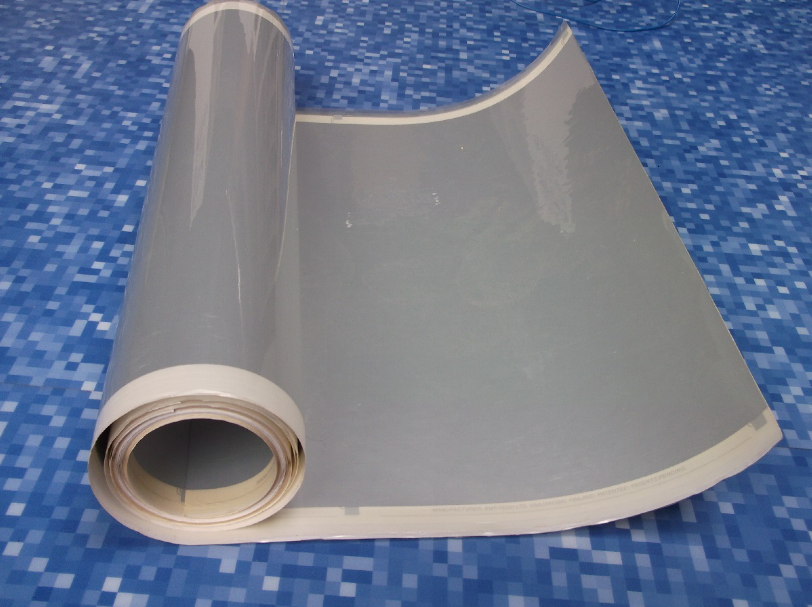
\includegraphics[width=\linewidth, height=1.9cm, keepaspectratio, trim={0 0 0 0}, clip]{photo_capteur_rouleau.png}\\
%         \small Roll of sensor
    \end{minipage}
    \begin{minipage}[t]{0.49\linewidth}
        \centering
        \onslide<2->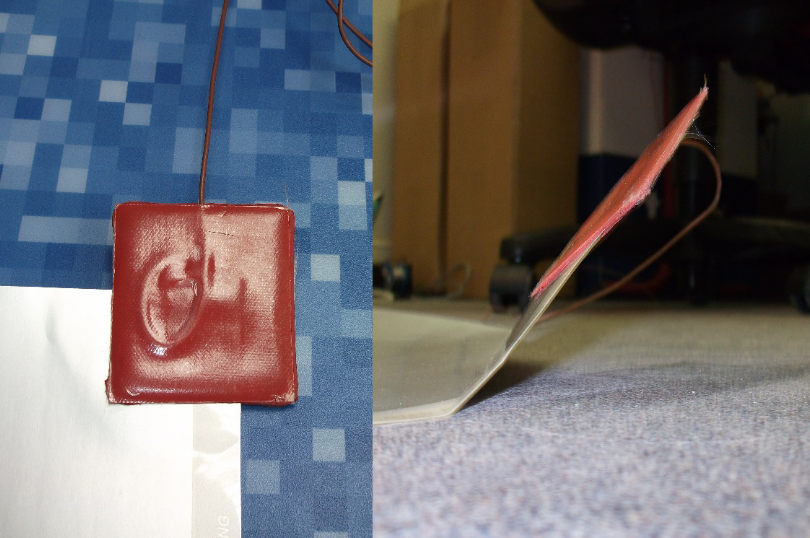
\includegraphics[width=\linewidth, height=1.9cm, keepaspectratio, trim={0 0 0 0}, clip]{photo_capteur_connecteur.png}\\
%         \small Connector
    \end{minipage}
    
% \begin{minipage}[t]{\linewidth}
    \begin{minipage}[b]{0.45\linewidth}
    \centering
    % left bottom right top
    \onslide<3->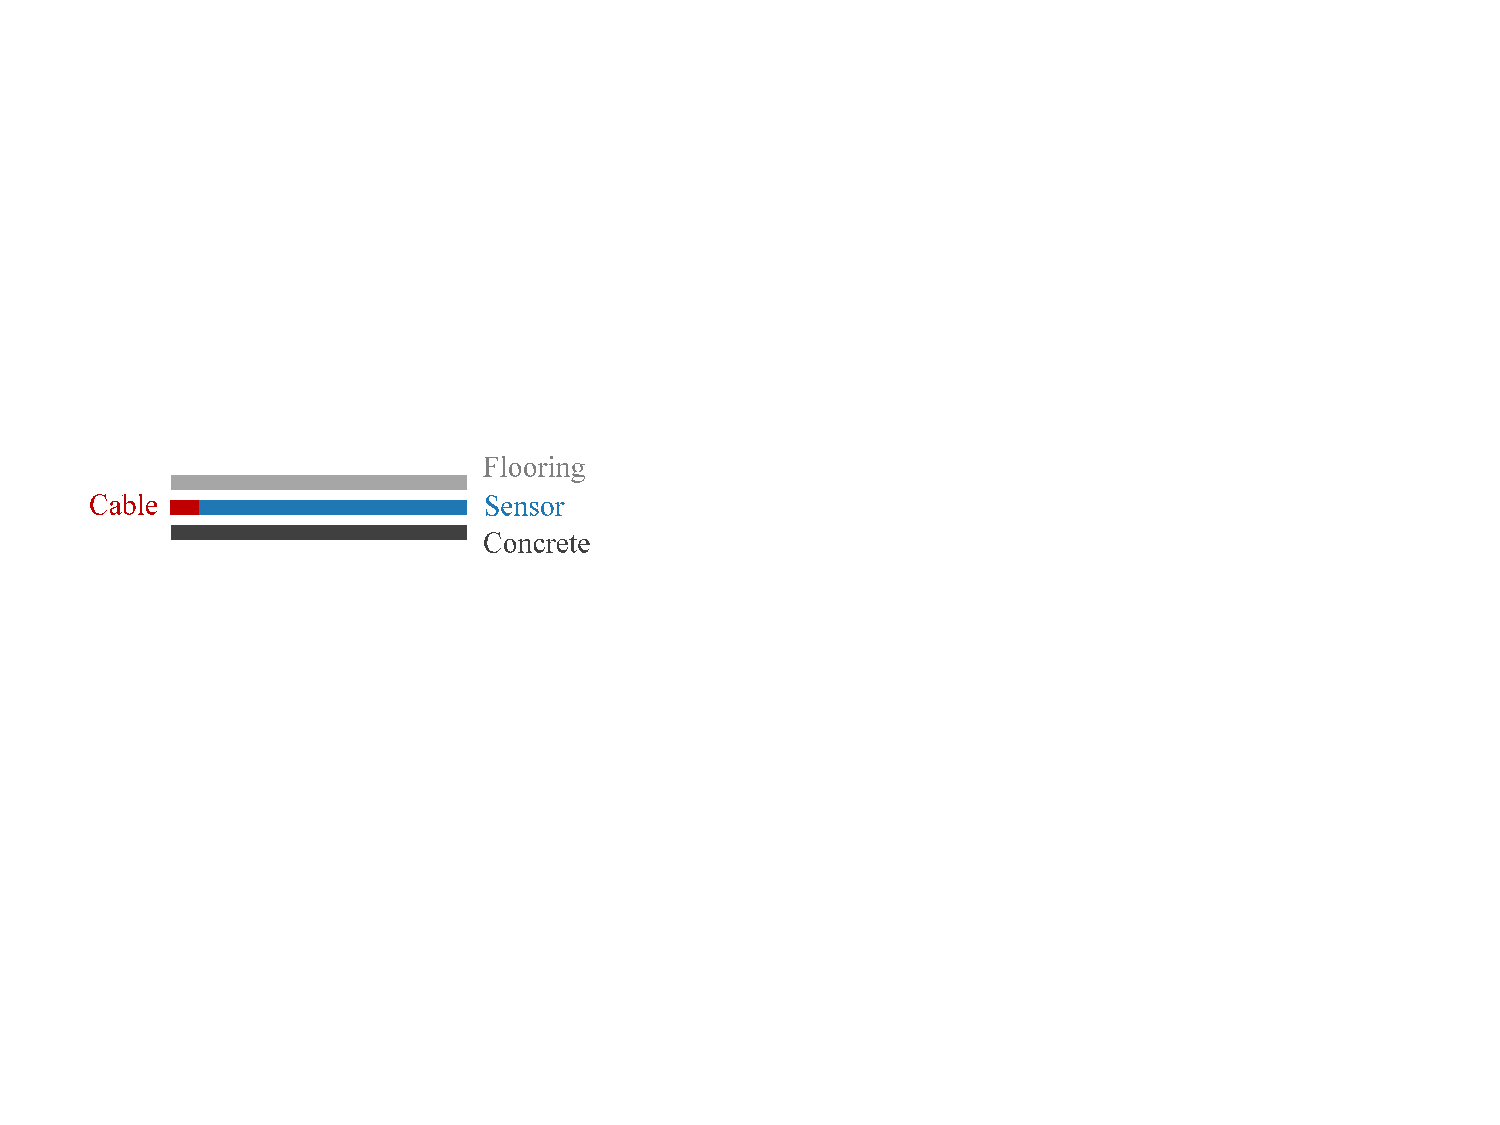
\includegraphics[width=0.95\linewidth, trim={20 260 430 200}, clip]{schema_sensor_installation_3.pdf}
    
%     \small Sensor set up
    \end{minipage}
    \hfill
    \begin{minipage}[b]{0.54\linewidth}
    \centering
    \onslide<3->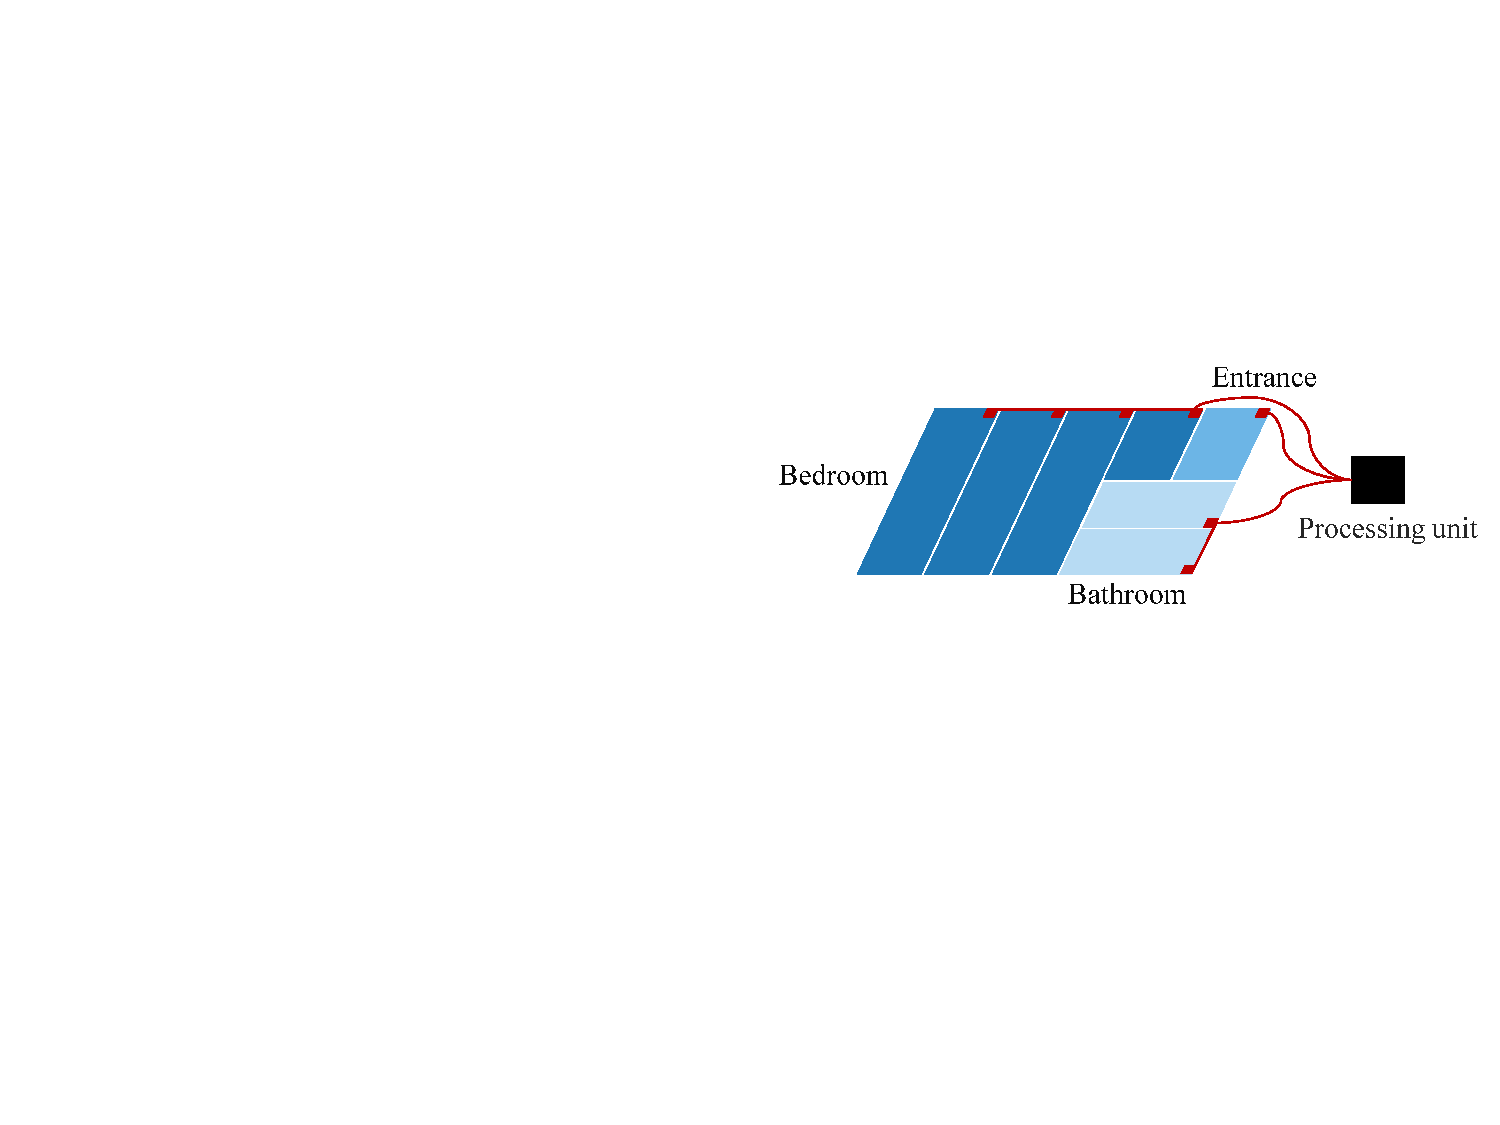
\includegraphics[width=\linewidth, trim={360 240 5 160}, clip]{schema_sensor_installation_room_3.pdf}
    
%     \small Room equipped with the system
    \end{minipage}
% \end{minipage}
\end{minipage}

\end{frame}

\section{A fall detection system}
\subsection{Data}
\begin{frame}{Fall detection}{Data}
\begin{minipage}[t]{0.49\linewidth}
    \vspace{0pt}
%     \begin{itemize}
        \textbf{Preprocessing}
        \begin{itemize}
            \item linear detrending
            \item low-pass filtering
            \item zeroing low energy channels
            \item sum over all channels
        \end{itemize}
%     \end{itemize}
    \medskip
    \begin{overprint}
%         \begin{minipage}{0.49\linewidth}
%         \centering
            \onslide<1>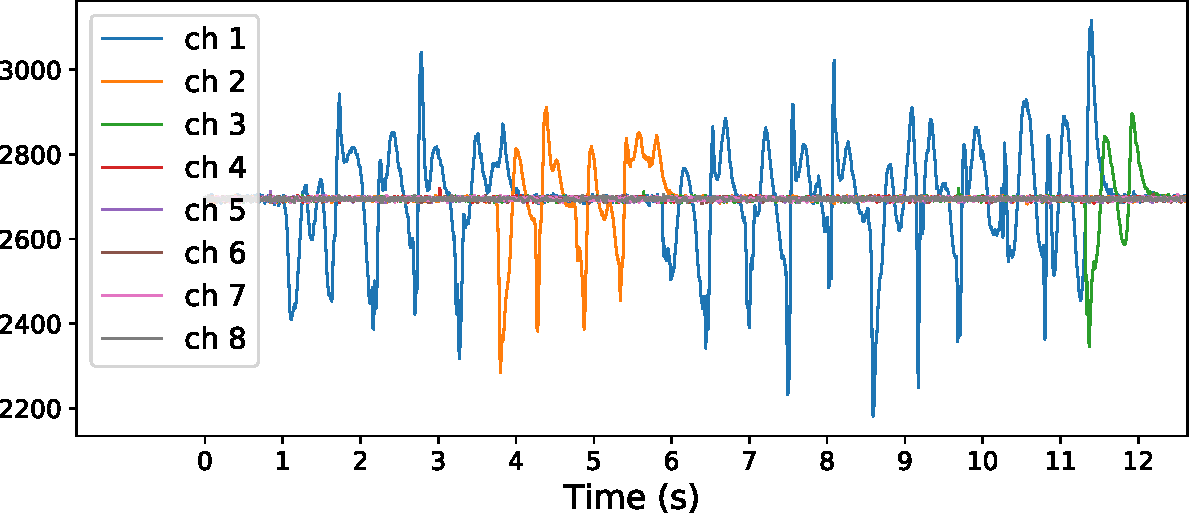
\includegraphics[trim= 0 0 0 0, width=0.8\linewidth, clip]{ex_signal_raw_2.pdf}
%             {\small Raw signal}
%         \medskip
%         \end{minipage}
%         \begin{minipage}{0.49\linewidth}
%         \centering
            \onslide<2->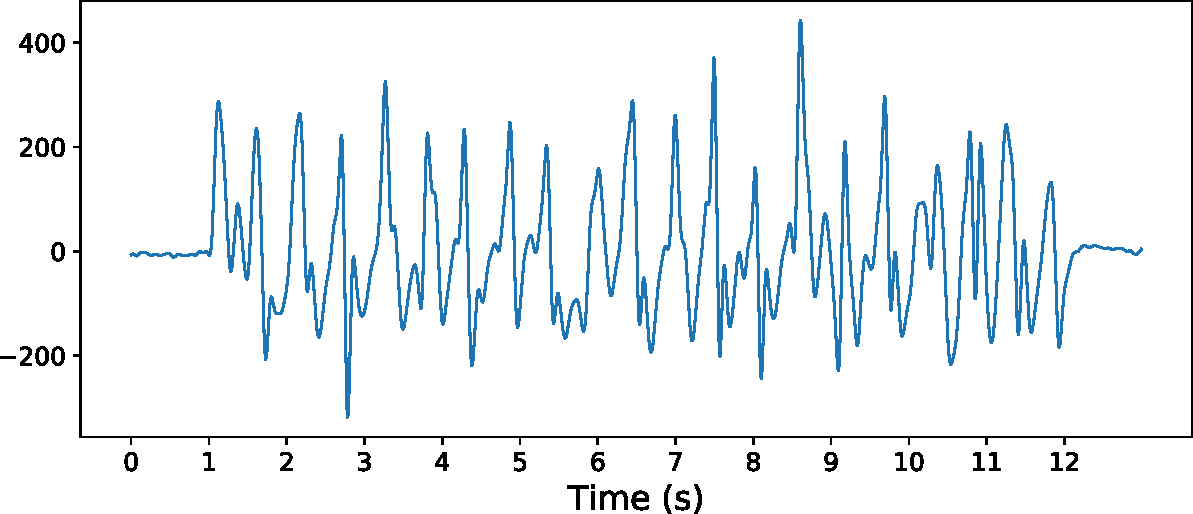
\includegraphics[trim= 0 0 0 0, width=0.8\linewidth, clip]{ex_signal_preproc_2.pdf}
%             {\small Preprocessed signal}
%         \medskip
%         \end{minipage}
    \end{overprint}
\end{minipage}\hfill
\begin{minipage}[t]{0.49\linewidth}
\vspace{0pt}
% \centering
%     \begin{itemize}
    \pause \pause
    \textbf{Experimental dataset}
    \begin{itemize}
        \item 742 signals
        \item 55\% \emph{fall}, 45\% \emph{non-fall}
        \item varied fall events (forward, backward...) and activities of daily living (walking, sitting...)
    \end{itemize}
%     \end{itemize}
    \medskip
    \centering
    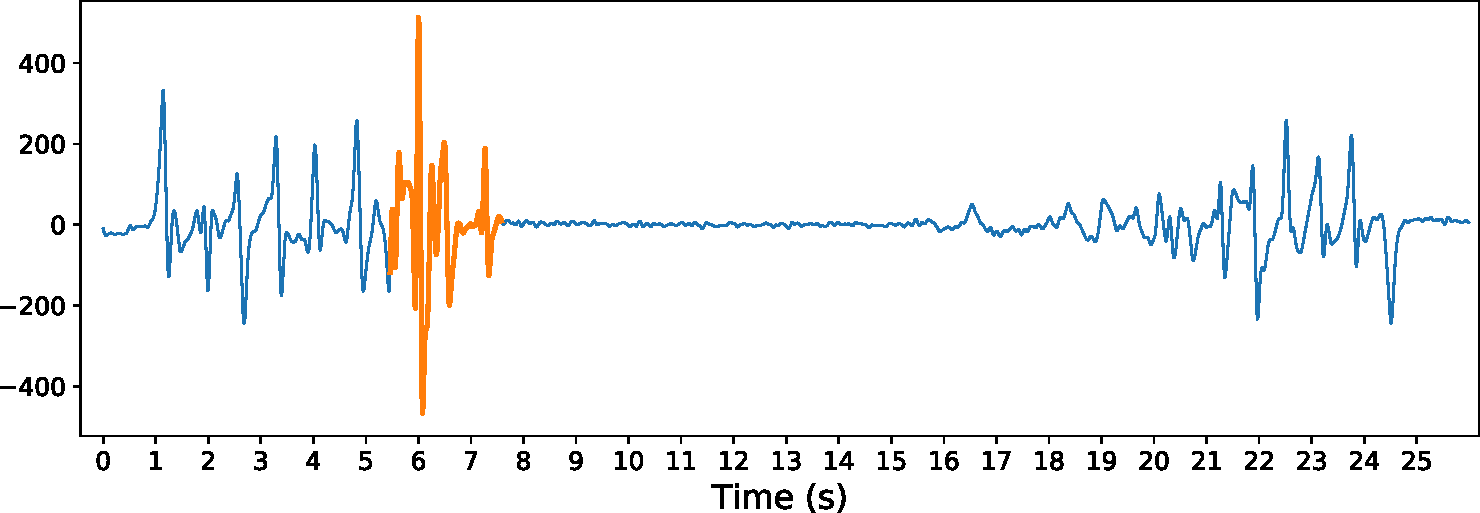
\includegraphics[width=0.85\textwidth]{ex_signal_chute_2.pdf}\\
    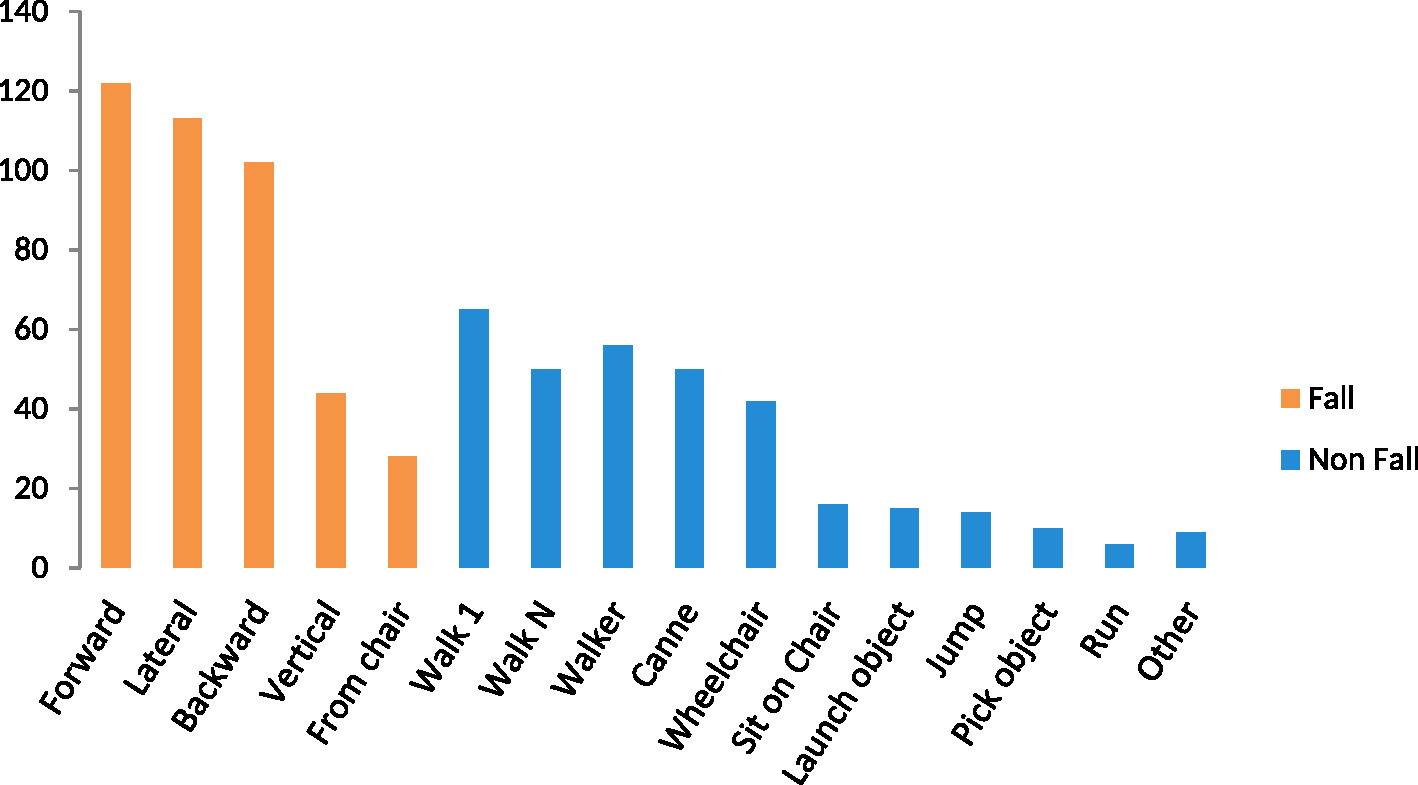
\includegraphics[width=0.8\linewidth]{exp_database_epure_2.pdf}

\end{minipage}

\end{frame}

\subsection{Method}
\begin{frame}{Fall detection}{Method}


\begin{minipage}[t]{0.49\linewidth}
    \vspace{0pt}
Time series as \emph{feature vector}. At every timestamp:
    \begin{enumerate}
        \item Window over the signal: 2.5 s
        \item Compute feature vector: 29 statistical measures (Min, Max, Shannon energy, Percentile,...) over three representations of the signal
    \end{enumerate}
    \centering
    \begin{overlayarea}{\linewidth}{0cm}
    \centering
    \only<1>{%
    \begin{tikzpicture}[line cap=round,line join=round,>=triangle 45,x=0.2cm,y=0.4cm]
    \node[inner sep=0pt] at (0,0)
        {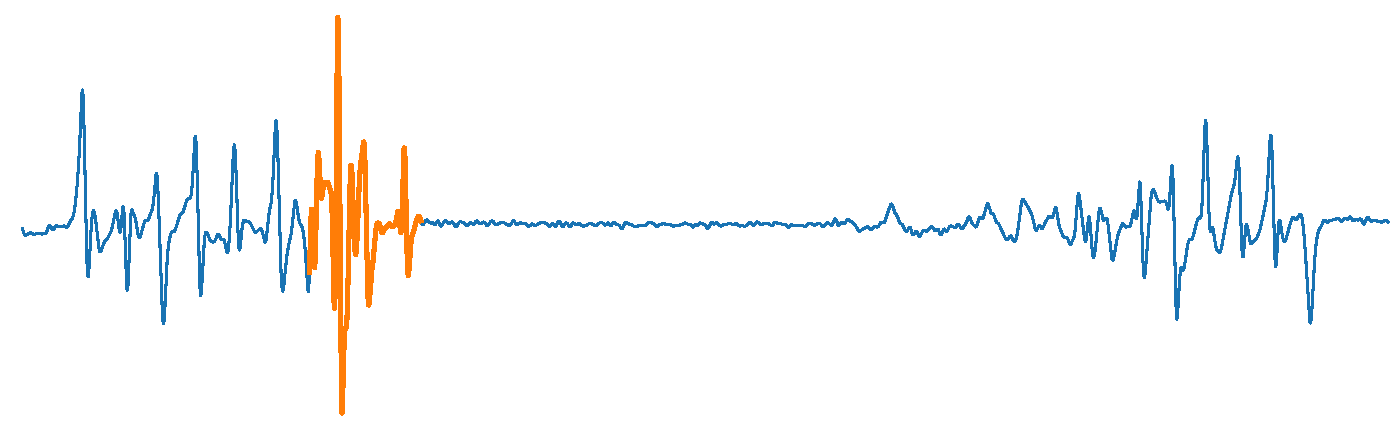
\includegraphics[width=0.55\linewidth, trim= 0 0 250 0, clip]{ex_signal_chute_2_epure.pdf}};
    \draw[color=gray!90,  line width=0.5pt] (-2.5,-2.1) rectangle (-0.5,2.2);
    \coordinate (A) at (-1.6,-2.5);
    \draw[->, >=stealth] (A) -- (-4.4,-4);
    \draw[->, >=stealth] (A) -- (-1.6,-4);
    \draw[->, >=stealth] (A) -- (1.2,-4);
    \draw (-5.5,-4.9) node[right]{$s$};
    \draw (-3.5,-4.9) node[right]{$\frac{d}{dt}s$};
    \draw (-0.5,-4.9) node[right]{$\mathcal{F}(s)$};
    \draw[->, >=stealth] (-1.6,-5.8) -- (-1.6,-6.5)
node[midway,below,yshift=-3pt]{\small Min, Max, Energy...};
    \path[draw,decorate,decoration=brace] (4.5,-7.5) -- (-7.5,-7.5)
node[midway,below,yshift=-3pt]{$\mathbf{x} \in \RR^{87}$};
    \end{tikzpicture}%
    }%
    \only<2->{%
    \begin{tikzpicture}[line cap=round,line join=round,>=triangle 45,x=0.2cm,y=0.4cm]
    \node[inner sep=0pt] at (0,0)
        {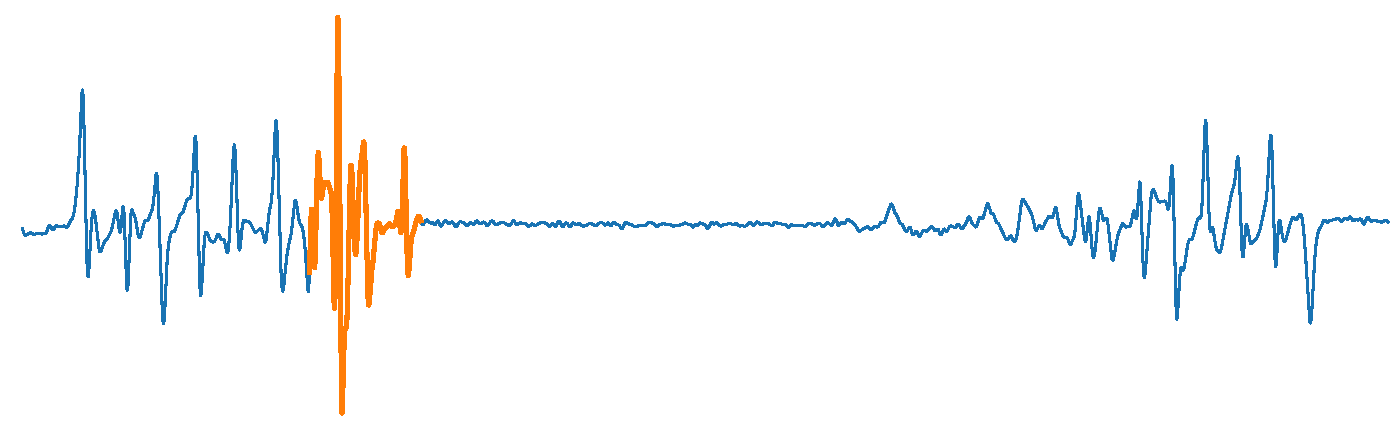
\includegraphics[width=0.55\linewidth, trim= 0 0 250 0, clip]{ex_signal_chute_2_epure.pdf}};
    \draw[color=gray!90,  line width=0.5pt] (-2.5,-2.1) rectangle (-0.5,2.2);
    \coordinate (A) at (-1.6,-2.5);
    \draw[->, >=stealth] (A) -- (-1.6,-3.5);
    \draw (-3.5,-4) node[right]{$x \in \RR^{87}$};
    \end{tikzpicture}
    }%
    \end{overlayarea}
    
    \vspace{3cm}
    \pause[3]
    \begin{enumerate}
        \item[3.] Classification model: Random Forest \cite{Breiman2001}, based on \textbf{decision trees}
        
%     \textbf{Random Forest}: Aggregation of \textbf{decision trees}.
    \end{enumerate}
\end{minipage}\hfill
\begin{minipage}[t]{0.49\linewidth}
    \vspace{0pt}
    \begin{tcolorbox}[title=Decision tree,size=title,boxrule=0.2pt]
    \small
    Feature space $\XX = \RR^Q$.
    Division of $\XX$ into non-overlapping regions $R_1,...,R_J$.
    Algorithm CART: recursive binary splits \cite{breiman84} that solve:
    \begin{gather*}
        \argmin_{X_{q}, \tau} \IG\;, \\
        \text{with} \quad \IG(X_{q}, \tau) = I(n) - \frac{N_{l}}{N_n}I(l) - \frac{N_{r}}{N_{n}}I(r)\;,\\
        \text{and} \quad I(n) = \mathrm{Gini}(n) = \sum_{k}p_{nk}(1-p_{nk})\;.
    \end{gather*}
    \end{tcolorbox}
    \begin{minipage}[t]{0.49\linewidth}
        \vspace{-5pt}
        \centering
        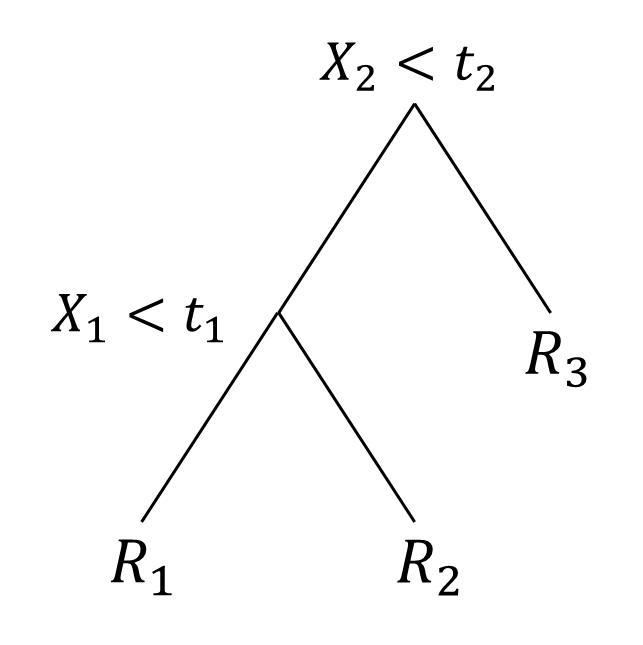
\includegraphics[width=0.65\linewidth, trim= 0 0 0 0, clip]{schema_decision_tree_1.png}\\
%     {\small Tree}
    \end{minipage}
    \begin{minipage}[t]{0.49\linewidth}
        \vspace{-5pt}
        \centering
        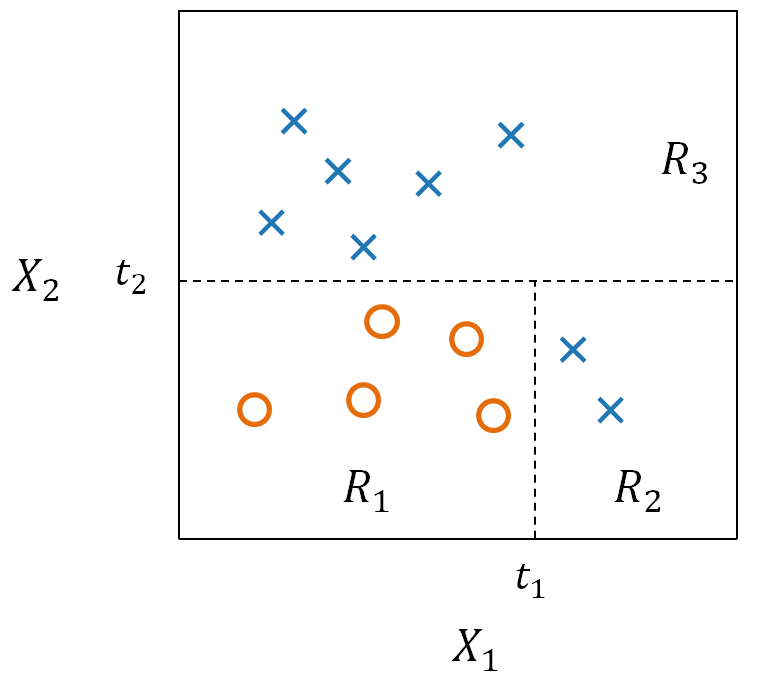
\includegraphics[width=0.9\linewidth, trim= 0 0 0 0, clip]{schema_decision_tree_3.png}\\
%     {\small Regions}
    \end{minipage}
    \centering
    \small
    Predicion function:\;
    $f(x) = \sum_{j=1}^{J}c_{j}\mathbbm{1}(x\in R_{j})$

\end{minipage}
\end{frame}

\begin{frame}{Fall detection}{Method}
\begin{minipage}[t]{0.4\linewidth}
    \vspace{0pt}
    \begin{tcolorbox}[title=Random forest,size=title,boxrule=0.2pt]
        Decision trees $d_1,...,d_{N_T}$ grown with two rules:
        \begin{itemize}
            \item Each tree is trained with a \emph{bootstrap} of the training set
            \item At each split, access to a random subset of pool of features
        \end{itemize}
        Each tree is a ``vote'' for a class.
        The prediction function is then
        \begin{gather*}
        f(x) = \argmax_{k}f_{k}(x)\;,\\
        \text{with} \quad f_{k}(x) = \frac{1}{N_T}\sum_{i=1}^{N_T}\mathbbm{1}(d_i(x)=k)
        \end{gather*}
    \end{tcolorbox}
\end{minipage}\hfill
\begin{minipage}[t]{0.58\linewidth}
    \vspace{0pt}
%     \medskip
    \renewcommand{\ratio}{0.5}
    \begin{overlayarea}{\linewidth}{3.4cm} %{width}{height}
%     \begin{overprint}
        \only<1>{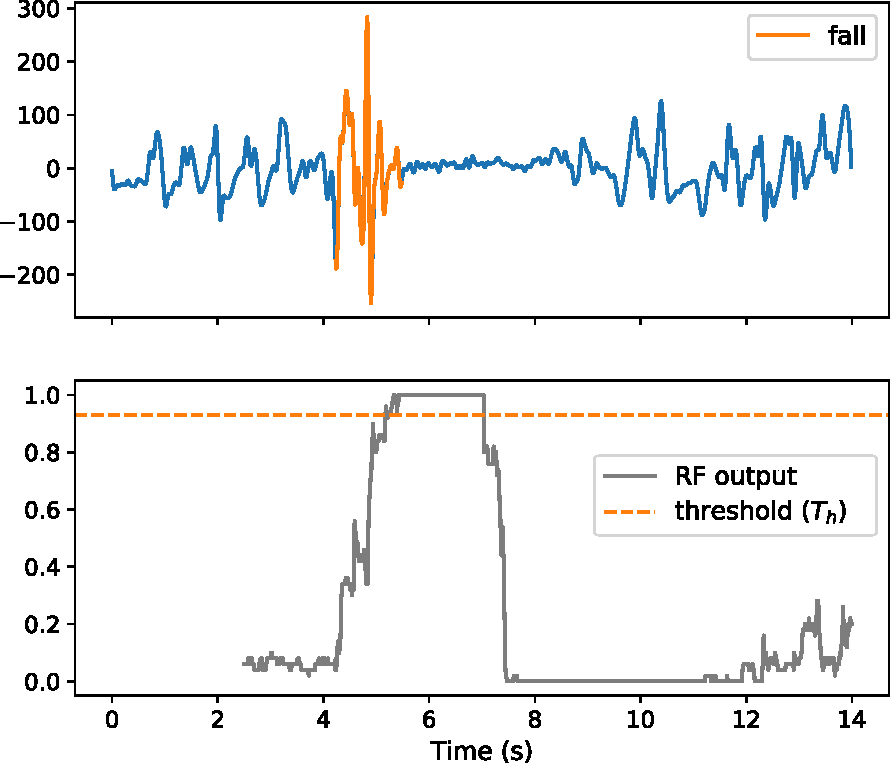
\includegraphics[width=\ratio\linewidth]{20140925a-1101-1115-FallLateral-Lateral-Yamina_begin_423_end_549_RFresponse_TP_beforebuff.pdf}}
        \only<1>{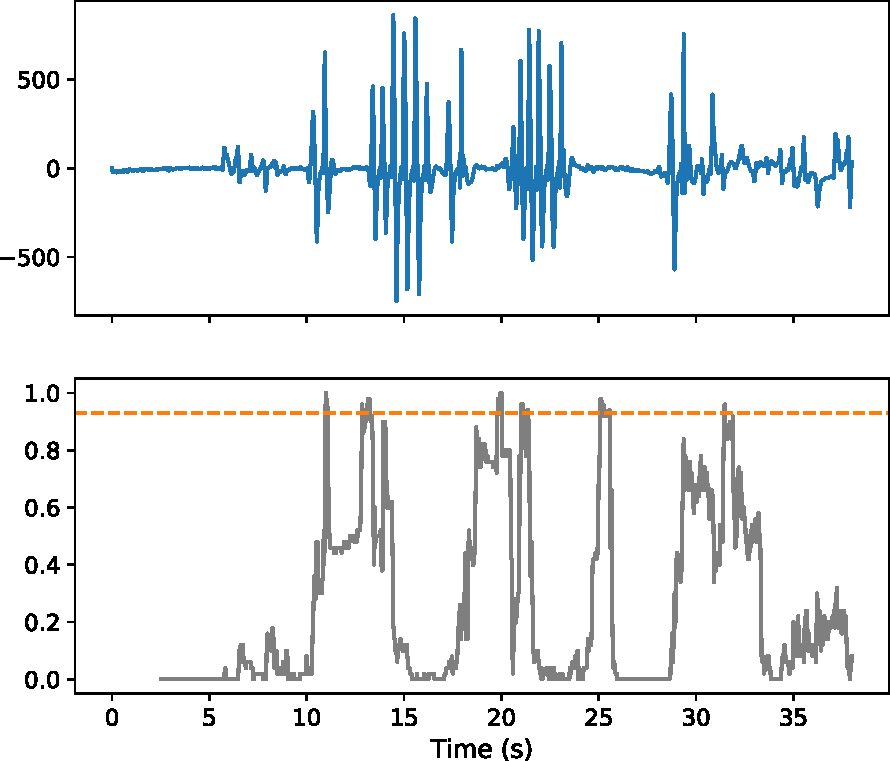
\includegraphics[width=\ratio\linewidth]{20140925a-0905-0943-Jump1-Yamina_RFresponse_TN_beforebuff_noleg.pdf}}
        \only<2->{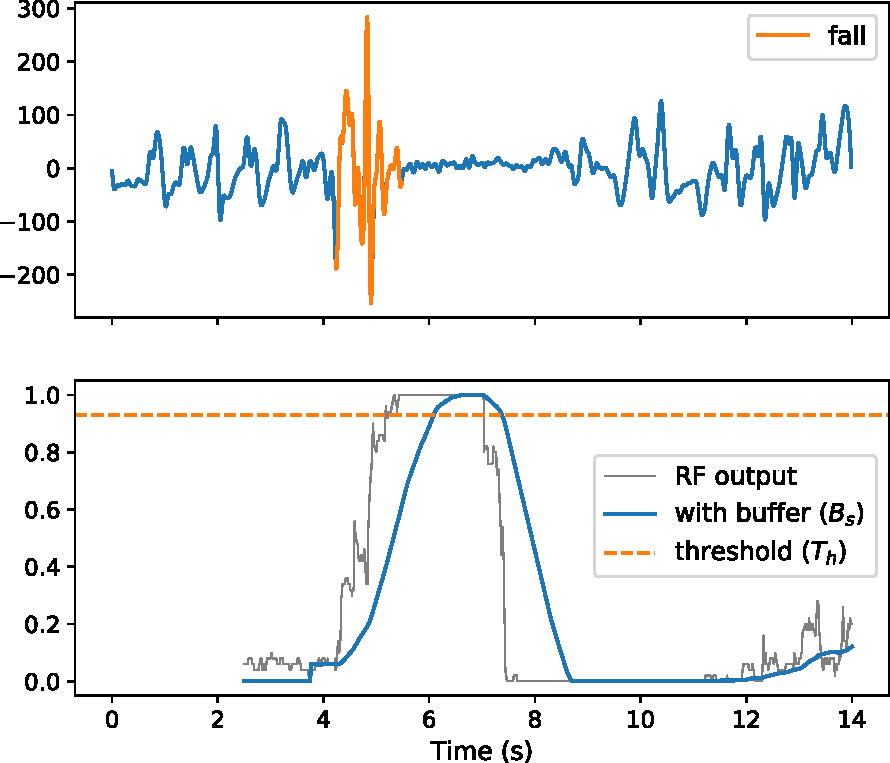
\includegraphics[width=\ratio\linewidth]{20140925a-1101-1115-FallLateral-Lateral-Yamina_begin_423_end_549_RFresponse_TP.pdf}}
        \only<2->{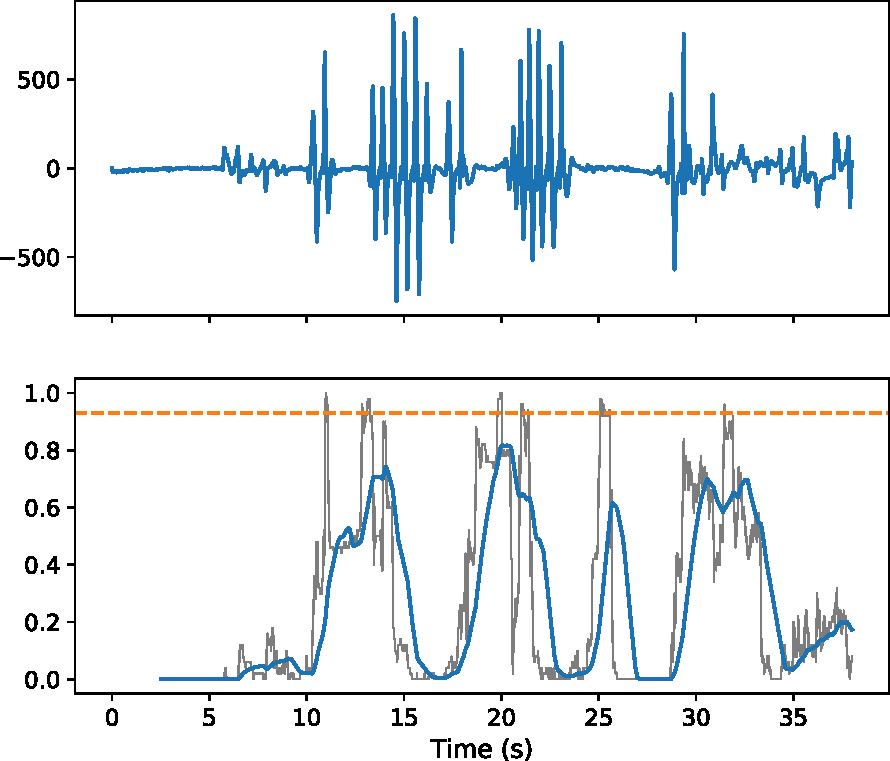
\includegraphics[width=\ratio\linewidth]{20140925a-0905-0943-Jump1-Yamina_RFresponse_TN.pdf}}
    \end{overlayarea}
%     \end{overprint}
    
    \textbf{Time aggregation}
    
    $N_f(t)$ : number of trees voting for \emph{fall}\\
    Use a buffer $B_s \in \NN$ and a threshold $T_h \in [0, 1]$
    \begin{gather*}
    g(t) = \frac{\sum\limits_{u=t-B_{s}+1}^{t}N_{f}(u)}{B_{s}\times N_{T}}\\
    \text{New binary classification function:} \quad
    d(t) = 
    \begin{cases}
    1, & \textit{if}\ g(t) > T_{h} \\
    0, & \textit{otherwise}
    \end{cases}
    \end{gather*}
\end{minipage}



\end{frame}

\begin{frame}{Fall detection}{Method}

\begin{minipage}[t]{0.49\linewidth}
    \vspace{0pt}
    \textbf{Data augmentation}\\
    Select $r$ windows in training signals

    \begin{tikzpicture}[line cap=round,line join=round,>=triangle 45,x=0.2cm,y=0.4cm]
    \node[inner sep=0pt] at (0,0)
        {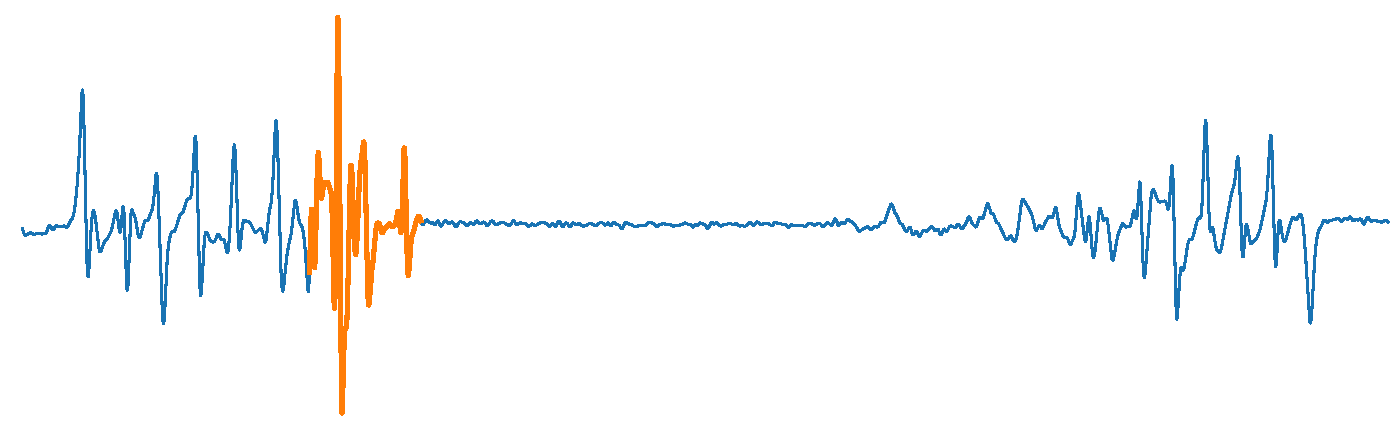
\includegraphics[width=0.55\linewidth, trim= 0 0 250 0, clip]{ex_signal_chute_2_epure.pdf}};
    \onslide<1>\draw[color=gray!90,  line width=0.5pt] (-3.3,-2.1) rectangle (-0.5,2.2);
    \onslide<2>\draw[color=gray!90,  line width=0.5pt] (-2.5,-2.1) rectangle (0.3,2.2);
    \onslide<3->\draw[color=gray!90,  line width=0.5pt] (-2.9,-2.1) rectangle (-0.1,2.2);
%     \draw (-2.5,-2.5) node[right]{$\mathbf{x} \in \RR^{87}$};
    \end{tikzpicture}

    \begin{overlayarea}{\linewidth}{1.2cm}
    \only<1-3>{
    $\left[
    \begin{array}{ccc}
        x_{1,1} & ... & x_{1,Q} \\
        \onslide<2-3>{x_{2,1} & ... & x_{2,Q}} \\
        \onslide<3>{x_{3,1} & ... & x_{3,Q}} \\
    \end{array}
    \right]
    $
    }
    \only<4->{
    $\left[
    \begin{array}{ccc}
        x_{1,1} & ... & x_{1,Q} \\
        \vdots & & \vdots \\
        x_{r,1} & ... & x_{r,Q} \\
    \end{array}
    \right]
    $
    }
    \end{overlayarea}
    
    \textbf{Feature reduction}
    \begin{gather*}
    \text{Tree: } I(T, X_{q}) = \sum_{t\in T}p(t)\Delta i(t)\mathbbm{1}(v(t)=X_{q})\\
    \text{Random forest: }I(X_{q}) = \frac{1}{N_{T}}\sum_{n=1}^{N_T}I(T_n, X_{q})
    \end{gather*}
    \begin{tcolorbox}[title=Recursive feature elimination,size=title,boxrule=0.2pt]
        \begin{enumerate}
            \item 
        \end{enumerate}
    \end{tcolorbox}

\end{minipage}\hfill
\begin{minipage}[t]{0.49\linewidth}
    \vspace{0pt}

\end{minipage}

\end{frame}
\begin{frame}{Fall detection}{Results}
\end{frame}

\section{Transfer learning}
\subsection{Operational data}
\begin{frame}{Transfer learning on decision tree}{Experimental vs. operational}
\begin{minipage}[t]{0.49\linewidth}
    \vspace{0pt}
    \textbf{Transfer learning}
    \begin{itemize}
        \item Source domain: $\mathcal{D}_{S} = \{\mathcal{X}_{S}, P(X_{S})\}$\\
        \item Target domain: $\mathcal{D}_{T} = \{\mathcal{X}_{T}, P(X_{T})\}$\\
        \item Source task: $\mathcal{T}_{S} = \{\mathcal{Y}_{S}, f^S\}$\\
        \item Target task: $\mathcal{T}_{T} = \{\mathcal{Y}_{T}, f^T\}$\\
    \end{itemize}
\end{minipage}
\begin{minipage}[t]{0.49\linewidth}
    \vspace{0pt}
    \textbf{Our case}
    \begin{itemize}%[label=$\bullet$]
        \item $\mathcal{X}_{S} = \mathcal{X}_{T}$
        \item \textcolor{myorange}{$P(X_{S}) \neq P(X_{T})$}
        \item $\mathcal{Y}_{S} = \mathcal{Y}_{T}$
        \item \textcolor{myorange}{$f^S \neq f^T$}
    \end{itemize}
\end{minipage}

\bigskip

\renewcommand{\ratio}{0.32}
\begin{minipage}[t]{\linewidth}
    \centering
    \begin{minipage}[t]{\ratio\linewidth}
        \centering
        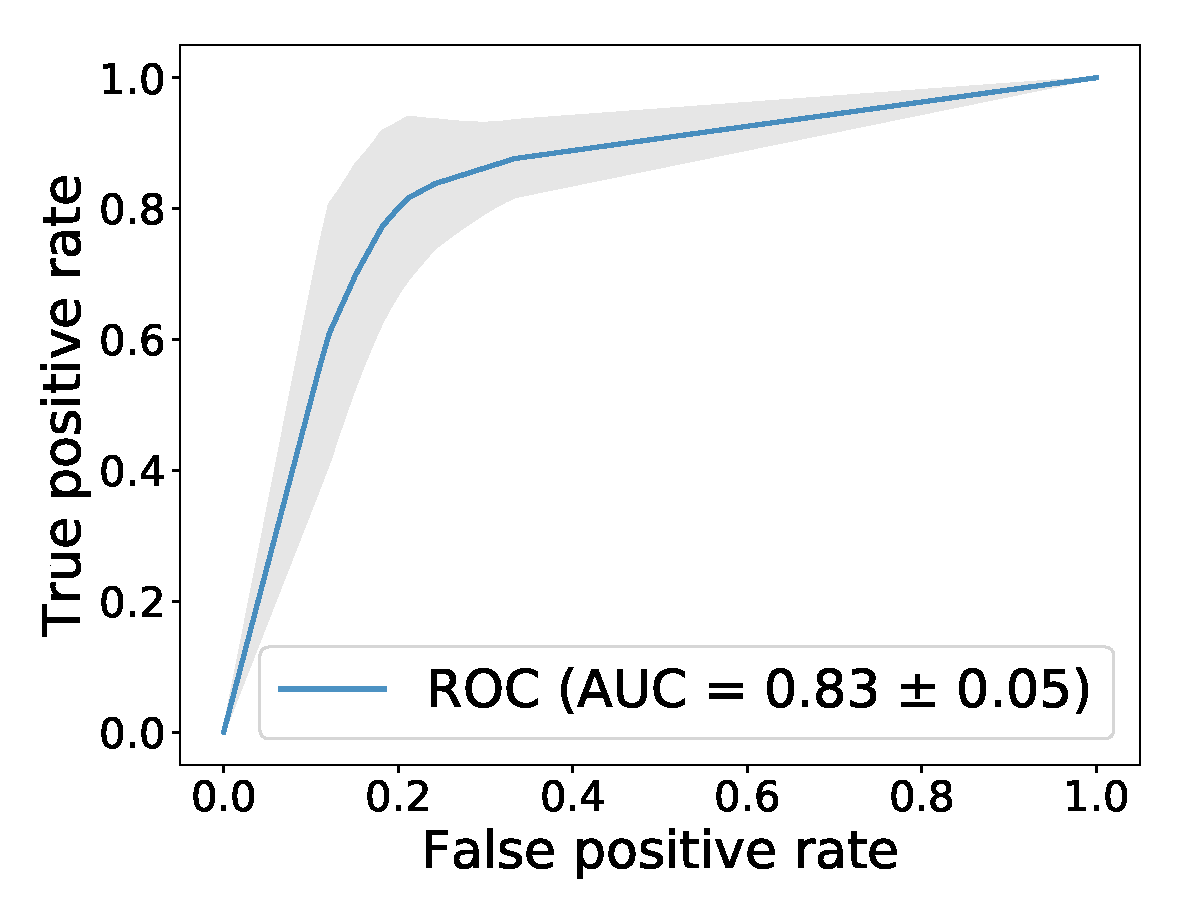
\includegraphics[width=\linewidth]{kfold_10_ntree_1_featmat_base_ech1nb_feat_872019_11_25RF_Source_On_Source_ROC.pdf}\\
        {\small \emph{Source} tested on source}
    \end{minipage}
    \begin{minipage}[t]{\ratio\linewidth}
        \centering
        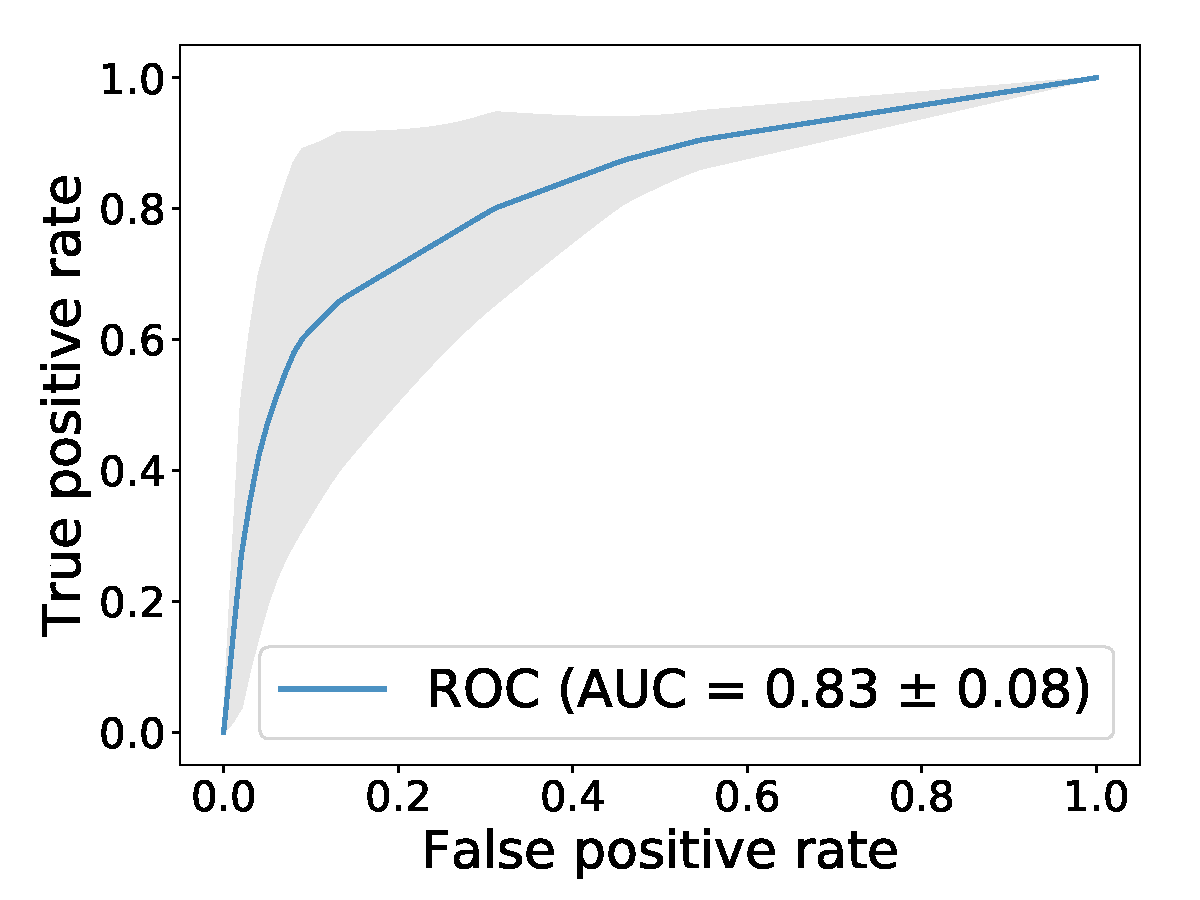
\includegraphics[width=\linewidth]{kfold_10_ntree_1_featmat_base_ech1nb_feat_872019_11_25RF_Source_On_Target_ROC.pdf}\\
        {\small \emph{Source} tested on target}
    \end{minipage}
    \begin{minipage}[t]{\ratio\linewidth}
        \centering
        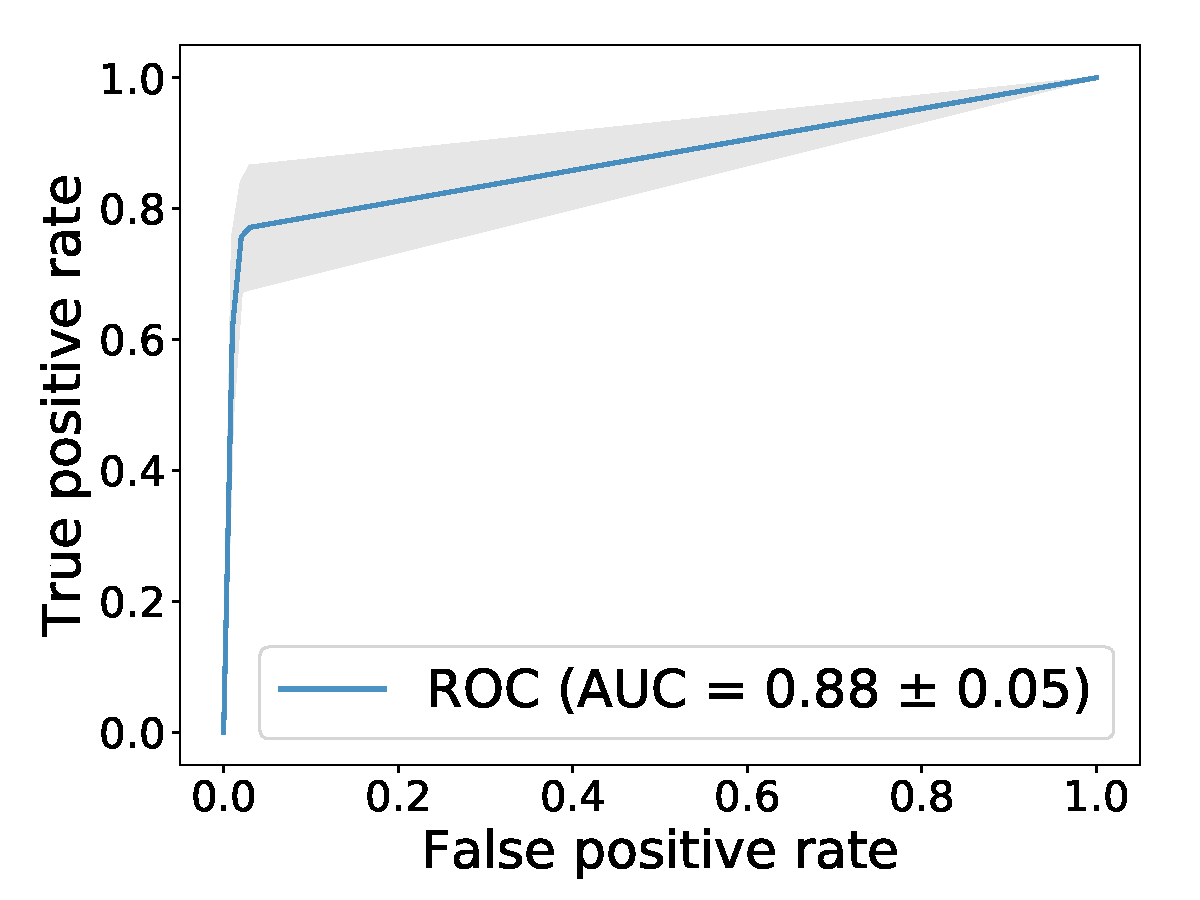
\includegraphics[width=\linewidth]{kfold_10_ntree_1_featmat_base_ech1nb_feat_872019_11_25RF_Target_On_Target_ROC.pdf}\\
        {\small \emph{Target} tested on target}
    \end{minipage}
\end{minipage}

\end{frame}

\begin{frame}{Transfer learning on decision tree}{Model-based transfer}
\begin{minipage}[t]{0.49\linewidth}
    \vspace{0pt}
    \centering
    \textbf{Structure Expansion / Reduction (SER)}
    
    \renewcommand{\ratio}{0.55}
%     \begin{overprint}
%         \onslide<1>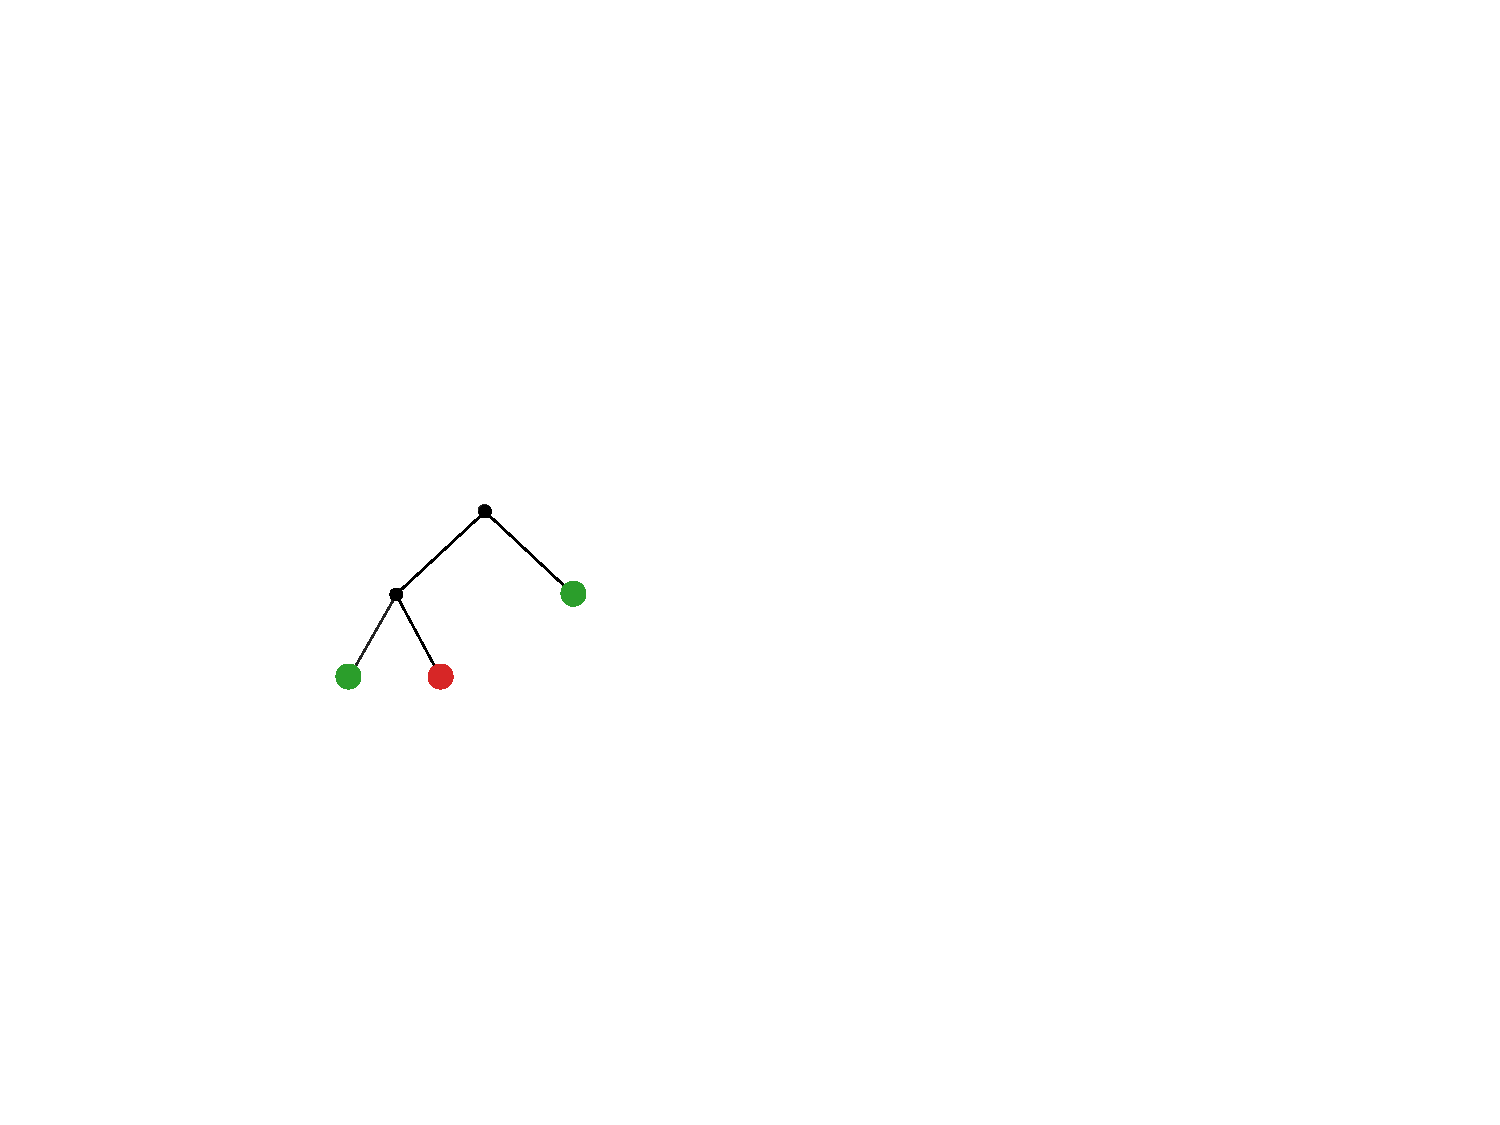
\includegraphics[width=\ratio\linewidth, trim={100 150 430 200}, clip]{ser_0.pdf}
%         \onslide<2>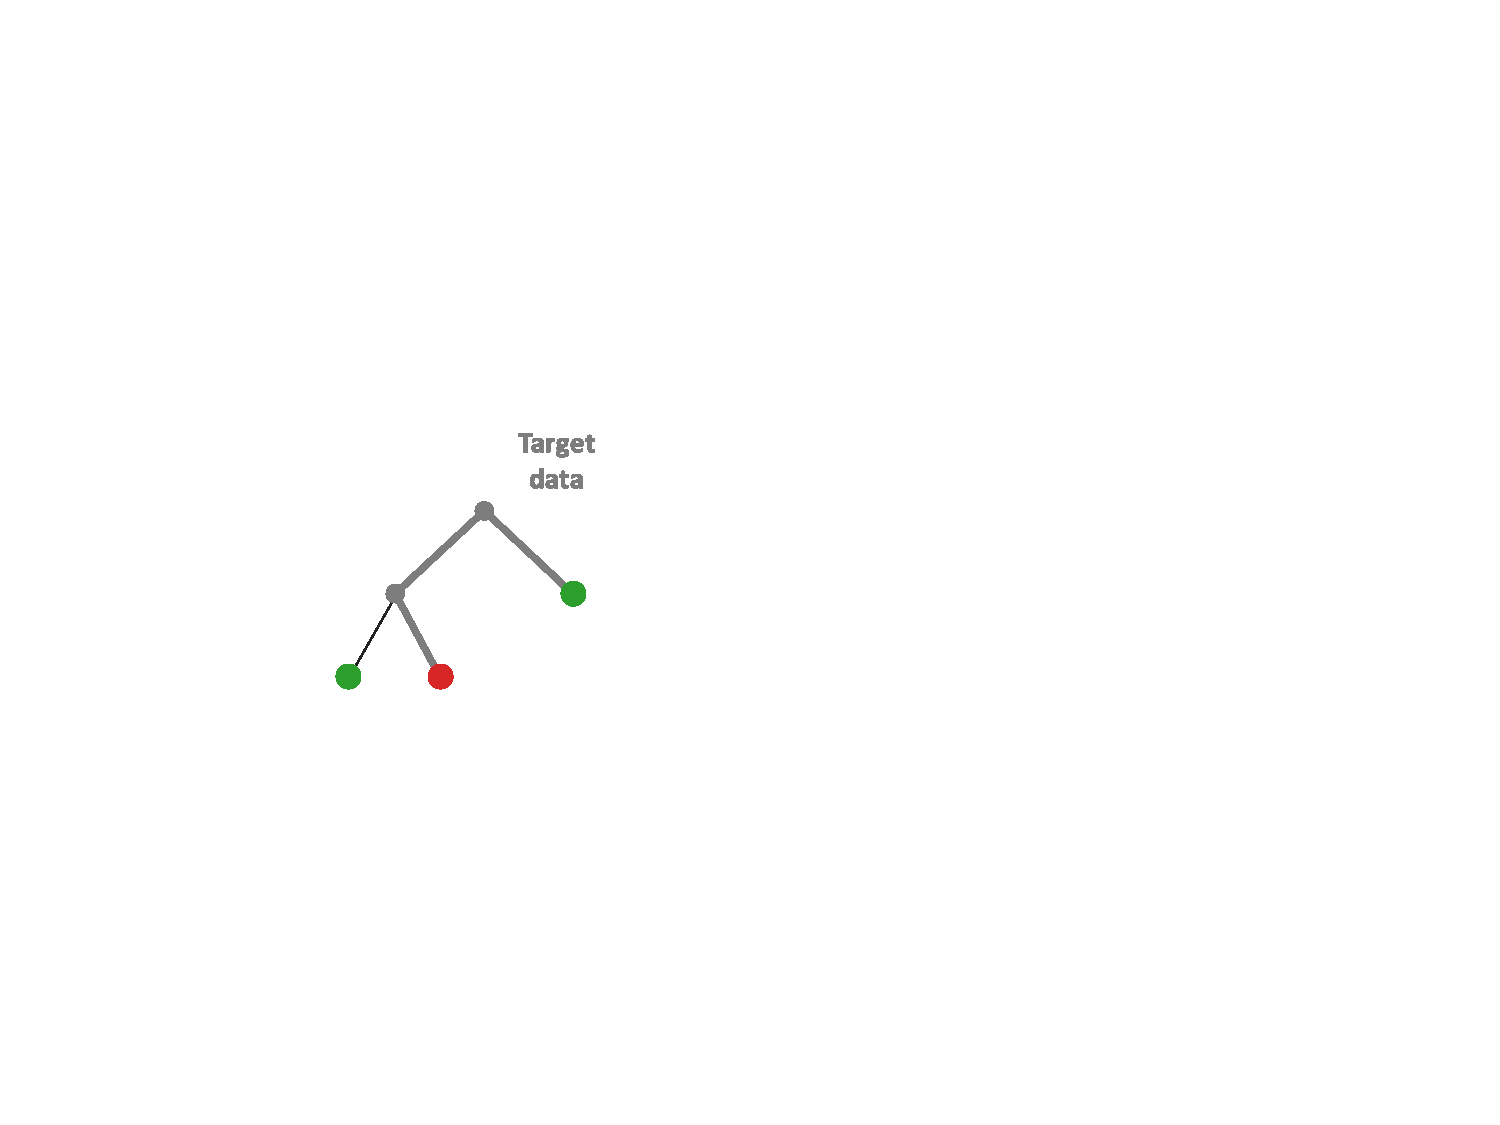
\includegraphics[width=\ratio\linewidth, trim={100 150 430 200}, clip]{ser_1.pdf}
%         \onslide<3>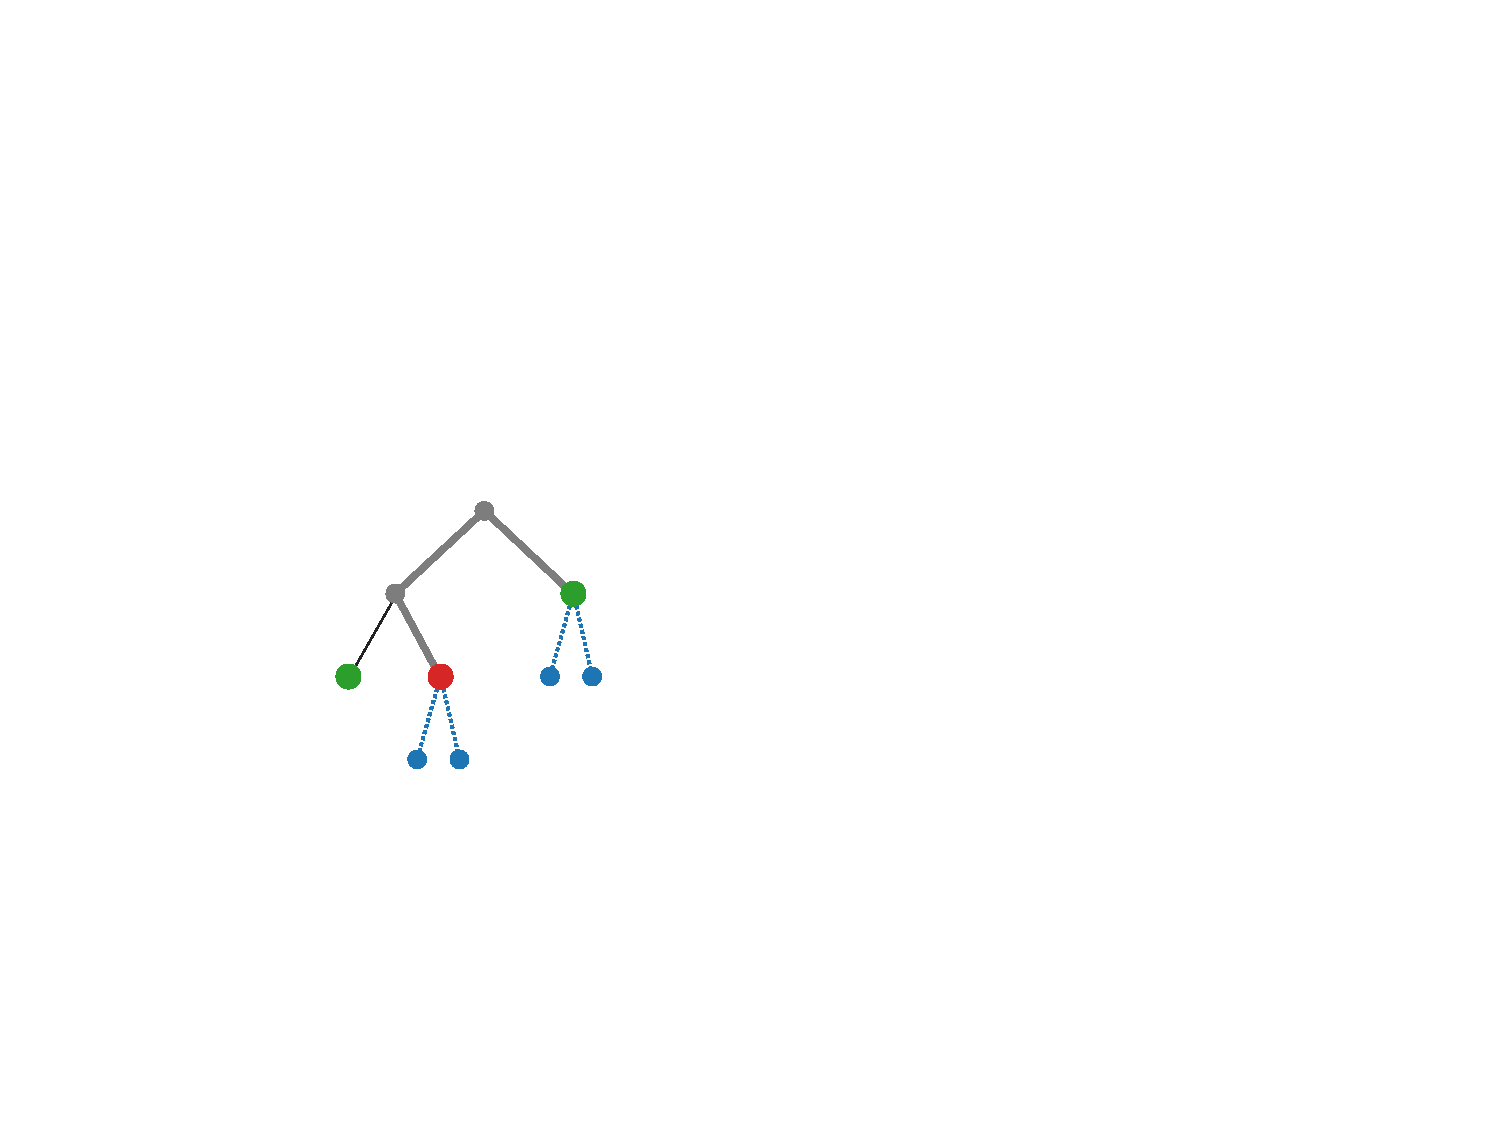
\includegraphics[width=\ratio\linewidth, trim={100 150 430 200}, clip]{ser_2.pdf}
%         \onslide<4>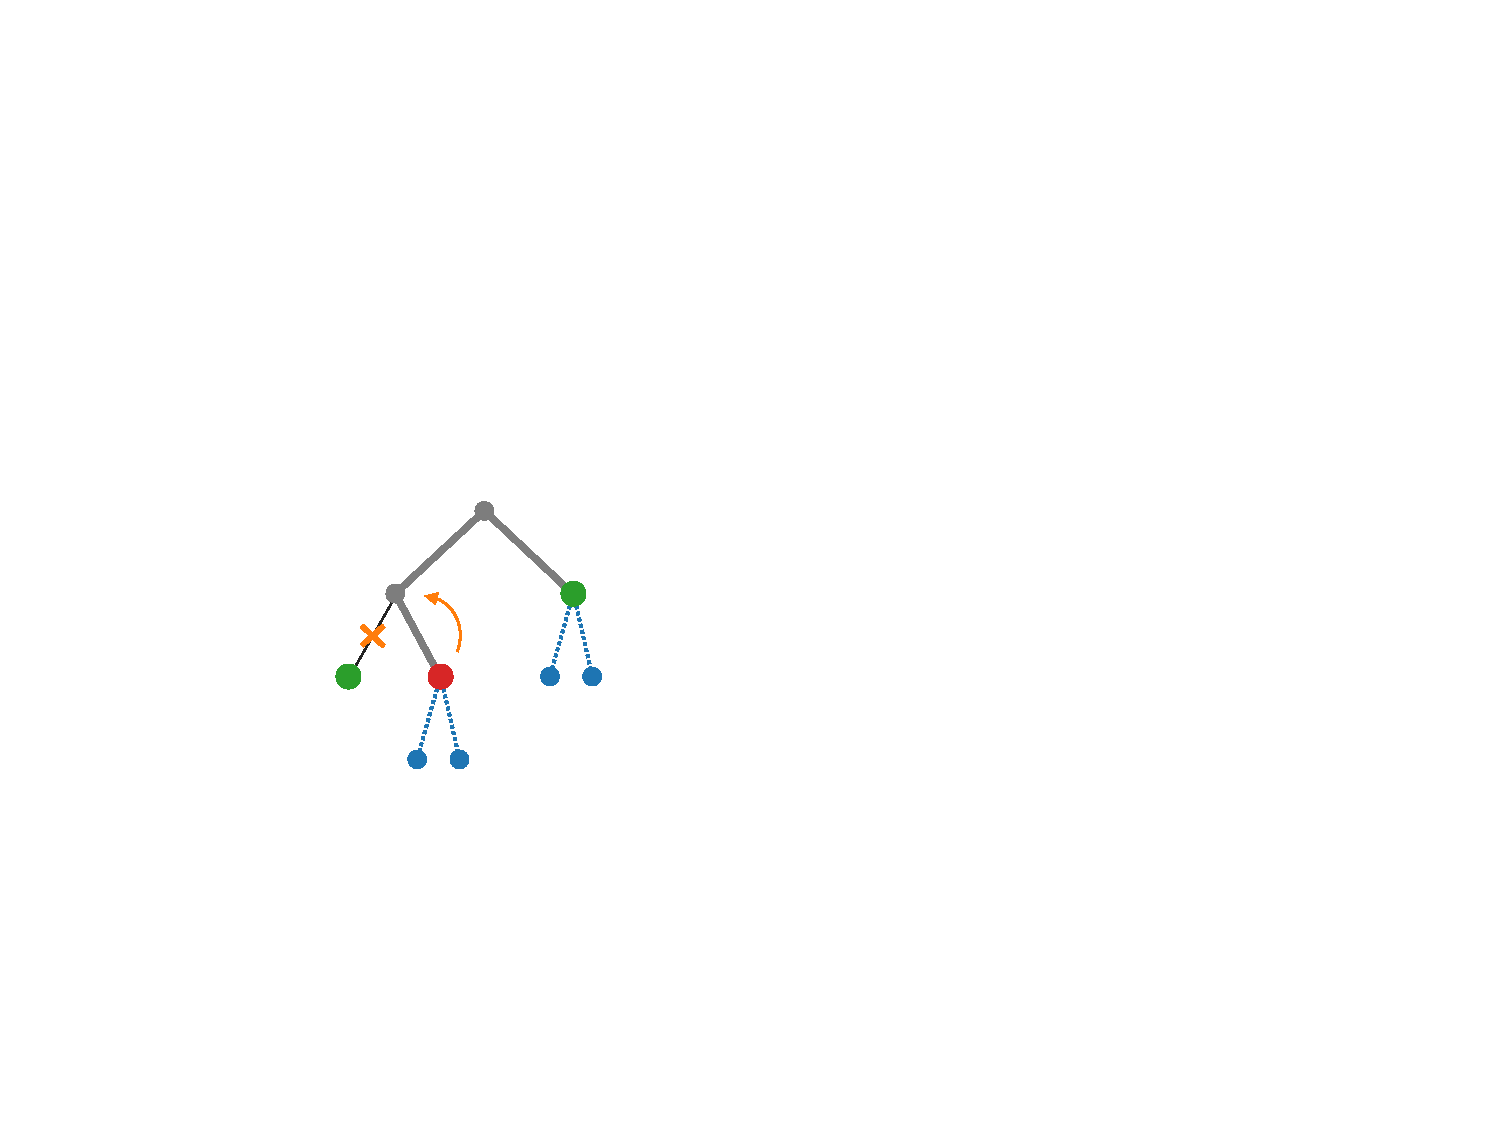
\includegraphics[width=\ratio\linewidth, trim={100 150 430 200}, clip]{ser_3.pdf}
%         \onslide<5->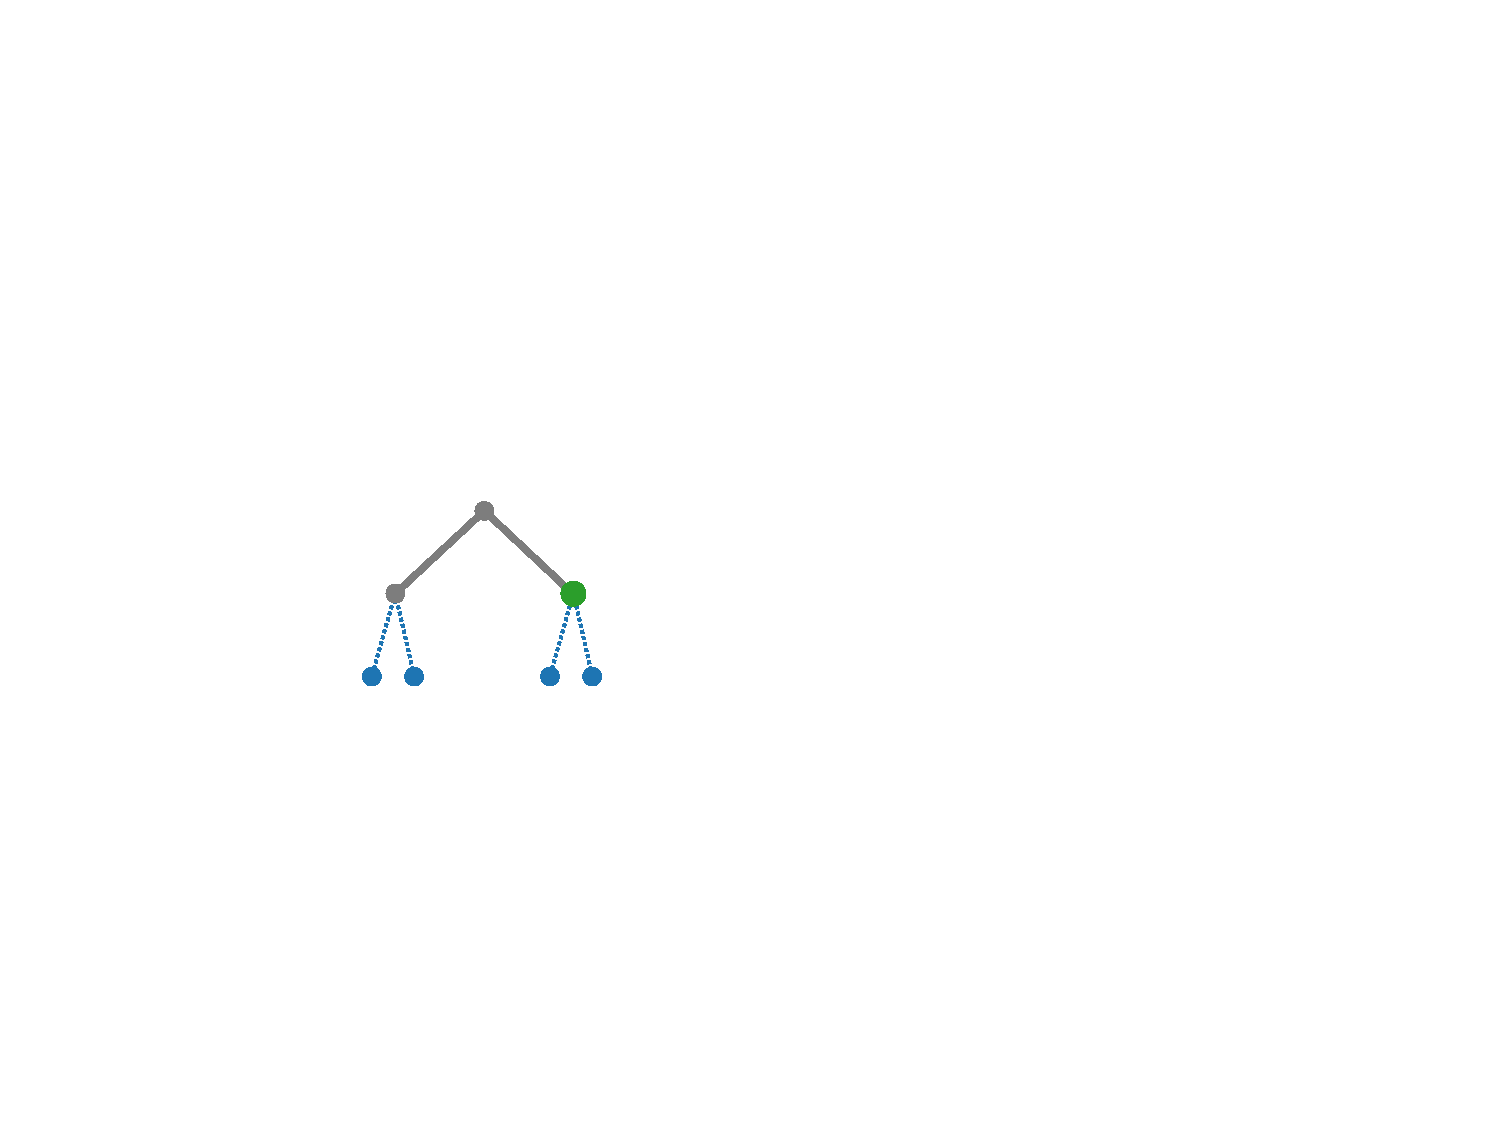
\includegraphics[width=\ratio\linewidth, trim={100 150 430 200}, clip]{ser_4.pdf}
%     \end{overprint}
    \begin{overprint}
        \onslide<1>\centering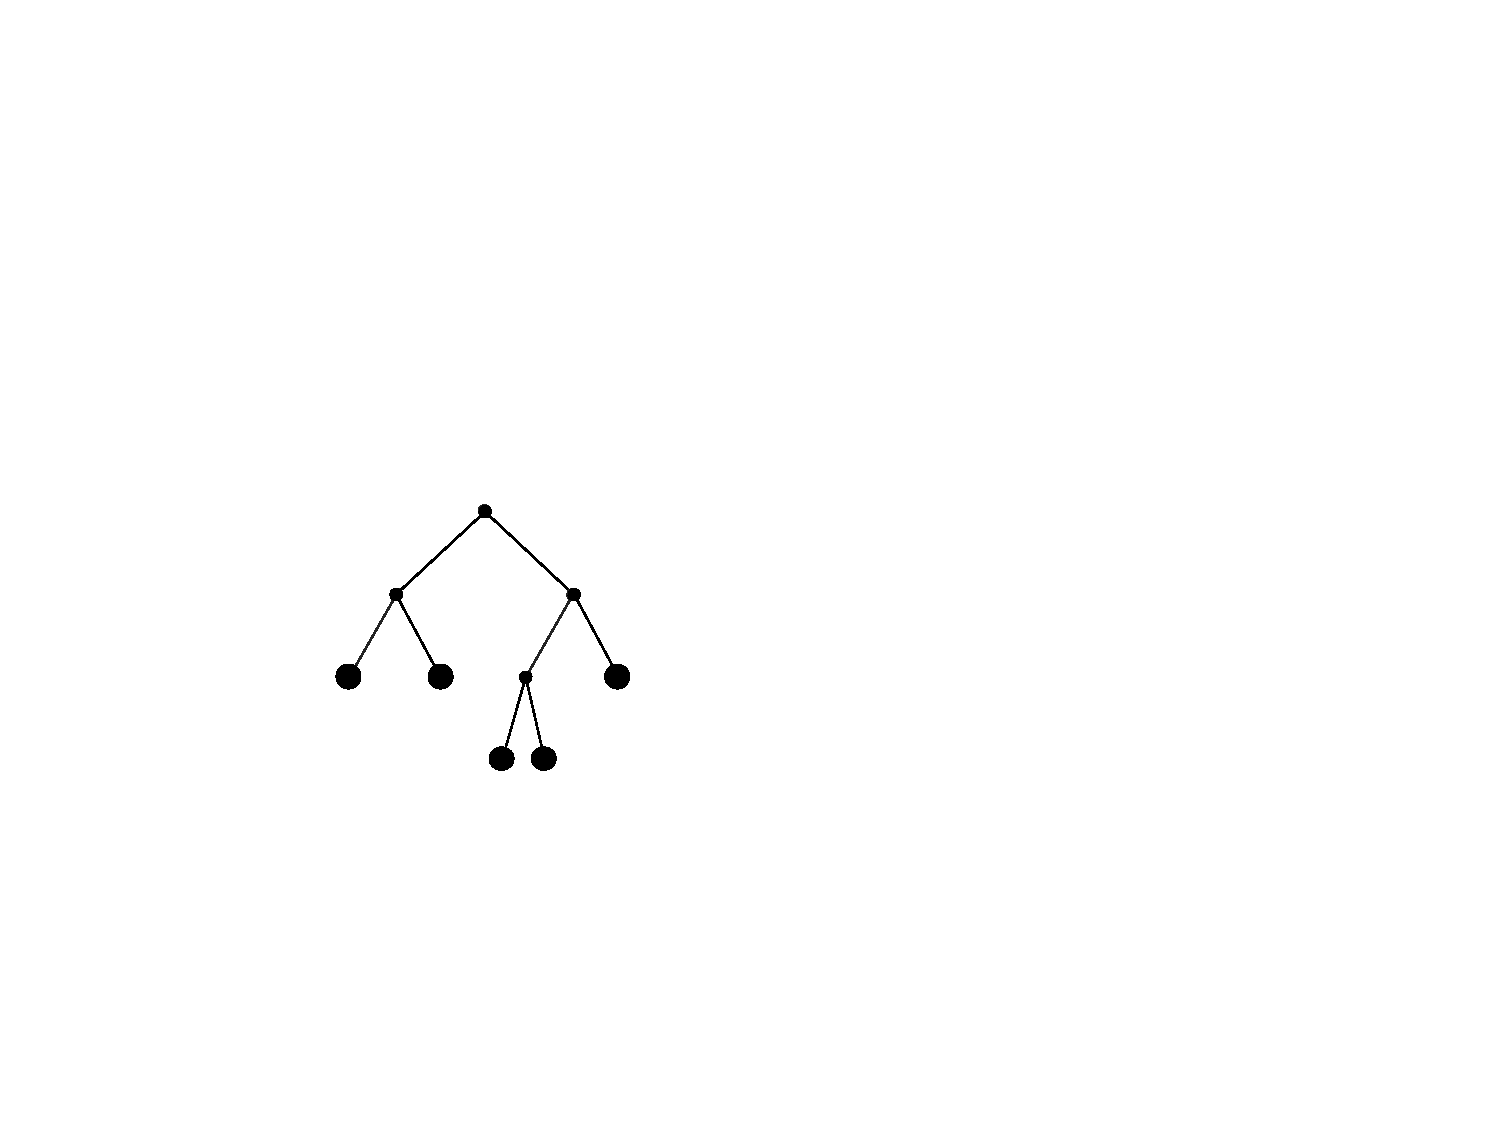
\includegraphics[width=\ratio\linewidth, trim={150 120 410 200}, clip]{schemas_ser_1.pdf}
        \onslide<2>\centering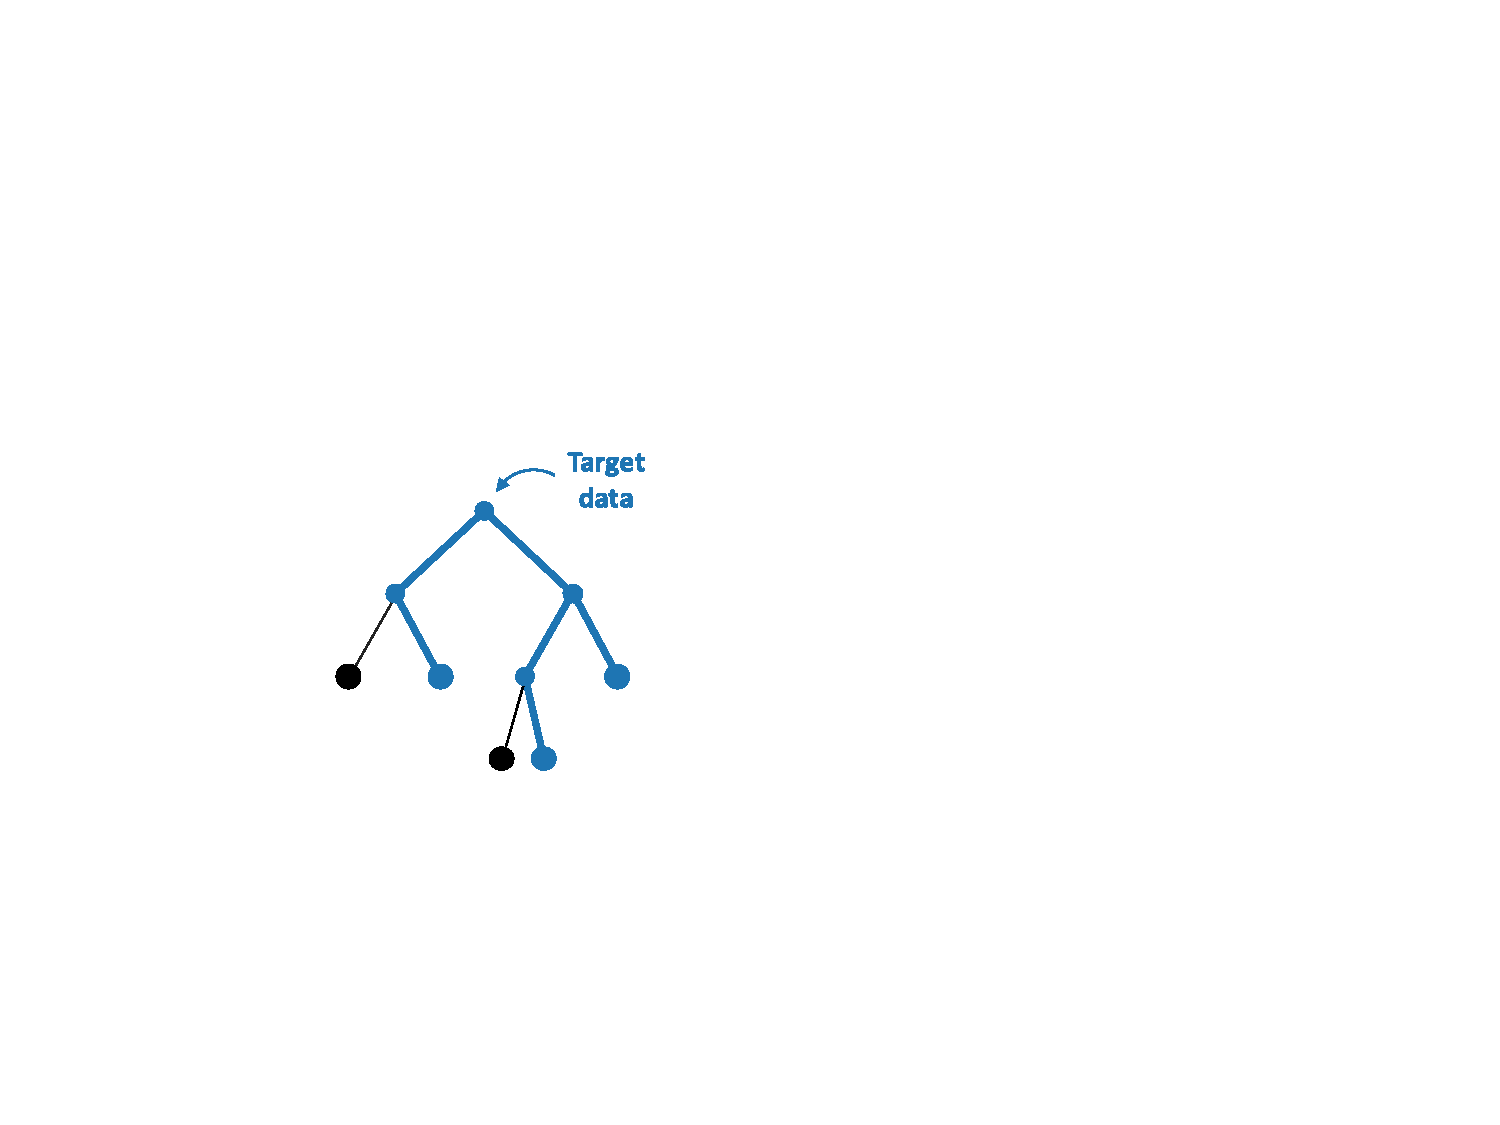
\includegraphics[width=\ratio\linewidth, trim={150 120 410 200}, clip]{schemas_ser_2.pdf}
        \onslide<3>\centering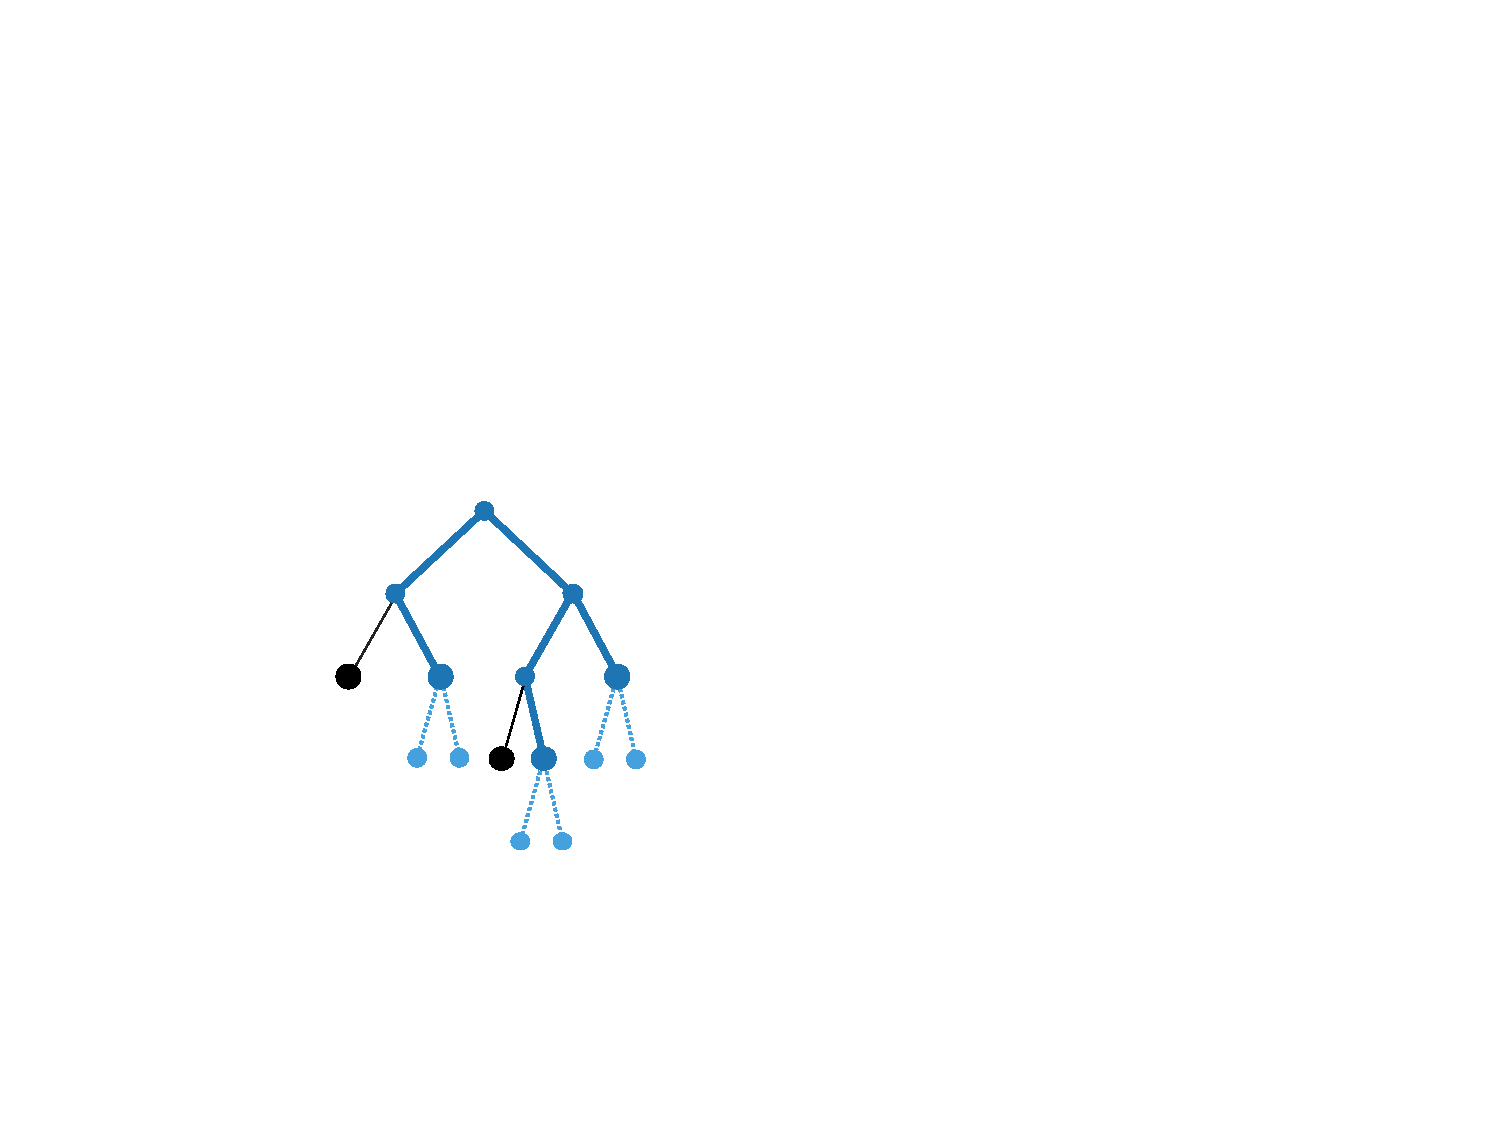
\includegraphics[width=\ratio\linewidth, trim={150 120 410 200}, clip]{schemas_ser_3.pdf}
        \onslide<4>\centering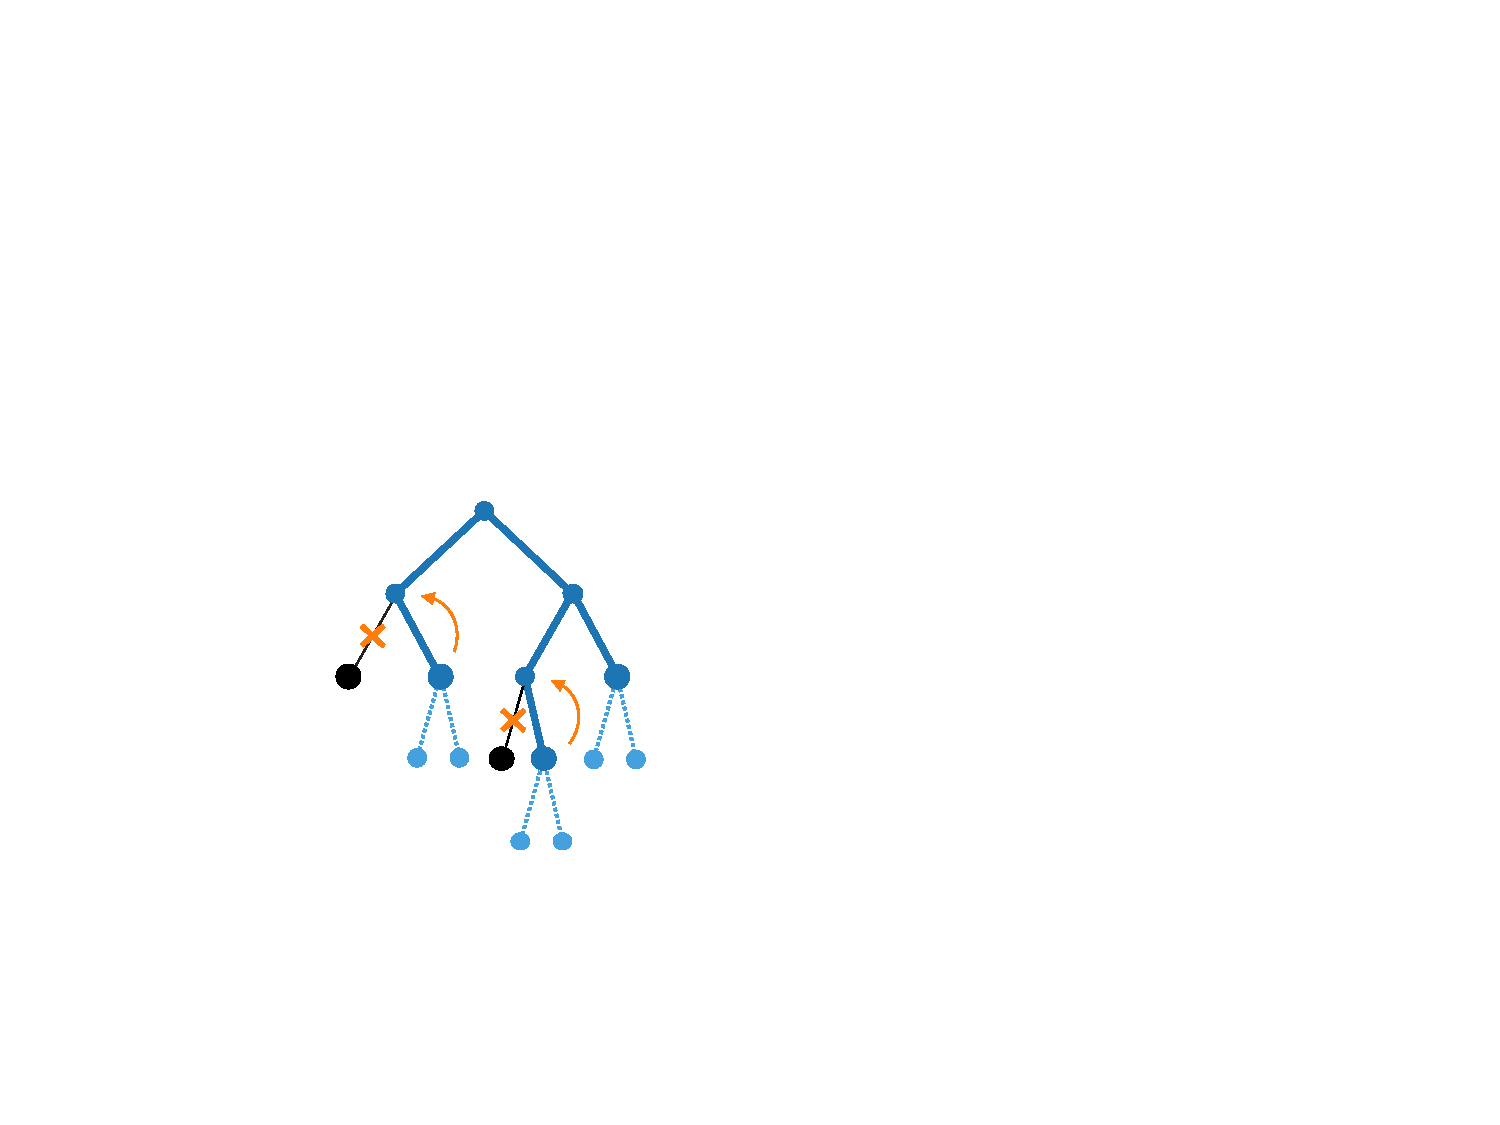
\includegraphics[width=\ratio\linewidth, trim={150 120 410 200}, clip]{schemas_ser_4.pdf}
        \onslide<5->\centering\includegraphics[width=\ratio\linewidth, trim={150 120 410 200}, clip]{schemas_ser_5.pdf}
    \end{overprint}
    
    \pause \pause
    \textcolor{myblue}{1. Expansion}\\
    \pause
    \textcolor{myorange}{2. Reduction}\\
    \bigskip
    \onslide<11->{Partition refinement or simplification}

\end{minipage}\hfill
\begin{minipage}[t]{0.49\linewidth}
    \vspace{0pt}
    \centering
    \textbf{Structure Transfer (STRUT)}
    
    \renewcommand{\ratio}{0.55}
%     \begin{overprint}
%         \onslide<6>\includegraphics[width=\ratio\linewidth, trim={100 180 430 200}, clip]{strut_0.pdf}
%         \onslide<7>\includegraphics[width=\ratio\linewidth, trim={100 180 430 200}, clip]{strut_1.pdf}
%         \onslide<8>\includegraphics[width=\ratio\linewidth, trim={100 180 430 200}, clip]{strut_2.pdf}
%         \onslide<9>\includegraphics[width=\ratio\linewidth, trim={100 180 430 200}, clip]{strut_3.pdf}
%         \onslide<10->\includegraphics[width=\ratio\linewidth, trim={100 180 430 200}, clip]{strut_4.pdf}
%     \end{overprint}
    \begin{overprint}
        \onslide<6>\centering\includegraphics[width=\ratio\linewidth, trim={140 150 410 200}, clip]{schemas_strut_1_15.pdf}
        \onslide<7>\centering\includegraphics[width=\ratio\linewidth, trim={140 150 410 200}, clip]{schemas_strut_2_15.pdf}
        \onslide<8>\centering\includegraphics[width=\ratio\linewidth, trim={140 150 410 200}, clip]{schemas_strut_3_15.pdf}
        \onslide<9>\centering\includegraphics[width=\ratio\linewidth, trim={140 150 410 200}, clip]{schemas_strut_4_15.pdf}
        \onslide<10->\centering\includegraphics[width=\ratio\linewidth, trim={140 150 410 200}, clip]{schemas_strut_5_15.pdf}
    \end{overprint}
    \onslide<8->
    \textcolor{myorange}{1. Pruning}\\
    \onslide<10->
    \textcolor{myblue}{2. Threshold update}\\
    \bigskip
    \onslide<11->
    Drifts
\end{minipage}

\cite{segev2017learn}

\end{frame}

\begin{frame}{Transfer learning on decision tree}{Leaf loss risk}

\begin{minipage}[t]{0.38\textwidth}
    \vspace{0pt}
    \begin{tcolorbox}[title=Homogeneous class imbalance,size=title,boxrule=0.2pt]
    \begin{align*}
        & P^T(x|y) = P^S(x|y) \\
        & P^T(y|x) = \lambda_y \frac{P^S(y|x)}{\int{\lambda_y P^S(y|x)dy}}
    %       & \textrm{with} \quad \lambda_y = \frac{P_y^T}{P_y^S} 
    \end{align*}
        $\text{with} \quad \lambda_y = \frac{P^T(y)}{P^S(y)}$
    \end{tcolorbox}
\end{minipage}\hfill
\begin{minipage}[t]{0.59\textwidth}
    \vspace{0pt}
    \pause
    \begin{tcolorbox}[title=Leaf loss risk,size=title,boxrule=0.2pt]
            Significant leaf: Leaf $l$ that conserves the minority class $k_{min}$ after Target update:
        \begin{equation*}
        \forall k \neq k_{min},\quad {P}^T(y = k_{min} \,|\, x \in l) > {P}^T(y = k \,|\, x \in l) 
        \label{eqF_rep_targ}
        \end{equation*}
        Leaf loss risk:
        \begin{equation*}
        R_{L}(l)={P}^T(x \notin l \,|\, y = k_{min})^{n_{k_{min}}} 
        \label{eq_risk_value}
        \end{equation*}
    \end{tcolorbox}
\end{minipage}
\pause
\begin{tcolorbox}[title=Leaf loss risk under homogeneous class imbalance,size=title,boxrule=0.2pt]
    \begin{equation*}
    \forall k \neq k_{min}, \quad \lambda_{k_{min}}  {P}^S(y = k_{min} \,|\, x \in l) > \lambda_k  {P}^S(y = k \,|\, x \in l)
    \end{equation*}
    \begin{equation*}
    R_{L}(l)={P}^S(x \notin l \,|\, y = k_{min})^{n_{k_{min}}}
    \end{equation*}
\end{tcolorbox}

\end{frame}

\begin{frame}{Transfer learning on decision tree}{Leaf loss risk}
\renewcommand{\ratio}{0.78}
\renewcommand{\ratiob}{0.45}
    \centering
    \begin{minipage}[t]{0.8\linewidth}\vspace{0pt}
        \centering
        \begin{minipage}[t]{\ratiob\linewidth}\vspace{0pt}
            \centering
            \includegraphics[width=\ratio\linewidth]{leaf_loss_NTarget200_Lambda1.pdf}\\
            {\small(a)\; Balanced data with 200 instances}
        \end{minipage}\vspace{0.2cm}
        \begin{minipage}[t]{\ratiob\linewidth}\vspace{0pt}
            \centering
            \includegraphics[width=\ratio\linewidth]{leaf_loss_NTarget100_Lambda1.pdf}\\
            {\small(b)\; Balanced data with 100 instances }
        \end{minipage}
        % \hfill
        \\
        \begin{minipage}[t]{\ratiob\linewidth}\vspace{0pt}
            \centering
            \includegraphics[width=\ratio\linewidth]{leaf_loss_NTarget200_Lambda01.pdf}\\
            {\small (c)\; Imbalanced data (10\% ratio) with 200 instances}
        \end{minipage}
        \centering
        \begin{minipage}[t]{\ratiob\linewidth}\vspace{0pt}
            \centering
            \includegraphics[width=\ratio\linewidth]{leaf_loss_NTarget100_Lambda01.pdf}\\
            {\small (d)\; Imbalanced data (10\% ratio) with 100 instances}
        \end{minipage}\vspace{0.1cm}
    \end{minipage}

\end{frame}

\begin{frame}{Transfer learning on decision tree}{SER for class imbalance}
\begin{minipage}[t]{0.49\linewidth}
    \vspace{0pt}
    
    \centering
    \textbf{Structure Expansion and controlled Reduction}\\
        
    \renewcommand{\ratio}{0.8}
    \begin{overprint}
        \onslide<1>\includegraphics[width=\ratio\linewidth, trim={100 120 390 200}, clip]{schemas_ser_1.pdf}
        \onslide<2>\includegraphics[width=\ratio\linewidth, trim={100 120 390 200}, clip]{schemas_sernr_1_15.pdf}
        \onslide<3>\includegraphics[width=\ratio\linewidth, trim={100 120 390 200}, clip]{schemas_sernr_2_15.pdf}
        \onslide<4>\includegraphics[width=\ratio\linewidth, trim={100 120 390 200}, clip]{schemas_sernr_3_15.pdf}
        \onslide<5>\includegraphics[width=\ratio\linewidth, trim={100 120 390 200}, clip]{schemas_sernr_4_15.pdf}
        \onslide<6>\includegraphics[width=\ratio\linewidth, trim={100 120 390 200}, clip]{schemas_sernr_5_15.pdf}
        \onslide<7->\includegraphics[width=\ratio\linewidth, trim={100 120 390 200}, clip]{schemas_sernr_6_15.pdf}
    \end{overprint}
    \pause
    \textcolor{mygreen}{\textbf{Minority class}}
\end{minipage}\hfill
\begin{minipage}[t]{0.49\linewidth}
    \vspace{0pt}
    \vspace{1.5cm}
    \begin{itemize}
    \pause \pause
    \item Extension left unchanged
    \pause
    \item Reduction constrained
    \end{itemize}
\begin{minipage}[t]{0.49\linewidth}
    \vspace{0pt}
    \begin{tcolorbox}[title=\serr,size=title,boxrule=0.2pt]
    If node is of minority class, then no pruning
    \end{tcolorbox}
\end{minipage}
\begin{minipage}[t]{0.49\linewidth}
    \vspace{0pt}
    \begin{tcolorbox}[title=\serll,size=title,boxrule=0.2pt]
    If node is of minority class \textbf{and} still significant considering Target \textbf{and} $R_L > 0.5$, then no pruning
    \end{tcolorbox}
\end{minipage}


    

\end{minipage}

\end{frame}

\begin{frame}{Transfer learning on decision tree}{STRUT optimization}

\begin{minipage}[t]{0.4\linewidth}
    \vspace{0pt}
    
    \centering
    \textbf{STRUT: How are updated the new thresholds ?}\\

    \renewcommand{\ratio}{1.0}
    \begin{overprint}
        \onslide<1>\includegraphics[width=\ratio\linewidth, trim={150 120 320 200}, clip]{schemas_strutoptim_0_15.pdf}
        \onslide<2>\includegraphics[width=\ratio\linewidth, trim={150 120 320 200}, clip]{schemas_strutoptim_1_15.pdf}
        \onslide<3>\includegraphics[width=\ratio\linewidth, trim={150 120 320 200}, clip]{schemas_strutoptim_2_15.pdf}
        \onslide<4->\includegraphics[width=\ratio\linewidth, trim={150 120 320 200}, clip]{schemas_strutoptim_3_15.pdf}
    \end{overprint}
\end{minipage}\hfill
\begin{minipage}[t]{0.55\linewidth}
    \vspace{0pt}
    \pause \pause
    $Q_{l}^{S}$, $Q_{r}^{S}$: class proportions of source data in children w.r.t.\ the \emph{original} split\\
    \pause
    $S_{v,l}^{T}$, $S_{v,r}^{T}$: subsets of $S_{v}^{T}$ that fall in the children nodes of $v$\\
    $Q_{l}^{T}(\tau)$, $Q_{r}^{T}(\tau)$: class proportions of target data in children w.r.t.\ the \emph{new} split\\
    \pause
    \textbf{Divergence Gain}: similarity between the original label distributions and the new ones
    $$
    DG\left(\tau\right) = 1 - \frac{|S_{v,l}^{T}|}{|S_{v}^{T}|}JSD(Q_{l}^{S}, Q_{l}^{T})
    - \frac{|S_{v,r}^{T}|}{|S_{v}^{T}|}JSD(Q_{r}^{S}, Q_{r}^{T})
    $$
    \small
    Jensen-Shannon divergence:
    $$JSD(P, Q) = \frac{1}{2}\left(D_{KL}(P||M) + D_{KL}(Q||M)\right) $$
    \begin{flushright}
    $M = \frac{1}{2} \left(P +Q\right) $
    \end{flushright}
    Kullback-Leibler divergence:
    $$D_{KL}(P||Q) = \sum_{k}{P(k)\ln\left(\frac{P(k)}{Q(k)}\right)}$$
\end{minipage}

\end{frame}

\begin{frame}{Transfer learning on decision tree}{STRUT optimization}
\begin{minipage}[t]{0.4\linewidth}
    \vspace{0pt}
    \centering
    \textbf{STRUT: How are updated the new thresholds ?}\\
    \renewcommand{\ratio}{1.0}
    \begin{overprint}
        \onslide<1>\includegraphics[width=\ratio\linewidth, trim={150 120 320 200}, clip]{schemas_strutoptim_3_15.pdf}
        \onslide<2>\includegraphics[width=\ratio\linewidth, trim={150 120 320 200}, clip]{schemas_strutoptim_4_15.pdf}
        \onslide<3->\includegraphics[width=\ratio\linewidth, trim={150 120 320 200}, clip]{schemas_strutoptim_5_15.pdf}
    \end{overprint}
\end{minipage}\hfill
\begin{minipage}[t]{0.55\linewidth}
    \vspace{0pt}
    
    \textbf{Goal: } Maximize DG while being in a local maximum of Information Gain (IG) (here IG = Gini gain)
    \pause \pause \pause
    \begin{align*}
        &\tau_{m} = \argmax_{\tau \in \mathrm{T}_{v}}\left(DG\left(  \tau ,  Q_{l}^{T}(\tau), Q_{r}^{T}(\tau)\right)\right) \\
        &\text{s.t.\ } IG(\tau_{m-1}) < IG(\tau_{m}) \text{ and } IG(\tau_{m}) > IG(\tau_{m+1})
    \end{align*}
    \vspace{1cm}

    \pause
    \begin{itemize}
        \item  $Q^S$ have less meaning when going deeper
        \item  Do we really want to keep $Q^S$ and $Q^T$ close ?
    \end{itemize}
\end{minipage}

\end{frame}

\begin{frame}{Transfer learning on decision tree}{STRUT for class imbalance}

    \begin{block}{\centering STRUT ND}
    STRUT without DG: maximization of IG
    \end{block}
    \pause
    \begin{block}{\centering \textcolor{myorange}{STRUT*}}
    Use of equation (2):
    % \begin{equation}
    % p^T(y/x) = \lambda_y\frac{ p^S(y/x)}{\sum \limits_{y'}{ \lambda_{y'}p^S(y'/x)}} 
    % \label{probcond}
    % \end{equation}
    \begin{align}
        & p^T(y/x) = \lambda_y \frac{p^S(y/x)}{\int{\lambda_y p^S(y/x)dy}} \tag{2}
    %       & \textrm{with} \quad \lambda_y = \frac{P_y^T}{P_y^S} 
    \end{align}
    %      \flushright $\textrm{with} \quad \lambda_y = \frac{P_y^T}{P_y^S}$\ref{eq:}
    to change the source class proportions in DG:
    \begin{equation*}
    {Q_l^S} ' = \lambda_k\frac{ Q_l^S}{\sum \limits_{k}{ \lambda_{k}Q_l^S}} \quad \quad
    {Q_r^S} ' = \lambda_k\frac{ Q_r^S}{\sum \limits_{k}{ \lambda_{k}Q_r^S}} 
    \label{probcond}
    \end{equation*}
    \end{block}
    \pause
    \centering \textcolor{myorange}{STRUT*} can be seen as a generalization of STRUT
 
\end{frame}

\begin{frame}{Introduction}{}
\begin{itemize}
    \item \textbf{Issue}: one-dimensional signals for large areas
    \item Goal: Classify elderly from other individuals
%     using a convolutional neural network 
    \begin{itemize}
        \item Most signals are made of walks of staff individuals
    \end{itemize}
    \item \textbf{Subtask}: Bring the model's attention over step-related signals
\end{itemize}
\begin{itemize}
    \item A model to recognize steps ?
\end{itemize}

\pause
\begin{figure}[h]
    \begin{minipage}{\linewidth}
        \centering
        \begin{minipage}{0.49\linewidth}
            \centering
            \includegraphics[width=0.9\linewidth]{signal_walk_young_female_before_preproc_2.pdf}\\
            {\small (a)\; Raw signal}
        \end{minipage}
        \begin{minipage}{0.49\linewidth}
            \centering
            \includegraphics[width=0.9\linewidth]{signal_walk_young_female_after_preproc_2.pdf}\\
            {\small (b)\; Preprocessed signal}
        \end{minipage}
    \end{minipage}
    \caption{Healthy individual walking on the sensor.}
%     \label{fig:walk_class_ex_preprocessing}
\end{figure}
\begin{itemize}
    \item Signals are complex
    \item How to \textbf{localize} steps ?
    \item \textbf{This presentation:} A step detector using convolutional neural network: Step Proposal Network
\end{itemize}

\end{frame}
%
% ---------------------------------------------------------------
\section{Step proposal network}

% \subsection{Architecture}

\subsection{Region proposal network}

% \begin{frame}[noframenumbering]{\ }
% \hfill
% \parbox[t]{.85\textwidth}{
%   \begin{minipage}[c][0.65\textheight]{\textwidth}
%   \tableofcontents[currentsection, subsectionstyle=show/shaded/shaded]
%   \end{minipage}
% }
% \end{frame}


\begin{frame}{Region proposal network}{Object detection}
\begin{itemize}
    \item Classification: What is the image class ?
    \pause
    \item Object detection: Where are the objects and what are they classes ?
    \pause
    \item How to efficiently localize objects ?
    \item Proposal models \cite{hosang2016what}
    \item Faster R-CNN \cite{ren2015faster}
\end{itemize}
\begin{figure}
    \onslide<1->\includegraphics[width=\ratio\linewidth, trim=0 0 340 0, clip]{rcnn_images.png}
    \onslide<2->\includegraphics[width=\ratio\linewidth]{faster_rnn_rpn_imageoutputs.png}
    \onslide<1->\caption{Classification vs Object detection. Source: \cite{girshick2014rich},  \cite{ren2015faster}}
\end{figure}

\end{frame}

\begin{frame}{Region proposal network}{Faster R-CNN}
\begin{itemize}
    \item Main idea: proposals are generated by a CNN called Region Proposal Network
    \pause
    \item A sliding window is passed: multiple \emph{anchors} over each location (various sizes and scales)
    \item Two layers: Classification (Object / Not Object) and Regression (anchor coordinates)
\end{itemize}
    
\renewcommand{\ratio}{0.45}
\centering
\begin{figure}
    \onslide<1->\includegraphics[width=0.4\linewidth]{faster_rnn_wholenetwork.png}
    \onslide<2->\includegraphics[width=0.55\linewidth]{faster_rnn_rpn.png}
    \onslide<1->\caption{Region proposal network. Source: \cite{ren2015faster}}
\end{figure}

\end{frame}

\subsection{Main architecture}

% \begin{frame}[noframenumbering]{\ }
% \hfill
% \parbox[t]{.85\textwidth}{
%   \begin{minipage}[c][0.65\textheight]{\textwidth}
%   \tableofcontents[currentsection, subsectionstyle=show/shaded/shaded]
%   \end{minipage}
% }
% \end{frame}

\begin{frame}{Step proposal network}{Main architecture}

\begin{itemize}
    \item Directly inspired from RPN
    \item Simple architecture with three hidden layers, all \textbf{convolutional}
    \item Output: probability of having a step at a specific window location and size
    \begin{itemize}
    \item Here 3 sizes and all discrete locations are considered
    \end{itemize}
\end{itemize}

\begin{figure}[h]
    \begin{minipage}{\linewidth}
        \centering
        \includegraphics[width=\linewidth, trim= 0 340 120 40, clip]{schema_cnn_rpn}
        \caption{Architecture of \subalgo.}
%         \label{fig:walk_class_cnn_spn}
    \end{minipage}
\end{figure}

\pause
\begin{itemize}
    \item Use the convolutional representation to ``boost'' training
    \item First layer (Signal embedding) of \subalgo is trained \textbf{separately} using convolutional dictionary learning
\end{itemize}
    
\end{frame}

\subsection{Signal embedding}

% \begin{frame}[noframenumbering]{\ }
% \hfill
% \parbox[t]{.85\textwidth}{
%   \begin{minipage}[c][0.65\textheight]{\textwidth}
%   \tableofcontents[currentsection, subsectionstyle=show/shaded/shaded]
%   \end{minipage}
% }
% \end{frame}


\begin{frame}{Signal embedding}{Convolutional dictionary learning}
\begin{minipage}[t]{0.45\linewidth}
    \begin{itemize}
        \item $\bfs$ : data to be represented
        \item Objective : find $M$ atoms $\bfd_m$ and activation signals $\bfx_m$ such that
        $$\bfs \approx \sum_{m=1}^{M}\bfx_m * \bfd_m$$
        \item $*$ : convolution
    \end{itemize}
    \pause[3]
    CDL general problem:
    \begin{gather*}\label{eq:cdl_baseform}
    \argmin_{\bfx_m,\bfd_m} \frac{1}{2} \left\| \sum_{m=1}^{M} \bfx_{m} * \bfd_m - \bfs \right\|_2^2 + \lambda \sum_{m=1}^{M} \|\bfx_m \|_1 \ \\
        \text{s.t.}\quad \| \bfd_m\|_2 \leq 1 \quad \forall m \;. \nonumber
    \end{gather*}
\end{minipage}\hfill
\begin{minipage}[t]{0.4\linewidth}
    \centering
    \pause[2]
    \begin{figure}[h]
        \centering
        \includegraphics[width=0.9\linewidth]{cdl_example_2.pdf}\\
        \caption{Convolutional dictionary learning.}
%         \label{fig:walk_class_ex_stepboxes}
    \end{figure}
\end{minipage}

\end{frame}

\begin{frame}{Signal embedding}{Learning step atoms}

\renewcommand{\ratio}{0.9}
\centering
\begin{minipage}[t]{0.45\linewidth}
\begin{itemize}
    \item Learning with Alternating Direction Method of Multipliers (ADMM) \cite{bristow2013fast}
%     \begin{itemize}
        \item 3 atoms of length 0.7 second
%     \end{itemize}

    \pause[3]
    \item Use the following embedding:
\begin{equation*}\label{eq: convolutional embedding}
\bfS \doteq \Big( \bfs * \bfd_m\Big)_{1 \le m \le 3 }
\end{equation*}
        
\end{itemize}

    \centering
    \begin{figure}
    \onslide<1->\includegraphics[width=0.85\linewidth]{dictionary.pdf}
%     \caption{Dictionary.
%         Note that the amplitude of the atoms is small compared to the signal due to the fact that they are normalized in the training process.}
    \caption{Dictionary.}
    \end{figure}
\end{minipage}
\begin{minipage}[t]{0.54\linewidth}
    \pause
    \begin{figure}
        \begin{minipage}{\linewidth}
            \centering
            \onslide<2->\includegraphics[trim= 0 0 0 0, width=\ratio\linewidth, clip]{signal_walk_young_female_csc_1.pdf}\\
            {\small (a)\; Original signal and its reconstruction}
        \end{minipage}\\
        \begin{minipage}{\linewidth}
            \centering
            \onslide<2->\includegraphics[trim= 0 0 0 0, width=\ratio\linewidth, clip]{signal_walk_young_female_csc_2.pdf}\\
            {\small (b)\; Signal activations}
        \end{minipage}\\
        \begin{minipage}{\linewidth}
            \centering
            \onslide<3->\includegraphics[trim= 0 0 0 0, width=\ratio\linewidth, clip]{signal_walk_young_female_csc_3.pdf}\\
            {\small (c)\; Embedding}
        \end{minipage}
        \onslide<2->\caption{Signal encoding and embedding.}
    \end{figure}
\end{minipage}

\end{frame}



\subsection{Step proposal network}

% \begin{frame}[noframenumbering]{\ }
% \hfill
% \parbox[t]{.85\textwidth}{
%   \begin{minipage}[c][0.65\textheight]{\textwidth}
%   \tableofcontents[currentsection, subsectionstyle=show/shaded/shaded]
%   \end{minipage}
% }
% \end{frame}


\begin{frame}{Step proposal network}{Principle}

\begin{minipage}{0.7\linewidth}
    \begin{itemize}
        \item Objective of \subalgo: output boxes with largest Intersection over Union ($\iou$)
        \item $\iou$: $\mathbf{b_j}$ are labelled boxes, $\hat{b}$ is an estimated box:
    \begin{equation*}\label{eq: def IOU}
    \iou(\hat{b}) \doteq \max_{j} \frac{ \vert \mathbf{b_j} \cap \hat{b}\vert}{\vert \mathbf{b_j} \cup \hat{b}\vert}
    \end{equation*}
    \end{itemize}
\end{minipage}\hfill
\begin{minipage}{0.3\linewidth}
    \centering
    \includegraphics[width=0.7\linewidth]{iou_scheme.pdf}
\end{minipage}

\pause

\begin{figure}[h]
    \centering
    \begin{minipage}[t]{0.45\linewidth}
        \centering
        \includegraphics[width=0.6\linewidth]{example_step.pdf}\\
        {\small (a)\; Step signal}
    \end{minipage}\hfill
    \begin{minipage}[t]{0.55\linewidth}
        \centering
        \includegraphics[width=\linewidth]{signal_walk_young_female_stepboxes.pdf}\\
        {\small (b)\; Step labels over a walk signal}
    \end{minipage}
    \caption{Example of a typical step (a) and true steps delimiting boxes in a walk signal (b).}
%     \label{fig:walk_class_ex_stepboxes}
\end{figure}
\end{frame}

\begin{frame}{Step proposal network}{Training}
\begin{itemize}
    \item Output: a matrix $\mathbf{W} \in \mathbb{R}^{T \times K}$
    \begin{itemize}
        \item $T$: signal length
        \item $K$: number of different box sizes
    \end{itemize}

    \item $\mathbf{W}_{t,k}$: probability that the box $b_t^k$ starting at time $t$ and of size $0.4$s, $0.5$s, or $0.6$s (for respectively $k=1$, $2$, or $3$) has a large $\iou$ score
    \item Positive boxes: $\iou(b_t^{k}) > \sqrt{0.7}$
    \item Negative boxes: $\iou(b_t^{k}) < \sqrt{0.3}$
    \item Other are not used for training
\end{itemize}

\vspace{0.8cm}

The loss function $\mathcal{L}$ over a signal $\bfs$ is defined as:
\begin{equation*}\label{eq: loss training CNN}
\mathcal{L}(\bfs, \mathbf{W}) = \sum_{t} \sum_{k \in \left[1, 2, 3 \right]} \bbmind_{ \iou(b_t^{k})> \sqrt{0.7} } \log(\mathbf{W}_{t,k}) + \bbmind_{ \iou(b_t^{k})< \sqrt{0.3} } \log(1-\mathbf{W}_{t,k}). 
\end{equation*}
\end{frame}

\subsection{Results}

% \begin{frame}[noframenumbering]{\ }
% \hfill
% \parbox[t]{.85\textwidth}{
%   \begin{minipage}[c][0.65\textheight]{\textwidth}
%   \tableofcontents[currentsection, subsectionstyle=show/shaded/shaded]
%   \end{minipage}
% }
% \end{frame}


\begin{frame}{Results}
\begin{minipage}[t]{0.45\linewidth}
    Data
    \begin{itemize}
        \item 43 signals recorded in a nursing home
        \item Manually labeled steps
    \end{itemize}
    Training
    \begin{itemize}
        \item \subalgo is trained using classical gradient descent
        \item Training time: < 5 minutes
        \item Inference (detection over a 10s signal): < 1 second
        \item Optimization details
        \begin{itemize}
            \item learning rate of $10^{-3}$
            \item learning rate decay ($\times 0.9$ every 10 epochs)
            \item Nesterov momentum
        \end{itemize}
    \end{itemize}
\end{minipage}\hfill
\begin{minipage}[t]{0.5\linewidth}
    \begin{figure}[h]
    %     \begin{minipage}{\linewidth}
            \centering
            \includegraphics[width=\linewidth]{spn_train_test_errors.pdf}
    %     \end{minipage}
        \caption{\subalgo training and testing errors.}
    %     \label{fig:walk_class_spn_detection_test_example}
    \end{figure}
\end{minipage}
\end{frame}

% \begin{frame}{Results}
% \begin{figure}[h]
%     \begin{minipage}{\linewidth}
%         \centering
%         \includegraphics[width=0.75\linewidth]{SPN_Mercredi_11_28_01_00_to_11_28_08_90.pdf}
%     \end{minipage}
%     \caption{Test of \subalgo over a walk signal.}
%     \label{fig:walk_class_spn_detection_test_example}
% \end{figure}
% \end{frame}

\begin{frame}{Results}
% \animategraphics[loop,controls,width=\linewidth]{2}{Mercredi_10_19_13_00_to_10_19_18_85_th_}{1}{4}
% \animategraphics[loop,controls,width=\linewidth]{2}{test_}{1}{4}
\begin{itemize}
    \item Object detection use the mean Average Precision (mAP): area under the Precision-Recall curve
    \item \textbf{Without} embedding, mAP = 72,5\%
    \item \textbf{With} embedding, mAP = 78,6\%
\end{itemize}
\pause

\begin{figure}[h]
    \begin{overprint}
        \onslide<2>\centering\includegraphics[width=0.75\linewidth]{Mercredi_10_19_13_00_to_10_19_18_85_th_005.pdf}
        \onslide<3>\centering\includegraphics[width=0.75\linewidth]{Mercredi_10_19_13_00_to_10_19_18_85_th_02.pdf}
        \onslide<4>\centering\includegraphics[width=0.75\linewidth]{Mercredi_10_19_13_00_to_10_19_18_85_th_03.pdf}
    \end{overprint}
    \caption{Test of \subalgo over a walk signal.}
\end{figure}
\end{frame}

\section{Conclusion}
\subsection{}

\begin{frame}{Conclusion}

% \vspace{1cm}
\centering
\begin{minipage}[t]{0.8\linewidth}
Conclusion
\begin{itemize}
    \item SPN uses the convolutional representation to detect steps
    \item Allows to located steps in complex signals
    \item Training and inference are fast
\end{itemize}
Future work
\begin{itemize}
    \item Add a regression layer on the step proposals
    \item Tests on step detection benchmarks data sets
\end{itemize}
\end{minipage}

\vfill
\pause
% \vspace{1cm}
\begin{block}{\centering Thanks}
\medskip
Contact: minvielle@cmla.ens-cachan.fr\\[5pt]
Reference: L. Minvielle and J. Audiffren. Nursenet : Monitoring elderly levels of activity with a
piezoelectric floor. Sensors, 19(18), 2019
\; \href{https://www.mdpi.com/1424-8220/19/18/3851}{{\usebeamercolor[fg]{structure} link}}
\end{block}
\end{frame}


% pour désilluminer le 'conclusion' dans la barre de navigation
\section{}
\subsection{}

\begin{frame}[noframenumbering]{Publications and communications}

\small
\centering
\textbf{Publications}
\begin{itemize}
%     \item \bibentry{minvielle2017fall}
%     \item \bibentry{minvielle2019transfer}
%     \item \bibentry{minvielle2019nursenet}
    \item L. Minvielle, M. Atiq, R. Serra, M. Mougeot, and N. Vayatis. \textcolor{myblue}{Fall detection using smart floor sensor and supervised learning.}
\textit{In 2017 39th Annual International Conference of the IEEE Engineering in Medicine and Biology Society (EMBC)}, pages
3445–3448, July 2017
    \item L. Minvielle, M. Atiq, S. Peignier, and M. Mougeot. \textcolor{myblue}{Transfer learning on decision tree with class imbalance.}
\textit{In 2019 IEEE 31st International Conference on Tools with Artificial Intelligence (ICTAI)}, pages 1003–1010, Nov 2019
    \item Ludovic Minvielle and Julien Audiffren. \textcolor{myblue}{Nursenet: Monitoring elderly levels of activity with a piezoelectric floor.}
\textit{Sensors}, 19(18), 2019
    \item P. Humbert, B. Le Bars, B. and L. Minvielle. \textcolor{myblue}{Robust Kernel Density Estimation with Median-of-Means principle}. \textit{Submitted to Neural Information Processing Systems 2020 (NeurIPS)}, 2020
\end{itemize}
\medskip
\centering
\textbf{Communications}
\begin{itemize}
    \item Transfer learning on decision tree with imbalanced data, 3$^{\text{rd}}$ Summer school on transfer learning, 2019, Passau, Germany
    \item Step detection with proposal network. 4$^{\text{th}}$ French-German Summer School on Artificial Intelligence, 2020, Online.
\end{itemize}

\end{frame}

% eneleve la bilbio de la barre de navigation au-dessus
\appendix

% enleve la navigation dans la headline de fin
\setbeamertemplate{headline}{
\leavevmode%
  \hbox{%
    \begin{beamercolorbox}[wd=\paperwidth,ht=0.78cm,dp=1.125ex]{section in head/foot}%
    \small
%     \insertsectionnumber
%     \insertsectionnavigationhorizontal{\paperwidth}{\hskip0pt plus1filll}{\hskip0pt plus1filll}
%     \footnotesize
%     \insertsubsectionnavigationhorizontal{\paperwidth}{\hskip0pt plus1filll}{\hskip0pt plus1filll}
%     \vfill
    \end{beamercolorbox}
  }
}
  
\begin{frame}[noframenumbering, allowframebreaks]
        \small
        \frametitle{References}
%         \bibliographystyle{apalike}
        \bibliographystyle{plainnat}
%         \bibliographystyle{abbrv}
        \bibliography{biblio.bib}
\end{frame}

\end{document}